\documentclass[12pt,a4paper]{report}
\usepackage{siunitx}
\usepackage{amsmath}
\usepackage{amsfonts}
\usepackage{amssymb}
\usepackage[bottom]{footmisc}
\usepackage{verbatim}
\usepackage{graphicx}
\usepackage[utf8]{inputenc}
\usepackage[english]{babel}
\usepackage[left=3cm,right=3cm,top=2cm,bottom=3cm]{geometry}
%\usepackage[small,compact]{titlesec}
\usepackage{setspace}
\usepackage{hyperref,cleveref}
\usepackage{cite}
\usepackage{color}
\usepackage{palatino}
\usepackage{soul,xcolor}
%\usepackage{tikz}
\usepackage{caption}
\usepackage{subcaption}
\usepackage{siunitx}
\usepackage{url}
\usepackage{gensymb}
\usepackage{geometry}
\usepackage{upgreek}
\usepackage[square,sort&compress]{natbib}
\usepackage{datetime}
%\input{defs}

% Colors for links
\newcommand\myshade{85}
\colorlet{mylinkcolor}{blue}
\colorlet{mycitecolor}{orange}
\colorlet{myurlcolor}{red}
\hypersetup{
	linkcolor  = mylinkcolor!\myshade!black,
	citecolor  = mycitecolor!\myshade!black,
	urlcolor   = myurlcolor!\myshade!black,
	colorlinks = true,
}
% Color for strikethrough text
\setstcolor{red}

% Define stuff here
\def\albatros{ALBATROS}
\def\prizm{PRI$^{\rm Z}$M}
\newcommand{\attention}[1]{\textcolor{red}{\bf {#1}}}

\newcommand{\ieee}{Institute of Electrical and Electronics Engineers}
\newcommand{\aap}{Astronomy and Astrophysics}
\newcommand{\aaps}{Astronomy and Astrophysics Supplements}
\newcommand{\aj}{Astronomical Journal}
\newcommand{\apj}{Astrophysical Journal}
\newcommand{\jgr}{Journal of Geophysical Research}
\newcommand{\mnras}{Monthly Notices of the Royal Astronomical Society}
\newcommand{\nar}{New Astronomy Reviews}
\newcommand{\pasa}{Publications of the Astronomical Society of Australia}
\newcommand{\pasp}{Proceedings of the Astronomical Society of the Pacific}
\newcommand{\prd}{Physical Review D}
\newcommand{\prl}{Physical Review Letters}
\newcommand{\araa}{Annual Review of Astronomy and Astrophysics}
\newcommand{\apjl}{The Astrophysical Journal Letters }
\newcommand{\apjs}{The Astrophysical Journal Supplement Series}
\newcommand{\physrep}{Physical Reports}
\newcommand{\jrasc}{Journal of the Royal Astronomical Society of Canada}
\newcommand{\nat}{Nature Journal}
\newcommand{\ea}{Experimental Astronomy}
\newdateformat{monthyeardate}{%
	\monthname[\THEMONTH], \THEYEAR}


\begin{document}
	\begin{titlepage}
		
		\newcommand{\HRule}{\rule{\linewidth}{0.5mm}} % Defines a new command for the horizontal lines, change thickness here
		
		\begin{center}
			\begin{figure}[ht]
				\centering
				
\includegraphics[width=0.7\textwidth]{Figures/UKZNLOGO.png}\\[1cm]
			\end{figure}
			
			\LARGE {\textbf {Low-Frequency Observations of the Radio\\[0.3cm Sky from Marion Island]}}\\[1cm]
			{By}\\[0.5cm]
			\textbf {\Large {Tankiso H. Moso}}\\[0.5cm]
			{\small Submitted in the School of Mathematics, Statistics and Computer Sciences\\in  fulfilment of the academic requirements for the\\Master of Science Degree in Applied Mathematics\\at the\\University of Kwa-Zulu Natal, Westville Campus}\\[3cm]
			
			\begin{minipage}{0.45\textwidth}
				\begin{flushleft} \large
					\hrulefill\\
					Supervisor Signature \\
					Prof. H. C. Chiang % Supervisor's Name
				\end{flushleft}
			\end{minipage}
			~
			\begin{minipage}{0.45\textwidth}
				\begin{flushright} \large
					\hrulefill\\
					Co-Supervisor Signature \\
					Prof. K. Moodley % Supervisor's Name
				\end{flushright}
			\end{minipage}\\[3cm]
			~
			\begin{minipage}{0.5\textwidth}
				\begin{center} \large
					\hrulefill\\
					Student Signature\\
					Tankiso H. Moso % Your name
				\end{center}
			\end{minipage}\\[2cm]
			
			{\large \monthyeardate\today}\\ % Date, change the \today to a set date if you want to be precise
		\end{center}
		
		
	\end{titlepage}
	
	\pagenumbering{roman}
	
	\addcontentsline{toc}{section}{Declaration}
	\section*{Declaration - Plagiarism}
	
	I, Tankiso H. Moso, declare that
	
	\begin{enumerate}
		\item The research reported in this thesis, except where otherwise indicated, is my original research.
		\item This thesis has not been submitted for any degree or examination at any other university.
		\item This thesis does not contain the data, photographs, graphs, or other material of other persons unless expressly recognized as obtained from other people.
		\item This thesis does not contain other persons' writing unless expressly recognized as having been sourced from other researchers. Where additional written sources have been cited, then:
		\begin{enumerate}
			\item Their words have been re-written, but the general information attributed to them has been referenced.
			\item Where their exact words have been used, then their writing has been placed in italics and inside quotation marks and referenced.
		\end{enumerate}
		
		\item This thesis does not contain text, graphics or tables copied and pasted from the internet unless specifically acknowledged, and the source being detailed in the thesis and the Bibliography section.
	\end{enumerate}
	\vspace{2cm}
	
	\begin{minipage}{0.5\textwidth}
		\begin{center} \large
			\hrulefill\\
			Tankiso H. Moso\\[1cm]
			
			{\large \today} % Date, change the \today to a set date if you want to be precise %Change the date to your date of submission
		\end{center}
	\end{minipage}\\[2cm]	
	
	\newpage
	\addcontentsline{toc}{section}{Publication List}
	\addcontentsline{toc}{section}{Publication List}
\section*{Publication List}

Publications arising from the work presented in this thesis:

\begin{enumerate}
	\item The Array of Long Baseline Antennas for Taking Radio Observations from the Sub-Antarctic~\citep{2020arXiv200812208C}, and 
	\item Radio-Frequency Interference at the McGill Arctic Research Station~\citep{2020arXiv201206521D} has been submitted.
\end{enumerate}




	
	\newpage
	\addcontentsline{toc}{section}{Abstract}
	\section*{Abstract}
	
Measurements of the radio sky at frequencies below $\sim$100 MHz have the potential to unlock a new observational window into the universe’s history. These observations allow us to probe even earlier epochs of the universe’s history and lay the groundwork for eventually
exploring the cosmic “dark ages”. There is minimal knowledge about the radio sky below 30 MHz. The lowest measured frequency of the radio sky was dated from the 1960s when Grote Reber mapped a portion of the sky at $ \sim $ 2 MHz using a 192-element dipole array with $\sim$5 \degree
resolution. This brief glimpse of low-frequency Galactic emission was made possible partly by an unusually deep solar minimum.\\

The Array of Long Baseline Antennas for Taking Radio Observations from the Sub-Antarctic (ALBATROS) will be a new interferometric array that aims to provide improved images of the radio sky at low frequencies. The array will consist of approximately 10 antenna stations operating at 1.2 MHz to 125 MHz, with a maximum baseline length of $\sim$ 20 km. Potential ALBATROS station locations form a ring-like pattern that is appropriate for imaging, and produce a Full Width at Half Maximum (FWHM) synthesized beam of \SI{7}{\arcminute} at 5 MHz. This
beam represents a notable advance over measurements to date. The antenna stations will operate autonomously and record baseband data in a selected $ \sim $ 10 MHz frequency window. The data from all stations will be post-processed and interferometrically combined
offline. \\

Preliminary observations from the pathfinder installed in April 2018 show discernible interferometric fringes from the sky visible down to $\sim$ 10 MHz without any data processing or cuts. The first fully autonomous antenna station was deployed in April 2019, configured to record baseband data, and with power supplied by solar panels. 


	
	\newpage
	\addcontentsline{toc}{section}{Acknowledgements}
	\section*{Acknowledgements}

Throughout my life, I have been blessed, highly favored, and fortunate to have been granted several opportunities that have led me to undertake this research thesis. Thank you to the thousands of people in the universe who have provided me with the foundation, environment, safety, health, support, service, financial well-being, love, joy, knowledge, kindness, calmness, and happiness to produce this work.

My sincerest gratitude goes to Profs. Cynthia Chiang and Jonathan Sievers for giving me a platform to realize and prove my strengths and capabilities. The unusual path that I took in joining radio astronomy research is a lifetime opportunity that has opened doors for me and my career. Words can never express my gratitude for the life skills, adventurous experiences, and independence that I have gained through you. It has indeed been a great ride!

I want to thank Prof. Matt Hilton and Dr. Ilya Sinayskiy. During the years that I have spent at the University of KwaZulu Natal, you have had a remarkable impact on my academic and career growth and recognition. 

A special thanks to the National Astrophysics and Space Science Programme for funding my studies since 2018. This thesis's completion would not have been possible without collaborative efforts from the McGill University, \prizm\ and \albatros\ teams, and the H1-225 lab mates. 

All my friends and acquaintances who have been pushing me to do and be the best I can, I thank you all for therapeutic sessions, academic, financial, personal growth, empathy, motivation, and outings.

My family's prayers throughout this journey of life have been my greatest pillar of strength. The support I receive from you, Mongi is immeasurable; thank you for always having my back. \\[4 cm]


\begin{center}
	\emph{"Dear God, thank you...!"}
\end{center}



	
	\newpage
	\renewcommand\contentsname{Table of Contents} %This changes the original latex contents name to 'Table of Contents'
	\tableofcontents\newpage %This adds the table of contents to your thesis.
	
	\pagenumbering{arabic}	
	
	\chapter{Introduction}

Our universe's origin has always been a mystery until humankind started looking for answers to the unanswered questions about the evolution of the cosmos. The search for solutions led to a field of study called cosmology. This field has drastically impacted our knowledge of the universe's evolution~\citep{book:909085}.

Humans initially believed that the Sun, the moon, and other planets orbited the Earth until Nicolaus Copernicus and other astronomers replaced the geocentric model with the heliocentric model~\citep{sep-copernicus, kanas}.  Celestial mechanics emerged as an area of study after Isaac Newton discovered that elliptical planet motion could be explained by gravitational force attraction~\citep{crowe2013theories,sep-copernicus}. In the modern study of the universe, our understanding of gravity has been further refined by Albert Einstein's theory of general relativity, which presents the mathematical framework required to describe the universe's evolution. The latest observations show that the universe's expansion is accelerating, and the speeds of distant galaxies and their distances from Earth are proved to be directly related. It is assumed that the cosmic microwave background (CMB) is residual radiation from the time the universe began. \attention{[The two observations that cemented the big bang model were the expansion of the universe (not the acceleration, which is outside of the standard big bang framework) and the detection of the CMB.  Remove the mention of acceleration here, and introduce the CMB as a detection, rather than an assumption.]}

As a result of all these findings, Georges Lemaitre proposed the Big Bang theory, the contemporary model that \st{provides a complete explanation of} \attention{explains} the universe's expansion~\citep{1926ApJ....64..321H}. The Big Bang theory was established from Hubble's law and subsequently by Arno Penzias and Robert Wilson in 1964 from discovering the cosmic microwave background (CMB)~\citep{1965ApJ...142..419P, 2003RvMP...75..559P, 1929PNAS...15..168H}. The Supernova Cosmology Project and the High-Z Supernovae Search Team in 1998 discovered the universe's acceleration using observations of type Ia supernovae~\citep{1998AJ....116.1009R, 1999ApJ...517..565P}. The accelerated expansion is described by dark energy, which accounts for approximately 74 percent of the universe's energy density. Today, understanding dark energy's nature is a significant area of focus in astrophysics and particle physics~\citep{2008ARA&A..46..385F}. 

\section{History of the Universe}

\autoref{Fig:timeline} shows the cosmic history of the universe. The Planck era, which lasted until \SI{e-43}{s} after the big bang, is unknown to physicists and requires a quantum theory of gravity. Following the Planck era, \SI{e-34}{s} after the big bang, the universe went through a period of rapid exponential expansion, known as Inflation~\citep{1981PhRvD..23..347G}.

\begin{figure}
	\begin{center}
		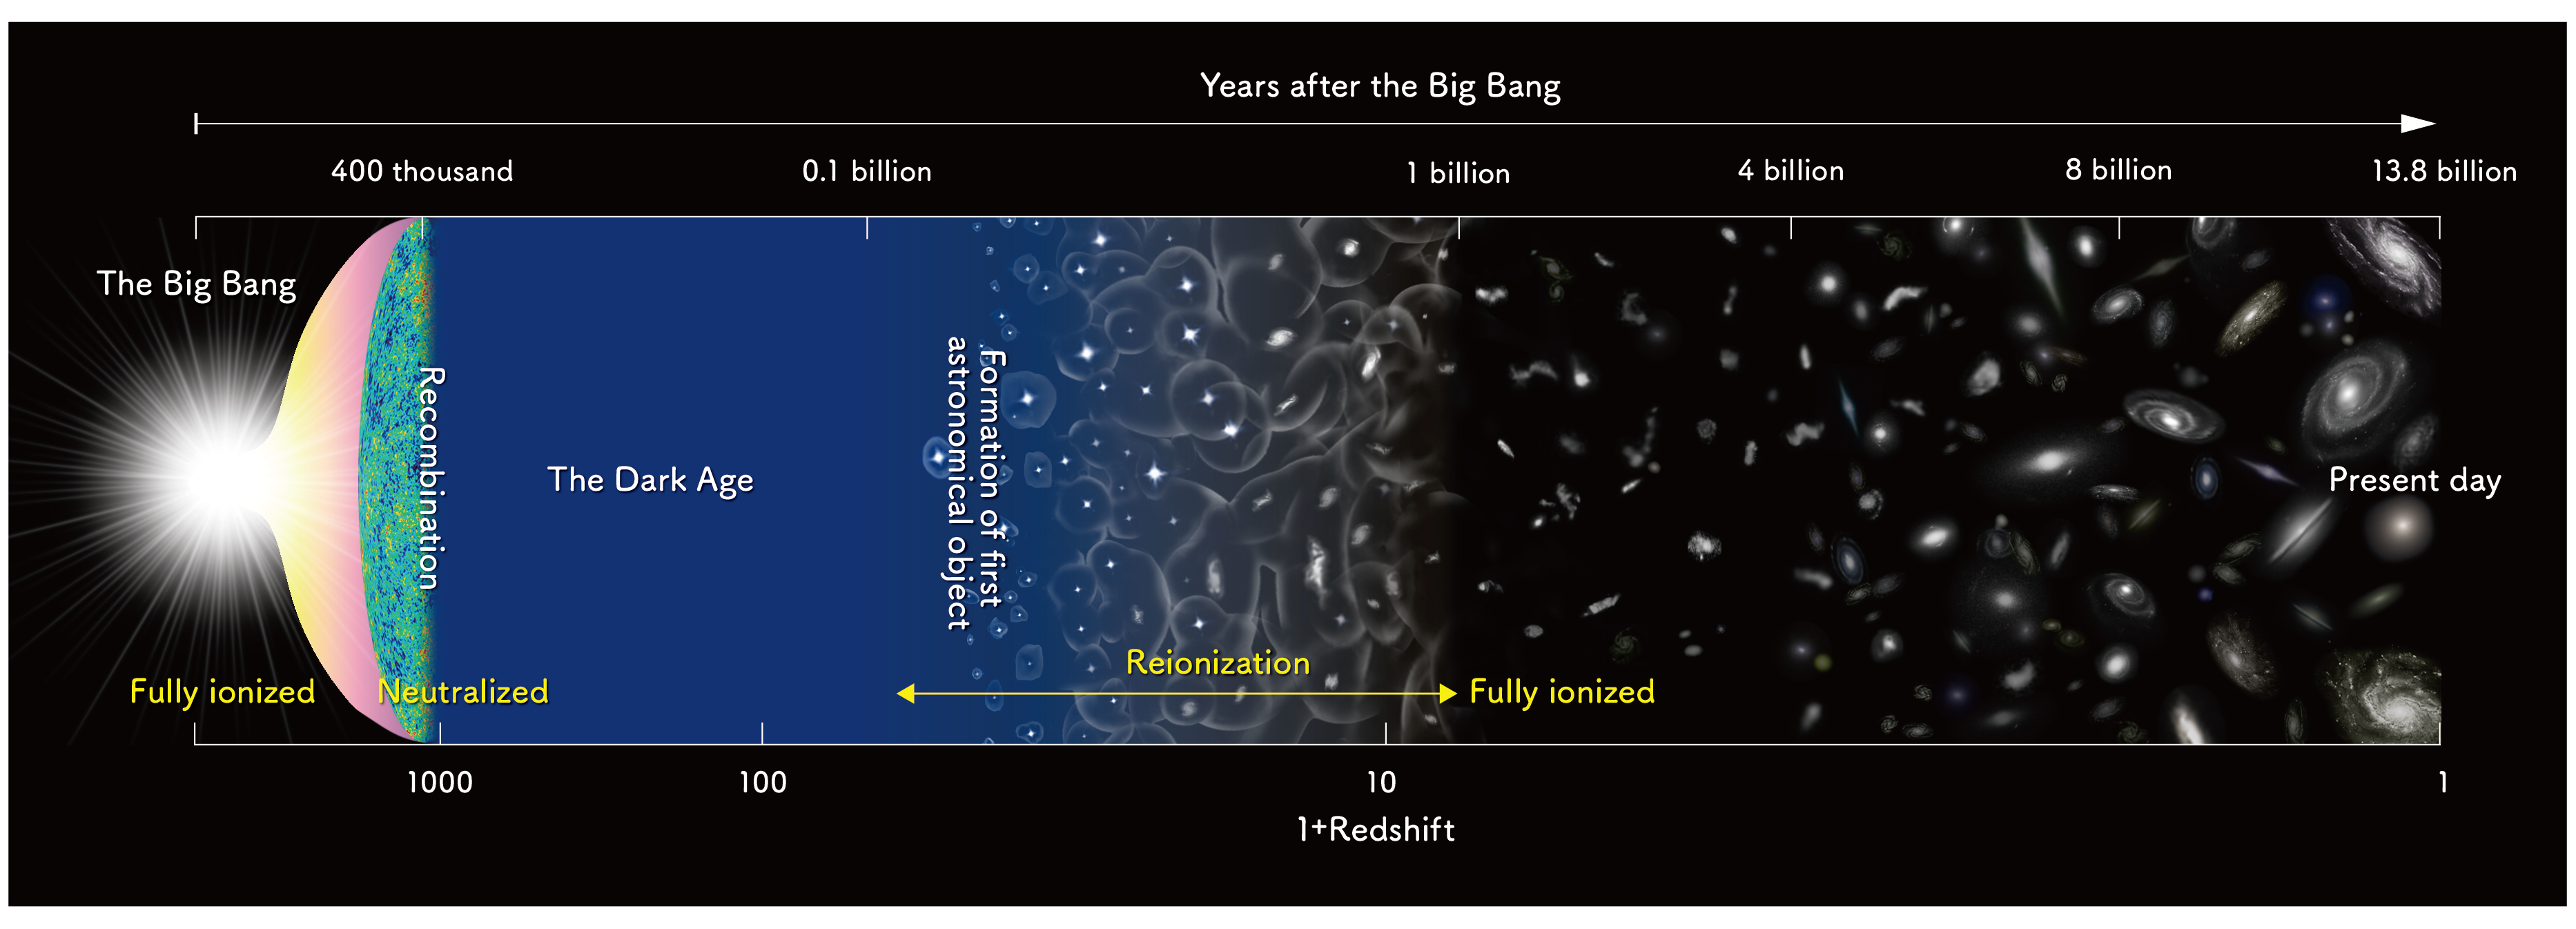
\includegraphics[width=\linewidth]{Figures/Reionizationtimeline.jpg}
		\caption{The cosmic history of the Universe from the Big Bang to its early years, through the dark ages to the epoch of reionization and the post-reionization epoch. Image credit:National Optical Astronomy Observatory}
		\label{Fig:timeline}
	\end{center}
\end{figure} 

Recombination occurred when the universe cooled enough for neutral hydrogen (HI) to form, around a redshift of $z$ $\sim1100$. Redshift enables us to gain access to the early age of the universe, which means that the higher the redshift, the further away we can look back in time. The redshift-wavelength relation is given by
\begin{equation}
\begin{split}
1+z & = \frac{\lambda_{obs}}{\lambda_{emit}}= \frac{1}{a}
\end{split}
\end{equation}
where $z$ is the redshift, $\lambda_{obs}$ is the wavelength of the observed signal, $\lambda_{emit}$ is the wavelength of the signal emitted, and $a$ is the Universe expansion scale factor. Before recombination, electrons were not bound to protons, and the universe contained ionized plasma known as photon-baryon fluid. Decoupled photons then formed the CMB~\citep{1965ApJ...142..419P}.

Subsequently, HI became the dominant baryonic component of the intergalactic medium (IGM) during the dark ages ($1100 \gtrsim z \gtrsim 30$). No measurements of the dark ages exist, and if hydrogen can be mapped in this era, valuable cosmological data can be produced~\citep{11, 2004PhRvL..92u1301L}.

There were density fluctuations in the distribution of matter, and the overdense regions collapsed under the influence of gravity, ultimately creating the first stars\st{. Thus, nuclear reaction resulted} \attention{and resulting} in Cosmic Dawn ($30\gtrsim z \gtrsim 10$). Energy from the first stars ultimately fully reionized the universe. Galaxies, galaxy clusters, and large-scale structures that exist in the present universe evolved after the first stars were born~\citep{2017arXiv170808521D, 2012AdSpR..49..433B}. 

Throughout the cosmological epochs, what is known is minimal because it is challenging to observe them directly. The growth of \SI{21}{cm} cosmology can fill the gaps in our knowledge of the universe's history~\citep{2012RPPh...75h6901P}. A brief overview of the universe's history has been given, and the next section will cover 21 cm cosmology corresponding to the dark ages and cosmic dawn in more detail.

\section{Cosmology with Redshifted 21-cm Emission}

Because hydrogen gas is the most abundant element in the universe, there is a concerted effort in the experimental community to develop telescopes for mapping neutral hydrogen via \SI{21}{cm} emission. This hydrogen line is an essential mechanism for probing the dark ages to the epoch of reionization (EoR)~\citep{2013PhRvD..87d3002L,2014ApJ...782...66P}. The generation of the hydrogen line (\SI{21}{cm} line or HI line) is due to the intrinsic electron and proton spins within the hydrogen atoms~\citep{book:832129}. The electron and proton spins can be oriented in either the opposing or the same direction, respective to each other. When the spins are opposing or antiparallel, the hydrogen atom is in the lower energy state. When the spins are parallel, the hydrogen atom is in a higher energy state. When an electron transitions from the higher energy state to the lower, \st{a photon is emitted only when the transition is from the higher to the lower state,} the hydrogen atom discharges a photon with a \SI{21}{cm} wavelength, equivalent to \SI{1420}{MHz}. The hyperfine splitting of the two energy states is equivalent to \(\Delta E =  5.9 \times 10^{-6} \ eV\). \autoref{Fig:21cm} shows the spin-flip transition process~\citep{16, book:832129}.

\begin{figure}
	\begin{center}
		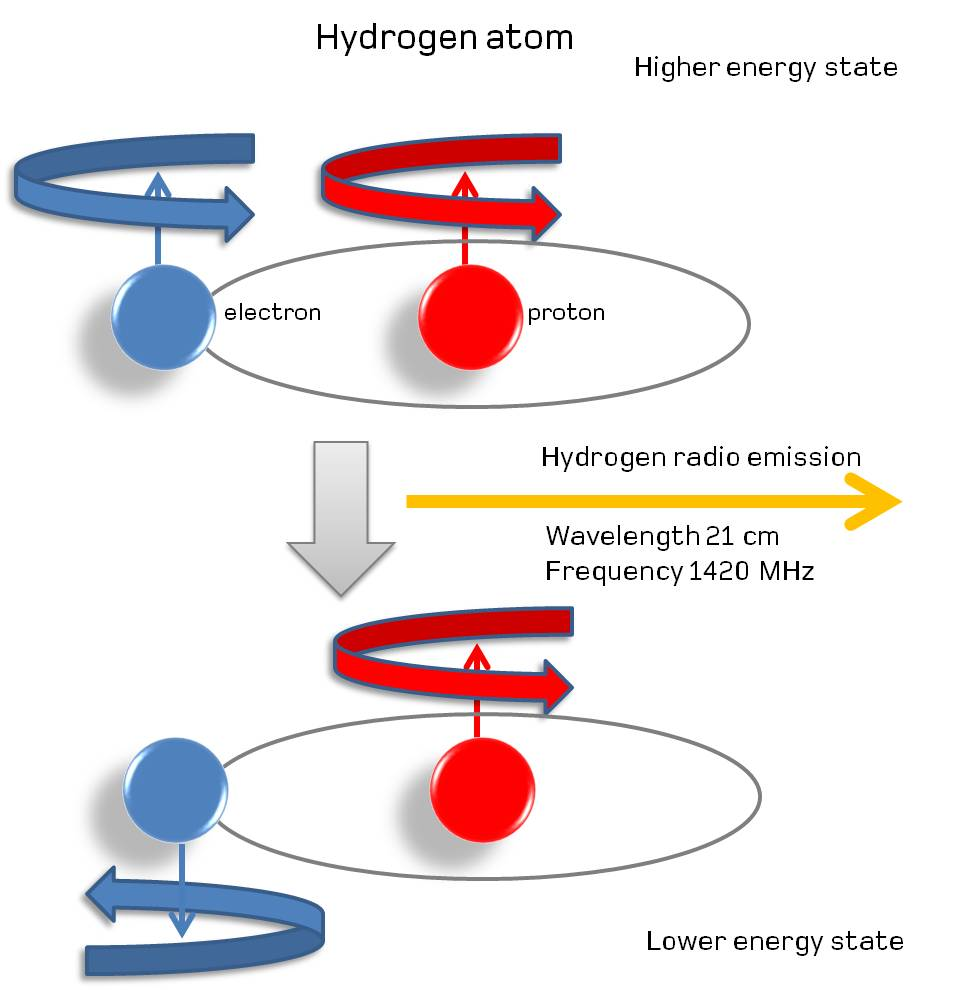
\includegraphics[width=0.5\linewidth]{Figures/Hydrogenemission1.jpeg}
		\caption{The formation of the \SI{21}{cm} wavelength line by the process of the spin flip transition where the hydrogen atom moves from one energy state to another. Image credit: {Square Kilometre Array}.}
		\label{Fig:21cm}
	\end{center}
\end{figure}

The populations of the low- and high-energy spin states, $n_0$ and $n_1$, define the spin temperature $T_s$:
\begin{equation}
\frac{n_0}{n_1} = \frac{g_1}{g_0}e^{(-E_10)/{k_B}{T_s}} = 3e^{{-T_*}{T_s}}.
\end{equation}
Here $\frac{g_1}{g_0}$ = 3 is the spin degeneracy of the triplet and singlet levels, and $T_{*}$ $\equiv$ $hc/k$ $\lambda_{21cm}$ = 0.068 K is the equivalent temperature of the hyperfine splitting of the two energy levels~\citep{2012RPPh...75h6901P}.

The \attention{globally averaged} brightness temperature $\delta$$T_b$ depends directly on $x_{HI}$, $z$, $T_S$, and $T_{CMB}$, but $T_S$ is heavily influenced by $T_K$ and the various coupling mechanisms. $x_{HI}$ is the fraction of neutral hydrogen \attention{[you define the neutral fraction in 2 places, and some of this text is redundant with the equation explanation below---condense where appropriate]}, the hydrogen spin temperature ($T_S$) is the excitation temperature of the 21 cm line, kinetic gas temperature, $T_K$, characterizes the thermal motion of atoms in the gas~\citep{2015aska.confE...1K,2006PhR...433..181F}. The equation	
\begin{equation}
\delta{T_b}\propto {x_{HI}}(1+z)^{1/2}({T_s}-{T_{CMB}})/{T_s}
\end{equation}
relates $\delta$$T_b$ to important factors which are \(x_{HI}\), the fraction of neutral hydrogen, redshift ($z$) and two temperatures, the spin temperature ($T_s$) and the CMB temperature ($T_{CMB}$).

Figure~\ref{Fig:epochs} describes the physical processes that are responsible for the frequency structures we see in the evolution of the sky-averaged 21 cm brightness temperature.

\begin{figure}
	\begin{center}
		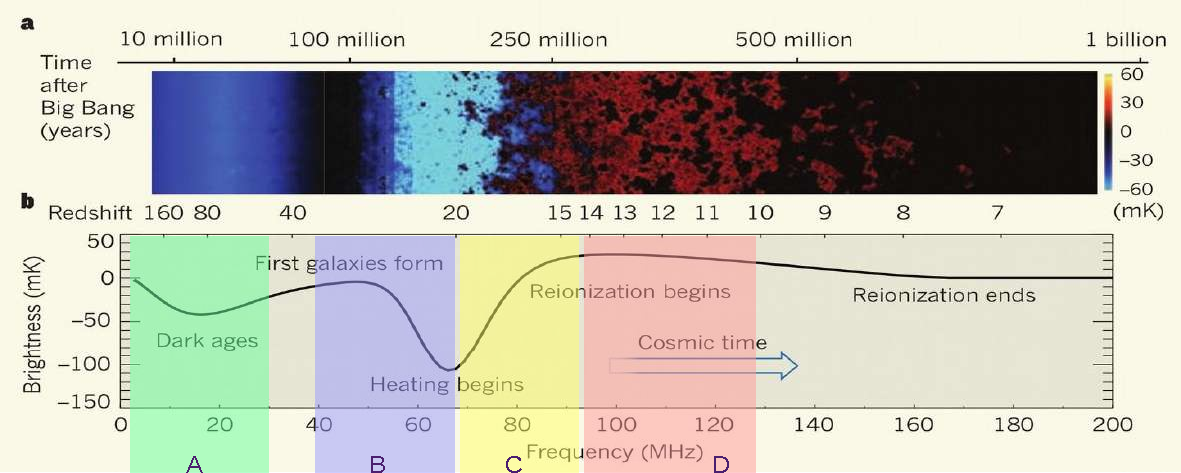
\includegraphics[width=\linewidth]{Figures/epo.pdf}\\
		\caption{Frequency structure of the globally averaged 21 cm signal: (a) shows the spatial and temporal evolution of the 21 cm brightness temperature and (b) shows the predicted time evolution of the globally averaged 21 cm brightness temperature ~\citep{2012RPPh...75h6901P}. There are different physical processes that govern the four highlighted (A to D) periods and the details are discussed in the main text.}			
		\label{Fig:epochs}
	\end{center}
\end{figure}

\subsection{Dark Ages}

The cosmic dark ages lie between recombination and cosmic dawn, beginning $\sim380,000$ years after the big bang and ending a few tens of million years later ($1100 > z > 30$),~\citep{2014arXiv1412.2096J} during which there were no luminous sources. The cosmic dark ages possess distinctive features that have never been explored to date. 

\textbf{Region A} in Figure~\ref{Fig:epochs} (green) highlights the dark ages period where the free electrons were no longer present. During this epoch, right after recombination, $T_K$=$T_\gamma$=$T_S$ where $T_\gamma$ is the temperature of the radiation background, typically set by the CMB so that $T_\gamma$ = $T_{CMB}$. During this period, matter that had separated from the CMB was cooled adiabatically as the universe expanded, which led to $T_K$ decreasing below $T_\gamma$~\citep{2006PhR...433..181F}. $T_S$ is initially coupled to $T_K$ as the collision between hydrogen atoms is effective at early times, resulting in $\delta T_b$ decreasing. As the universe expands and collisional coupling becomes ineffective, $T_S$ reverts to $T_\gamma$ because of CMB absorption, and $\delta T_b$ therefore eventually increases.

At this juncture, the most dominating matter in the universe was the dark matter and meager amounts of ordinary matter (neutral hydrogen and helium). After a few hundred million years, the dark and ordinary matter collapse together into halo-like structures through gravitational collapse, steadily cumulating physical matter and finally forming the first stars and galaxies, and that was the end of the cosmic dark ages~\citep{2003Sci...300.1904M}.

\subsection{Cosmic Dawn}

After the first stars' formation, their UV radiation couples to the HI line through the Wouthuysen-Field effect~\citep{2012RPPh...75h6901P}. Emission of Lyman Alpha photons by the first stars strongly couples $T_K$ and $T_S$ of the IGM; the described period is shown in \textbf{Region B} highlighted in purple. The coupling of $T_S$ to $T_K$ leads to a drastic absorption feature in $\delta T_b$. The absorption feature can be used to probe the formation processes of the first stars, with the potential of differentiating between Pop II and Pop III stars. \textbf{Region C} highlighted in yellow shows a period where the X-rays are emitted by hot accretion disks around the first stellar remnants (e.g., black holes) that effectively heat the cold HI gas. The heating of the neutral gas and constant coupling between $T_S$ and $T_K$ raised the overall spin-temperature to higher than the CMB temperature. Consequently, the 21-cm line became visible in emission at $z\sim15$. During radiation and heating, these first sources (possibly including mini-quasars) also ionized the gas around them, and a period of reionization started that is thought to have lasted until $z\sim5~to\sim 6$~\citep{2015aska.confE...1K}). The detailed $\delta T_b$ features are sensitive to the black hole properties and the progenitor's metallicity, offering further insight into first-star formation.~\citep{11}. \textbf{Region D} highlighted in red describes that when reionization begins, the neutral hydrogen supply is depleted ($x_{HI}$ decreases to zero), so $\delta T_b$ eventually also flatlines to zero because there is no more 21 cm signal left. 

\section{Hydrogen Line Observational Challenges}

Redshifted 21-cm radiation can penetrate dust and the Earth's atmosphere and is, therefore, an ideal tool for probing the history of the universe at any epoch of interest. However, ground-based telescopes and experiments are faced with several challenges when it comes to using the redshifted \SI{21}{cm} line emission to observe the dark ages, cosmic dawn, and the epoch of reionization. The primary challenges are human-made radio frequency interference (RFI), astrophysical foregrounds, ionospheric interference \attention{(the ionosphere is nearly opaque below 10~MHz)}, and instrumental systematics\st{, which is non-transparent below 10 MHz}. 

\subsection*{Brightness of Foreground Emission}

Foreground emission arises from both \attention{diffuse} Galactic \attention{structure} and extragalactic sources. The foreground emission's brightness temperatures are 4-5 orders of magnitude brighter than the cosmological \SI{21}{cm} signal. Galactic synchrotron emission is the primary foreground at low frequency and originates from the Galactic magnetic field's cosmic ray electrons' movement. Free electrons scattering off ions without being captured produces the Galactic free-free emission. The extragalactic foregrounds are predominantly radio-loud galaxies and quasars~\citep{2018RAA....18..114H, 2008MNRAS.389.1319J}.

\subsection*{Instrumental Systematics}\label{s:chall}

Global signal experiments measure total power and are therefore dominated entirely by systematics. \st{The faintness of the 21 cm signal presents a challenge as its characteristic scale is 0.1 mK. Few dipoles can be used to reach sensitivity.} \attention{[The point here is that 0.1 mK is actually ``easy'' to detect because it's ``bright.''  Replace the preceding text with the following sentence.]  The 21-cm absorption feature from cosmic dawn has a predicted amplitude of $\sim$0.1~mK.} To \st{include the order-of-magnitude} estimate \st{for} the amount of integration time needed to detect the cosmic dawn feature assuming statistical noise alone, \attention{we use the} \st{a} radiometer equation \st{is used, as follows},
\begin{equation}
T_{rms} = \frac{T_{sky}}{\sqrt{B. t_{obs}}},
\end{equation}
where $T_{rms}$ is the root mean square (rms) fluctuation of the sky temperature, $T_{sky}$ is the sky temperature, $B$ is the observation bandwidth, which can be varied, and $t_{obs}$ is the integration time in seconds. 
The required observing time can be estimated by
\begin{equation}
t_{obs} = \left ({\frac{T_{sky}}{T_{rms}}} \right )^2 \times \frac{1}{B}.
\end{equation}
For instance, $t_{obs}$ can be estimated to be \SI{3}{\hour} to reach the sensitivity of \SI{100}{\milli \kelvin} if $T_{rms} \sim 10 mK$, $T_{sky} \sim 1000 K$ and $B=$\SI{1}{\mega \hertz}. \st{Since the bandwidth can be varied, an integration time estimate of 1 day can be achieved. Though, the faintness of the 21 cm signal is a challenge, it can be alleviated with prolonged observations coupled with a large number of dipoles and/or a large effective area.} \attention{This calculation shows that statistical noise is typically not a limiting factor for cosmic dawn experiments.}

\subsection*{RFI}

Besides astrophysical challenges, human-made RFI saturates \st{the} \attention{manyfg
} frequency bands, increasing the need for isolated remote deployment sites. RFI can be orders of magnitude brighter than Galactic and extragalactic foregrounds. Unfortunately, RFI introduces a reduction in sensitivity in two separate but distinct ways: direct contamination by having similar spectral characteristics and overpowering the \SI{21}{\centi \meter} signal. The cosmic dawn signal \st{correlates} \attention{coincides} with the FM band (\SIrange{88}{108}{\mega \hertz} corresponding to 15$>$z$>$12), and FM contamination is especially predominant. Like radio transmitters that are run on the ground, satellite or aircraft communications often contribute to RFI. These RFI origins need not be nearby in many instances. Ionized meteor tracks, for example, are known to reflect RFI from remote areas. Inadequately shielded electronics can create self-generated RFI in the telescopes. RFI overpowers the signal from sources of astrophysical origin; therefore, mitigation must be applied. The foremost fundamental procedure for RFI mitigation is to prevent RFI in telescopes by deploying in remote areas. Other than site selection, there needs to be RFI removal during data analysis~\citep{2020PASP..132f2001L}. 

As much as RFI is challenging to avoid, there are a few restricted circumstances where it can be useful. The Orbcomm satellite transmission around \SIrange{137}{138}{\mega \hertz}, for instance, serves as a calibrator source that can be used to provide analytical mappings of an antenna's main beam patterns. With such satellites in low-Earth orbits that precede over time, these sources travel through the field of view of an antenna rapidly and regularly,  allowing a relatively densely sampled mapping of the primary beam~\citep{2015RaSc...50..614N, 2018PASA...35...45L}. 

\subsection*{Ionospheric Contamination}

The Earth's ionosphere also introduces significant fluctuations, which becomes increasingly refractive and turbulent below 100 MHz and becomes practically opaque below 10 MHz. In order to minimize RFI and ionospheric contamination, there have been proposals to observe long wavelengths from space-based telescopes further away from the ionosphere of our planet. These space-based telescopes do not exist yet, and there are several ground-based experimental efforts to understand how well we can make measurements from Earth~\citep{2019arXiv190710853C, 2019arXiv190804296K}. At night near-polar latitudes have lower plasma cutoff frequencies, and the cutoff is reduced during solar minima.

\section{Previous Cosmic Dawn and Low-frequency Experiments}

The \SI{21}{cm} wavelength of hydrogen gas is being observed by several experiments that are \st{modeled} \attention{designed} for Hydrogen mapping in our universe. Despite the challenges that are encountered in 21 cm cosmology, many experiments are nevertheless underway. This section highlights experiments aimed at frequencies corresponding to the dark ages ($1100 \lesssim z \lesssim 30$) and cosmic dawn ($30 \lesssim z \lesssim 10$).

\subsection{Global Signal Experiments for Cosmic Dawn}

The global signal experiments are most commonly located in remote RFI-quiet areas using single antennas with a large solid angle observing total power. However, there have been suggested and attempted innovative methods using interferometry. 

The Experiment to Detect the Global EoR Signature (EDGES) is located at Murchison Radio-astronomy Observatory (MRO) in Western Australia. The project's goal is radio detection of characteristic hydrogen signatures from cosmic dawn and the epoch of reionization. EDGES consists of a high-band instrument operating over the 90-200 MHz (14 $>$ z $>$ 6) range, a mid-band instrument operating over 60–160 MHz, and a low-band instrument that is sensitive to the 50-100 MHz (27 $>$ z $>$ 13) range~\citep{2017ApJ...835...49M}. 

The first detection of the 21 cm global signal was reported by \citet{2018Natur.555...67B} as a flattened absorption profile centered at a 78.1 MHz frequency, with an amplitude of 0.53 K and width of 18.7 MHz. \st{It} \attention{The amplitude} is more than a factor of two \attention{larger} \st{brighter} than the most optimistic model where no heating occurs until $z \sim$ 17, thus suggesting a hotter background or a colder than expected primordial gas.  \st{In terms of collisional dark matter}~\citet{2018Natur.555...71B, PhysRevD.98.103005} \st{and independent verification by similar experiments, the detection has called for an interpretation of newer physics.} \attention{The detection has spurred multiple interpretations of new physics, including collisional dark matter~\citep{2018Natur.555...71B, PhysRevD.98.103005}.  Independent verification by similar experiments is therefore of utmost importance.}

\st{EDGES experiment has been discussed, and the o}\attention{O}ther global signal experiments are summarised in Table~\ref{Tab:CD}. The included experiments are the Cosmic Twilight Polarimeter (CTP,~\citet{2019ApJ...883..126N}),  Large aperture Experiment to Detect the Dark Ages (LEDA,~\citet{2012JAI.....150004T, 2018MNRAS.478.4193P}), Mapper of the IGM Spin Temperature (MIST,~\citet{inproceedings}),   \prizm,~\citet{2019JAI.....850004P}, Radio Experiment for the Analysis of Cosmic Hydrogen (REACH,~\citet{8879199}), and the Shaped Antenna measurement of background RAdio Spectrum 2 (SARAS2,~\citet{2013ExA....36..319P})  

\begin{table}
	\centering
	\begin{tabular}{ c|ccc} 
		& Site & Frequency & Instrumental Approach \\
		\hline
		CTP & Troy, Virginia & 60--120 MHz & Dual-polarization Dipole \\
		
		LEDA & Owens Valley & 10--88 MHz & 251 Dual-polarization Dipoles \\
		
		MIST & MARS & 5--200 MHz & One Dipole Antenna \\
		\prizm\ & Marion Island & 30--200 MHz & 2 Dual-polarization Dipoles \\
		REACH & South African Karoo desert & 50--200 MHz & Monopole Antenna \\
		SARAS2 & Gauribidanur Obs., India & 87.5--175 MHz & Fat-dipole Antenna \\
		\hline
	\end{tabular}
	\caption{Active and upcoming global signal experiments. CTP, LEDA, MIST, \prizm\, REACH and SARAS 2 experiments with their deployment sites, frequency ranges and instrumental approach.}
	\label{Tab:CD}
\end{table}  

\subsection{Imaging below 30 MHz}

{\bf{Long Wavelength Astronomy Background}}

The father of radio astronomy, Karl G. Jansky, played a massive role in the inauguration of radio astronomy dating back to 1931. At that time, he was an employee at the Bell Telephone Laboratories as a radio engineer. Jansky was allocated to study and solve the problem that hindered the radio communication systems. Using highly directive antenna arrays shown in \autoref{Fig:Jansky}, he discovered that the static caused the radio frequency noise that hindered the communication systems from thunderstorms~\citep{book:BasicsofRA, book:RA}.

\begin{figure}
	\begin{center}
		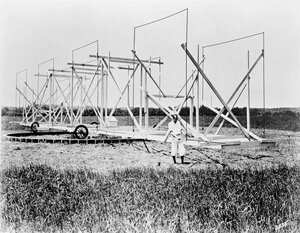
\includegraphics[width=0.7\linewidth]{Figures/jansky1.jpg}
		\caption{Jansky's highly directive antenna arrays which he used to discover the cause of RFI that hindered the communication systems at Bell Telephone Laboratories~\citep{book:BasicsofRA}}.
		\label{Fig:Jansky}
	\end{center}
\end{figure}

The antenna that he constructed operated at an approximated frequency of \SI{20}{MHz}, corresponding to an approximate long wavelength of \SI{15}{m}. He further found radio radiation from the Galactic Center at the operating frequency. Out of interest in Jansky's instigating discoveries, Grote Reber designed a radio telescope that operated at a range of approximately \SI{10}{MHz} to \SI{160}{MHz} (\SI{30}{m}-\SI{2}{m} wavelength) in 1937. He discovered that the \st{authoritative} \attention{dominant} source at longer wavelengths was the Milky Way. Furthermore, he realized that the radio telescope acts like a bolometer or a device to measure the heat. The antenna's radiation resistance measures an equivalent temperature of a distant part of space to which the 24 antenna response pattern projects it~\citep{1988JRASC..82...93R, CosmicStatic,2012PASP..124.1090H}.

Because of the research done for the communication systems, radio astronomy was born and expanded to radio astronomy and astrophysics~\citep{2012PASP..124.1090H}. The hydrogen line research area had an accelerated discovery, which was allocated an operating frequency of \SI{1420}{MHz} (\SI{21}{cm} wavelength) ~\citep{10.2307/530765}. After all these discoveries, the long-wavelength astronomy fascination has been resuscitated in the present epoch.

{\bf{Long Wavelength Astronomy Experiments}}

There are quite a few low-frequency experiments, but this document will briefly discuss a few measurements that exist at $\lessapprox$ 30 MHz. Two of these experiments represent the lowest frequencies measured to date (Reber's antenna, RAE-B). The other two represent the highest resolutions achieved in this frequency range (DRAO, OVRO-LWA).

Grote Reber constructed a state-of-the-art telescope operating at very low frequencies between 0.52 MHz and 2.1 MHz, which had 192 dipoles. At 2.1 MHz, the array had a resolution $\sim$ 5 \degree and was able to map the sky. The measurements were dominated by Galactic emission and the ionosphere as shown in Figure~\ref{Fig:Rebermap}~\citep{1988JRASC..82...93R}. 

\begin{figure}
	\centering
	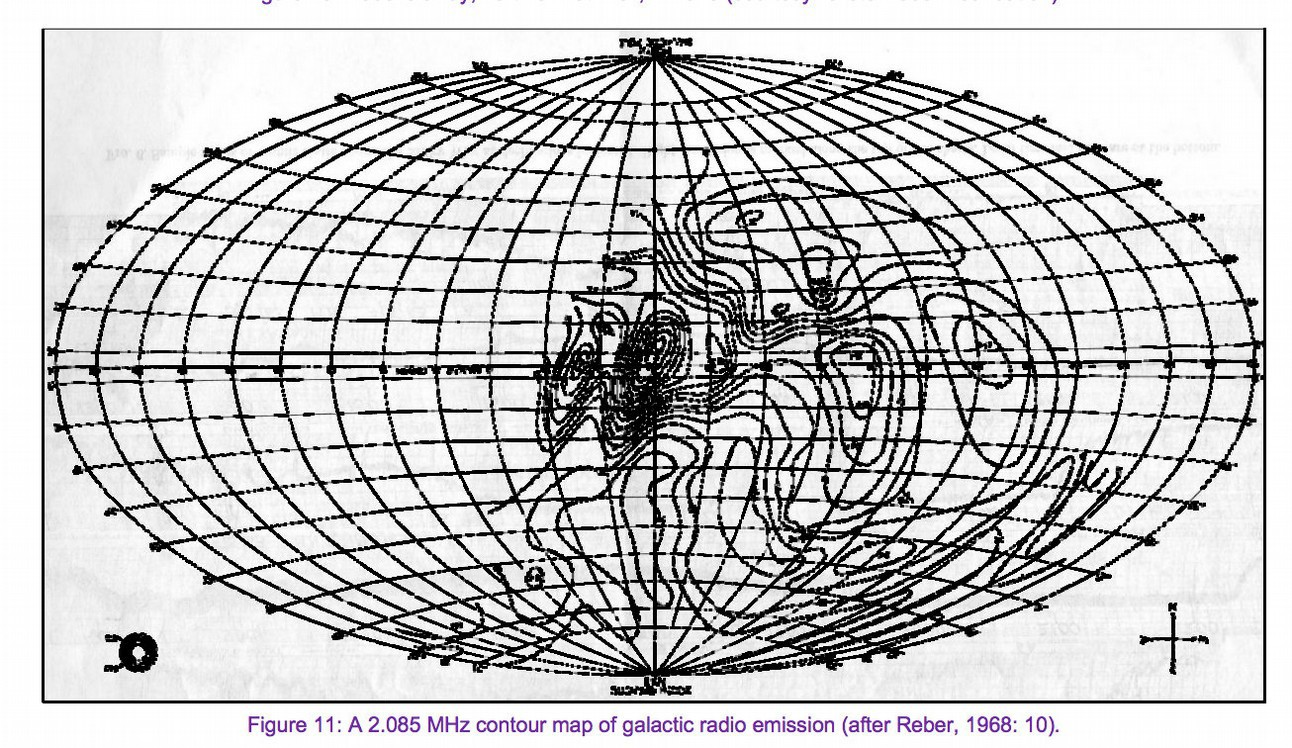
\includegraphics[width=0.7\linewidth]{Figures/Rebermap}
	\caption{Grote Reber's state-of-the-art map. The constructed array operated at very low frequencies between 0.52 MHz and 2.1 MHz and at 2.1 MHz, the array had a resolution of $\sim$ 5 \degree. It was able to map the sky, and the measurements were dominated by Galactic emission and the ionosphere~\citep{1988JRASC..82...93R}.}
	\label{Fig:Rebermap}
\end{figure}

The Radio Astronomy Explorer-2 (RAE-2) operated between 25 kHz and 13 MHz, with the primary science goal of radio measurements of our Galaxy, the Sun, Earth, and all the other planets. The resolution of this experiment is $\sim$10 \degree at \SI{4.7}{\mega\hertz}~\citep{1975A&A....40..365A}. \st{Thus far, the data presented is the only data that exists, and nothing exists elsewhere.}

Higher-resolution experiments include the OVRO-LWA, Dominion Radio Astrophysical Observatory (DRAO) 22 MHz telescope, and the DRAO \SI{10}{\mega\hertz} array. The OVRO-LWA operates at frequency ranges of \SI{36.528}{\mega\hertz} and \SI{73.152}{\mega\hertz}. At these frequencies, it has an angular resolution of \SI{15}{\arcminute}~\citep{2018AJ....156...32E}. The DRAO telescope operated at 22 MHz, and its resolution ranges between $\sim$1.1 \degree - 1.7 \degree. Its primary science goal was to measure the emission from discrete sources and observe our Galaxy's emission from its environment~\citep{1999A&AS..137....7R}. The DRAO 10 MHz array operated had a resolution of $\sim$ 2  \degree, and it was first used for discrete sources and was later used to map the large-scale structure of the background radiation~\citep{1976MNRAS.177..601C}.

\section{Structure of this Thesis}


The following is the outline of this thesis: in Chapter 2, 
Marion Island is introduced, the observing location of \prizm\ and \albatros. A summary of my voyage to Marion will also be provided. Chapter 3 will provide a full description of the \albatros\ instrument. Chapter 4 will provide a brief description of the \prizm\ instrument and present a summary of various system stages. In Chapter 5, preliminary results will be presented and conclude in the same chapter. My main contributions are listed below:
\begin{itemize}
	\item Designing a prototype solar power supply system in preparation for the 2019 Marion voyage, 
	\item Site inspection and installation of the first \albatros\ autonomous station at Marion Island in 2019,
	\item Helping with the revision and new designs of the \prizm\ subsystems, including the front end electronics enclosure, switch control circuit, 
	\item Designing the \prizm\ second stage electronics enclosure, which was in preparation for the 2020 deployment that did not happen.
\end{itemize}

	\chapter{Observing at the Marion Island Site}

\attention{You have all the right factors for site selection in the
  paragraphs below, but I'll suggest reorganizing for clarity.  Start
  by explicitly stating that there are several factors that need to be
  considered when choosing a site for PRIZM/ALBATROS, and that those
  are RF quietness, ionospheric conditions, accessibility, and ability
  to support long baselines.}

Low-frequency observations require high angular resolution to improve the experiment's sensitivity. Systematics discussed in \S\ref{s:chall} widely dominate the experiments operating at frequencies $<$\SI{200}{MHz}. RFI from the frequency modulation (FM) transmitters is a substantial contributor in the low-frequency regime; thus, FM contamination is widespread into observation bands. Observing from remote deployment sites is a solution to the FM band contamination issue. Before site selection and deployment, radio environments must match the specific instrument's requirements when assessed. Accessibility is a common challenge that arises from remote site selection. Therefore, choosing a good observing location is generally a balance between	accessibility and radio-quietness. 

Marion Island was chosen as the observing site for Probing Radio Intensity at high-Z from Marion~\citep[\prizm;][]{2019JAI.....850004P} and the Array of Long Baseline Antennas for Taking Radio Observations from the Sub-Antarctic~\citep[\albatros;][]{2020arXiv200812208C} \attention{[since you've defined PRIZM and ALBATROS as acronyms already, there's no need to redefine them here]} after evaluating the mentioned factors. Marion Island is the exceptionally radio-quiet environment for low-frequency observations, although the site is only accessible annually. The next section discusses the location in more detail.

\section{Marion Island}

Marion Island is a research base that forms part of the Prince Edward Islands shown in Figure~\ref{fig:marion}, located in the southern Indian Ocean at \ang{46;54;45}S, \ang{37;44;37}E. The South African National Antarctic Programme (SANAP) and the South African Department of Environmental Affairs (DEA) operate the research base shown in Figure~\ref{fig:base}. \attention{[I edited some of the text in the next few sentences.]} The island is $\sim$ \SI{2000}{\kilo\metre} from the nearest continental landmasses, has an area of 290~km$^2$, and the main base is positioned on the northeast side. Marion Island has a volcanic origin, and the terrain is scattered with many secondary craters and small lakes. There is abundant snow and rain, and the vegetation is mainly mosses and ferns. The lowland regions are marshy due to high precipitation. It is extremely windy and	mostly cloudy throughout the year.

\begin{figure}
	\centering
	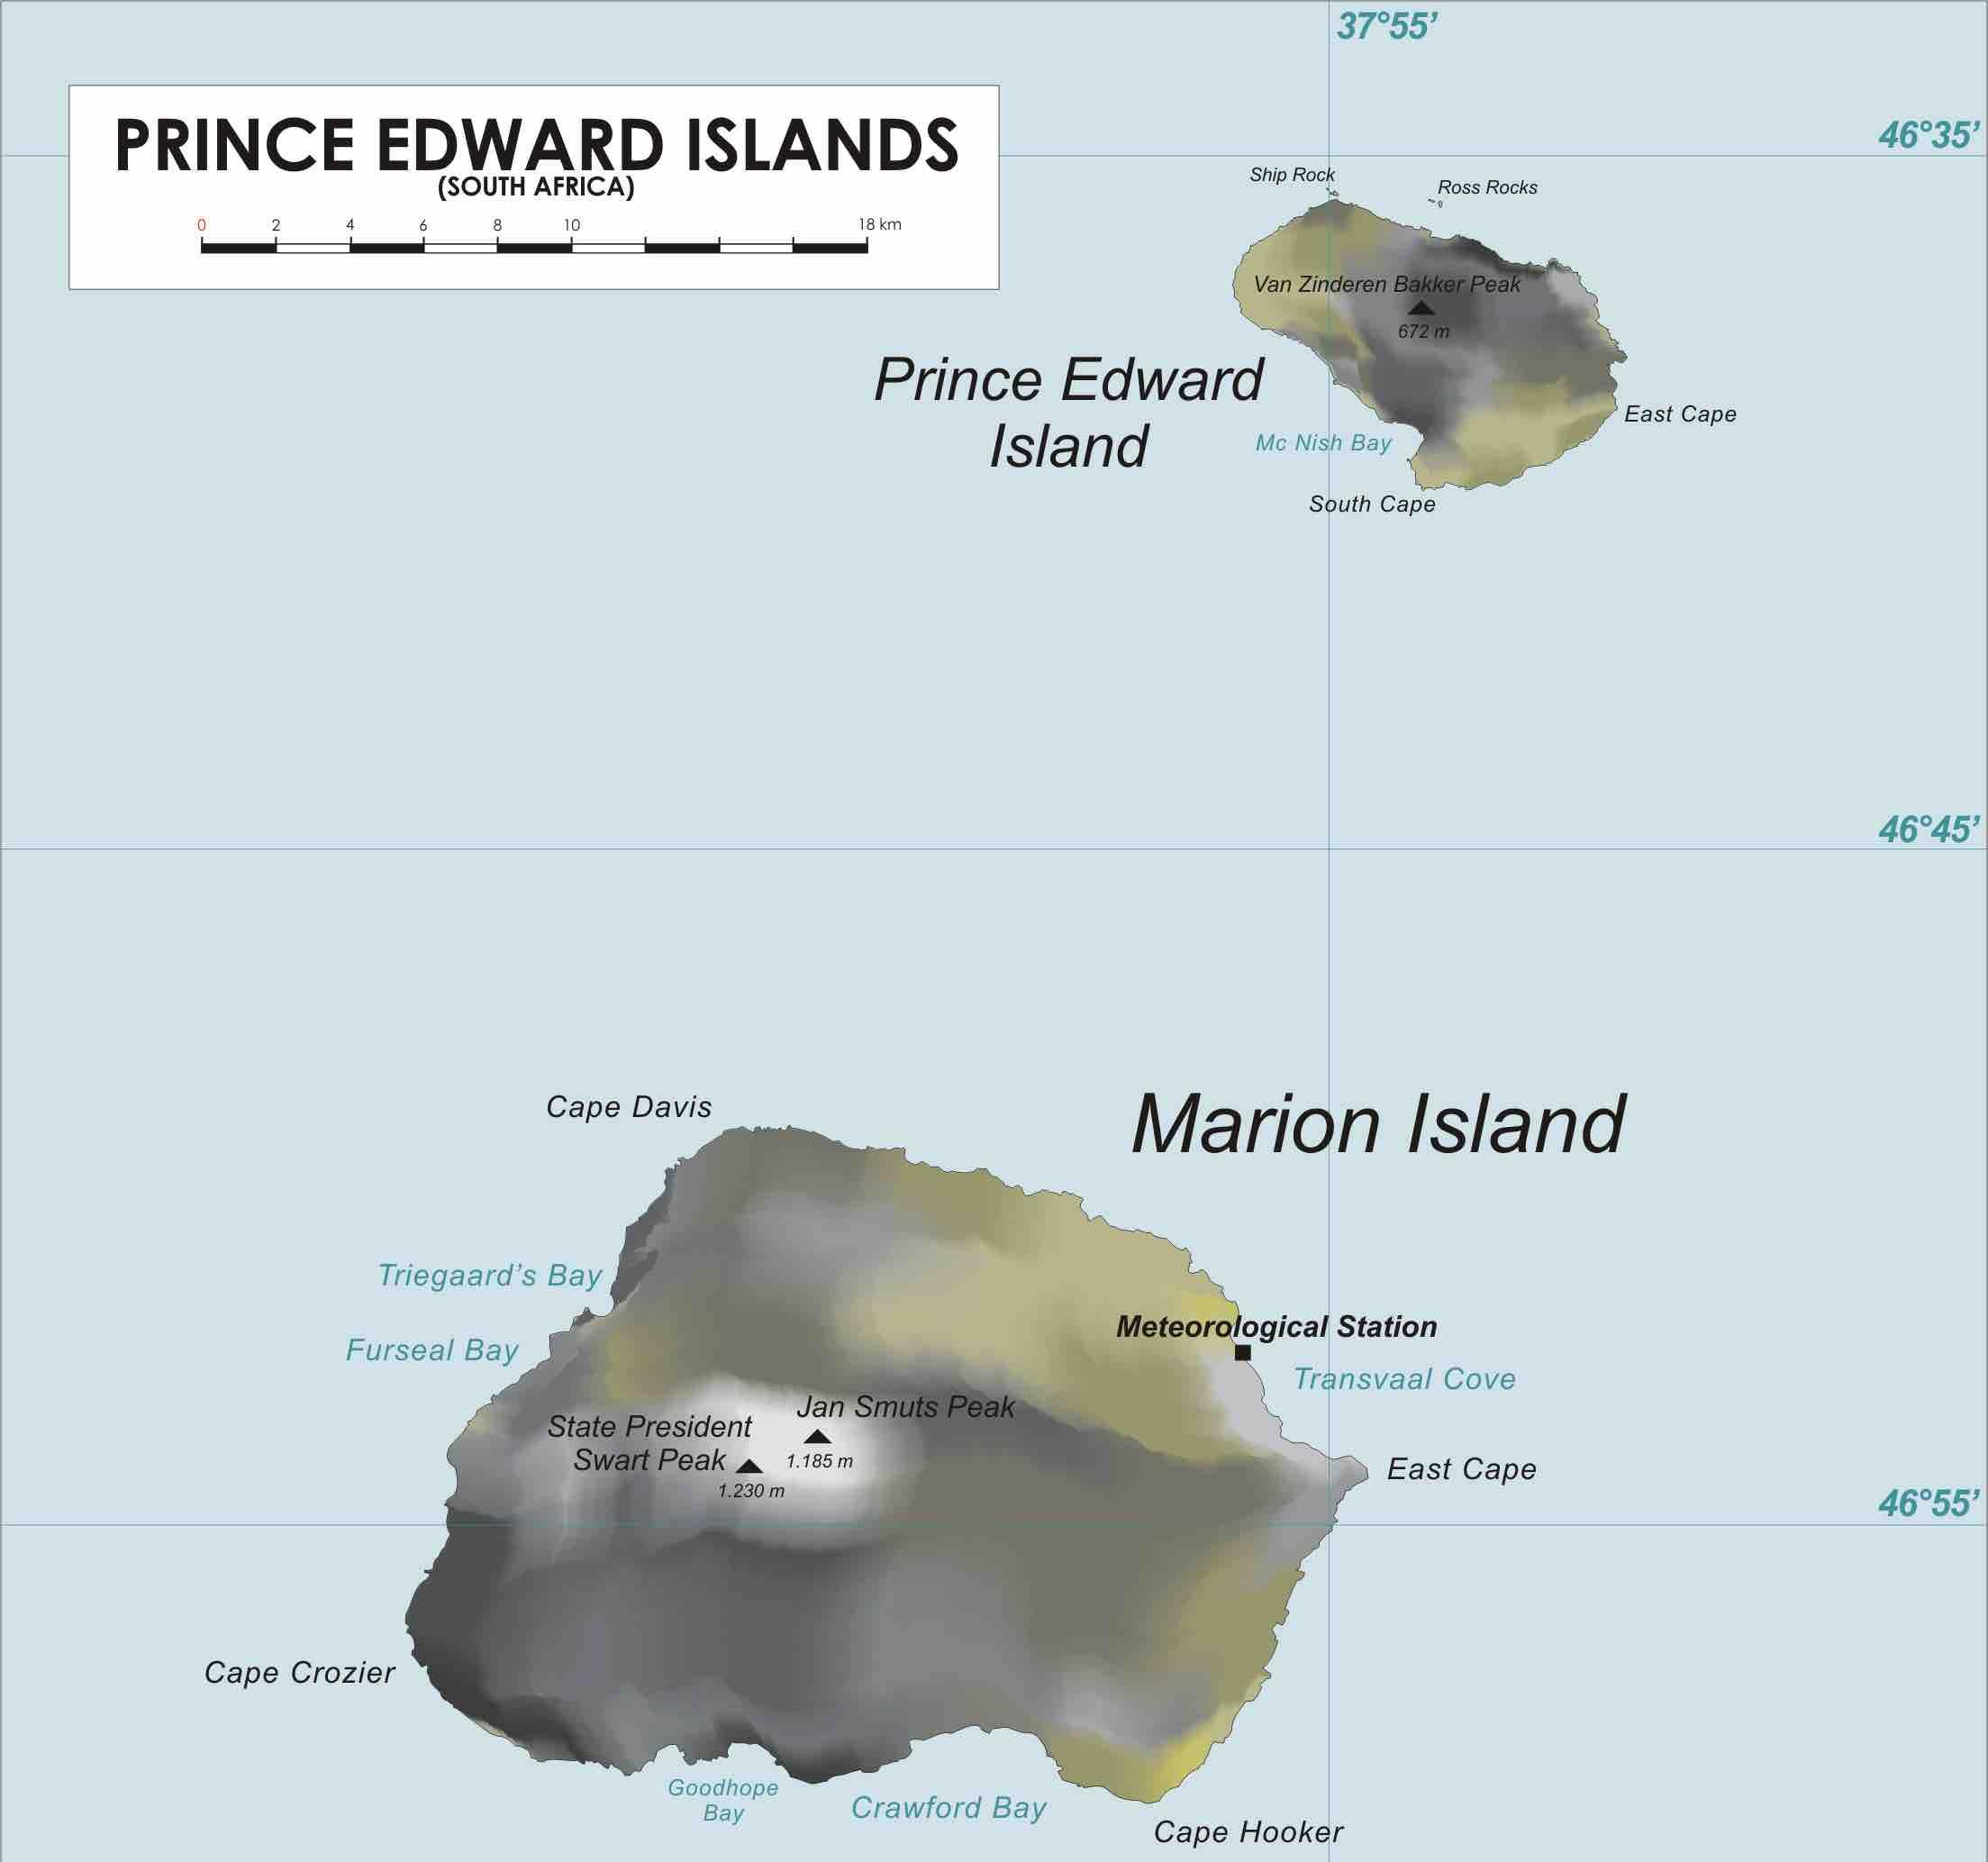
\includegraphics[width=\linewidth]{Figures/marion}
	\caption{The two islands in the Prince Edward Islands are Prince Edward Island and Marion Island, located in the sub-Antarctic Indian ocean. \attention{[I made some minor edits.  Include a source for the figure.]}}
	\label{fig:marion}
\end{figure}

\begin{figure}
	\centering
	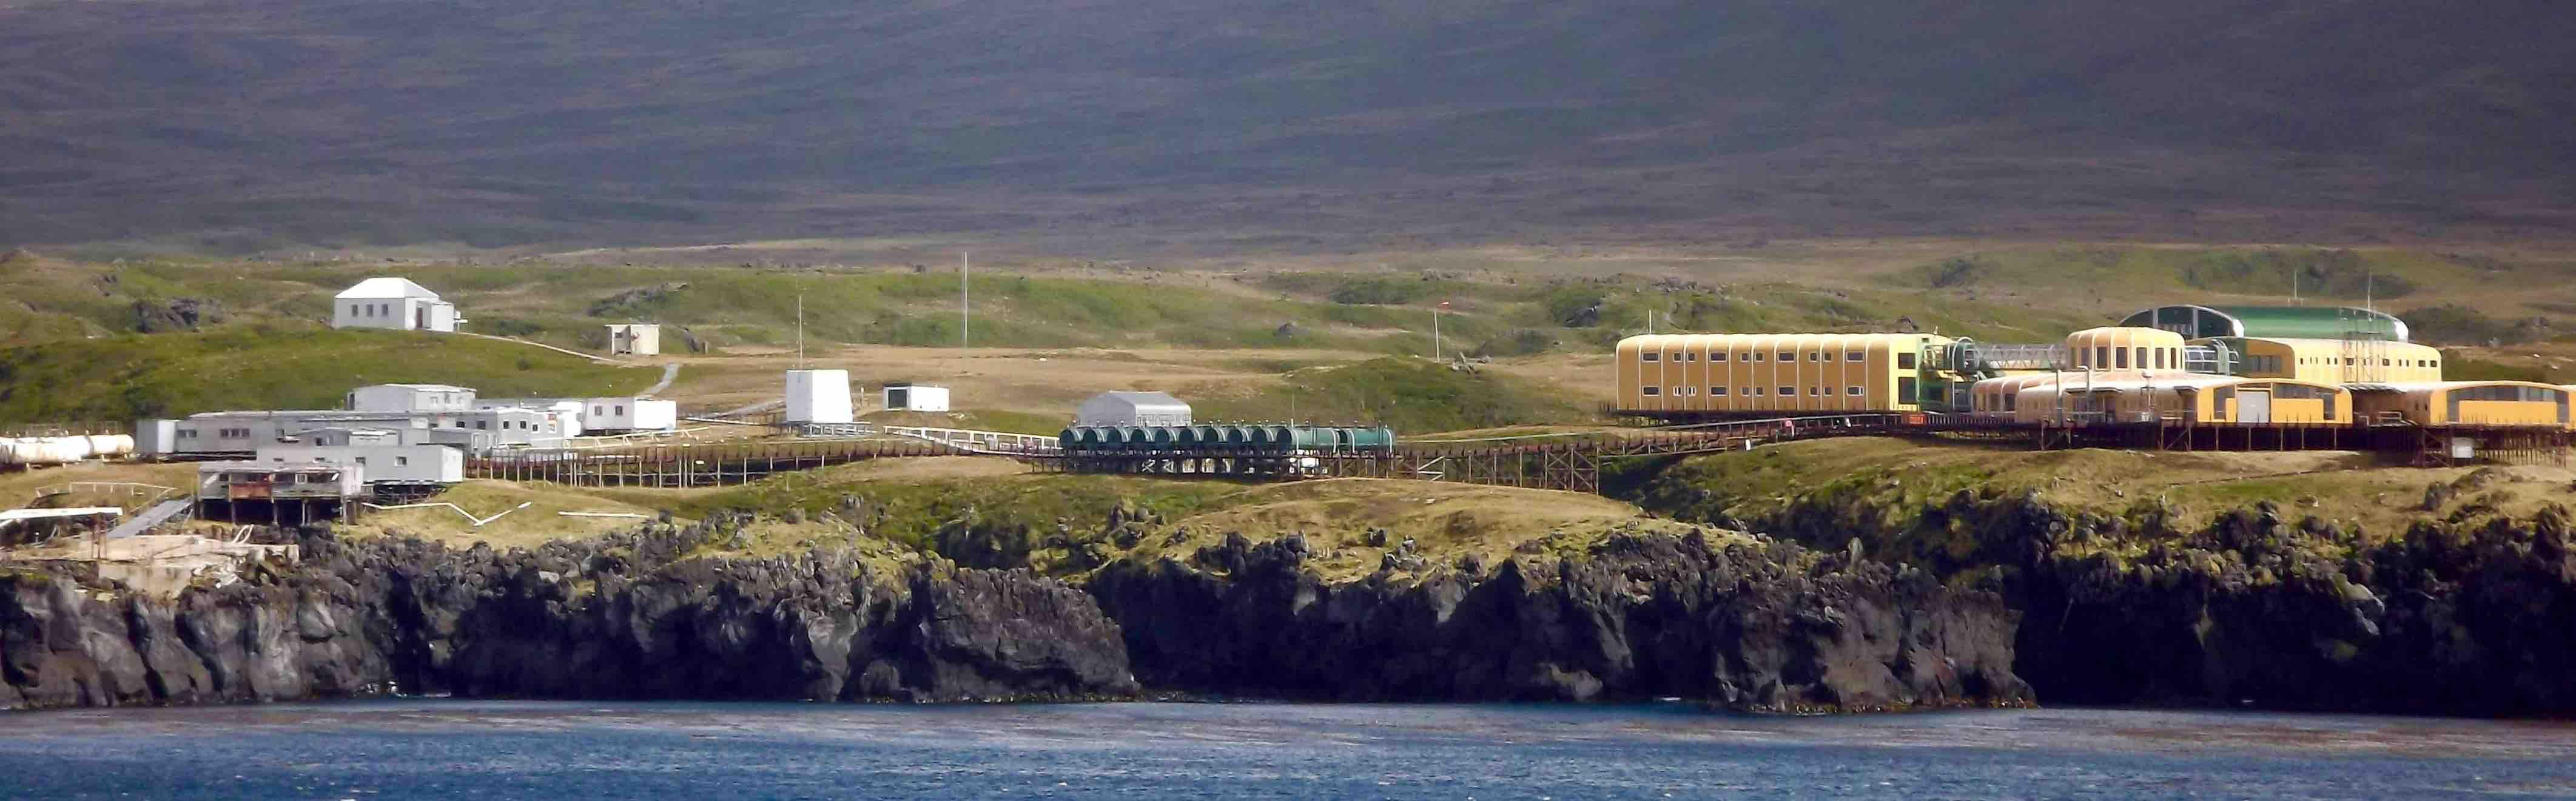
\includegraphics[width=\linewidth]{Figures/base}
	\caption{Marion Island new (yellow buildings) and old base (white buildings). The green building partially visible behind the new base is the emergency base that serves as a helipad and a hangar for helicopter operations.}
	\label{fig:base}
\end{figure}

The DEA owns the S. A. Agulhas II \footnote{\url{https://en.wikipedia.org/wiki/S. A. Agulhas II}}, a South African ice-breaking polar supply and research ship that services the island every year in April. During the relief voyage in April, three weeks are spent on the island deploying and maintaining \st{the existing} instruments. Marion Island \st{caters for various} \attention{has been traditionally used for the} research fields \attention{of space weather, geology,} \st{such as} meteorology, mammalogy, ornithology, and botany. The main Marion base accommodates all the researchers participating in the relief voyage and overwintering team members. Figure~\ref{fig:site} shows the nine rest huts (Kildalkey, Watertunnel, Cape Davis, Grey-headed, Mixed Pickle, Repettos, Rooks, Swartkops, and, Katedraal) that researchers use while traversing the island. The \prizm\ instrument was deployed at the \prizm\ site \attention{[``PRIZM site'' isn't very descriptive; replace this with e.g. 4km southwest of the main base]} (\ang{46;53;13}S, \ang{37;49;10.7}E) as the first radio astronomy experiment in Marion Island, followed by the \albatros\ \st{experiment} \attention{pathfinder instruments} on the same site. 

\begin{figure}
	\centering
	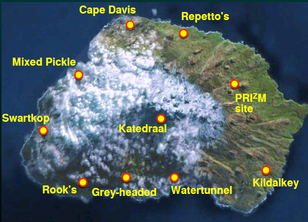
\includegraphics[width=\linewidth]{Figures/site}
	\caption{Marion Island rest huts and the \prizm\ site where the first radio astronomy instrument was deployed and subsequently \albatros\ pathfinder.}
	\label{fig:site}
\end{figure}

\section{Advantages of Observing from Marion Island}

\st{The discussion that follows is described by} \attention{This section presents a brief overview of the site selection process on Marion, and a full description is available in}~\citet{2019JAI.....850004P} \attention{[note the difference between citep, which places cites in parentheses, and citet, which includes cites as part of the text]}. In choosing the observing site for \prizm\ \attention{[don't forget to put the backslash at the end of prizm so that it doesn't gobble the following space; I've fixed here, but I'll leave it up to you to do a search and replace elsewhere]} and \albatros, several radio spectrum measurements were done on different sites, including the South African Karoo desert. The radio-quiet environment of Marion Island surpasses that of the South African Karoo desert, as shown in Figure~\ref{fig:karoo}. At Marion Island \st{site}, there is no evident detection of RFI contamination in the FM band\attention{, and the only significant RFI visible within the PRIZM operating range is} \st{besides the} Orbcomm satellite transmission \st{visible} at \SIrange{137}{138}{\mega\hertz} and the \SI{250}{\mega\hertz} FPGA clock artifact visible at \SI{125}{\mega\hertz}. The enhanced RFI from meteor scattering \attention{[expand and explain this a bit more: ionization trails scatter distant RFI sources]} is a common \st{threat} \attention{phenomenon} in several remote sites excluding Marion Island, as there have not been evident measurements of such RFI.

\begin{figure}
	\centering
	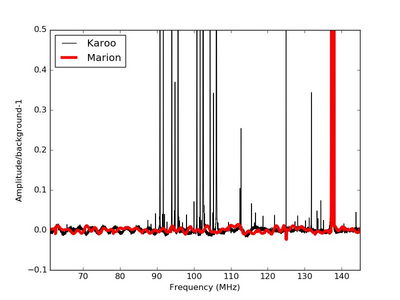
\includegraphics[width=\linewidth]{Figures/karoo}
	\caption{Comparison of radio spectrum on Marion (thick red) and in the Karoo desert (thin black). The fractional amplitude above a background fit to the raw and uncalibrated data without RFI excision. Orbcomm satellite transmission is visible at 137–138 MHz; there is no visible RFI in Marion's data. The feature at 125 MHz is an artifact of the 250 MHz FPGA clock and not due to RFI~\citep{2019JAI.....850004P}}
	\label{fig:karoo}
\end{figure}

Figure~\ref{fig:rfi} shows the RFI spectrum comparison between the \prizm deployment site \SI{4}{\kilo\metre} away from the island's main base. Locally generated RFI less impacts the \prizm site \attention{[rework this sentence to describe that we wanted a site for PRIZM that was far enough away from the main base to keep locally generated RFI at a minimum while still being a reasonable hiking distance]}. Junior's Kop situated between the deployment site and the island's main base provides enhanced RFI shielding of \SI{\sim60}{\decibel} \attention{[note that 60~dB is a combination of attenuation from the land mass in Junior's, plus the distance]}. The helicopter was operating near the base when the RFI measurements were taken and transmitting at a frequency of \SI{123.45}{\mega\hertz} \attention{[expand this sentence a bit more and explain that the helo transmission line was a fortuitous source of RFI that allowed us (roughly) calibrate the relative levels at Junior's vs the base]}.  \attention{Somewhere in here, you may also want to mention the constraint that we wanted a site with reasonably dry and even terrain, i.e. not in a mire. :-)}

\begin{figure}
	\centering
	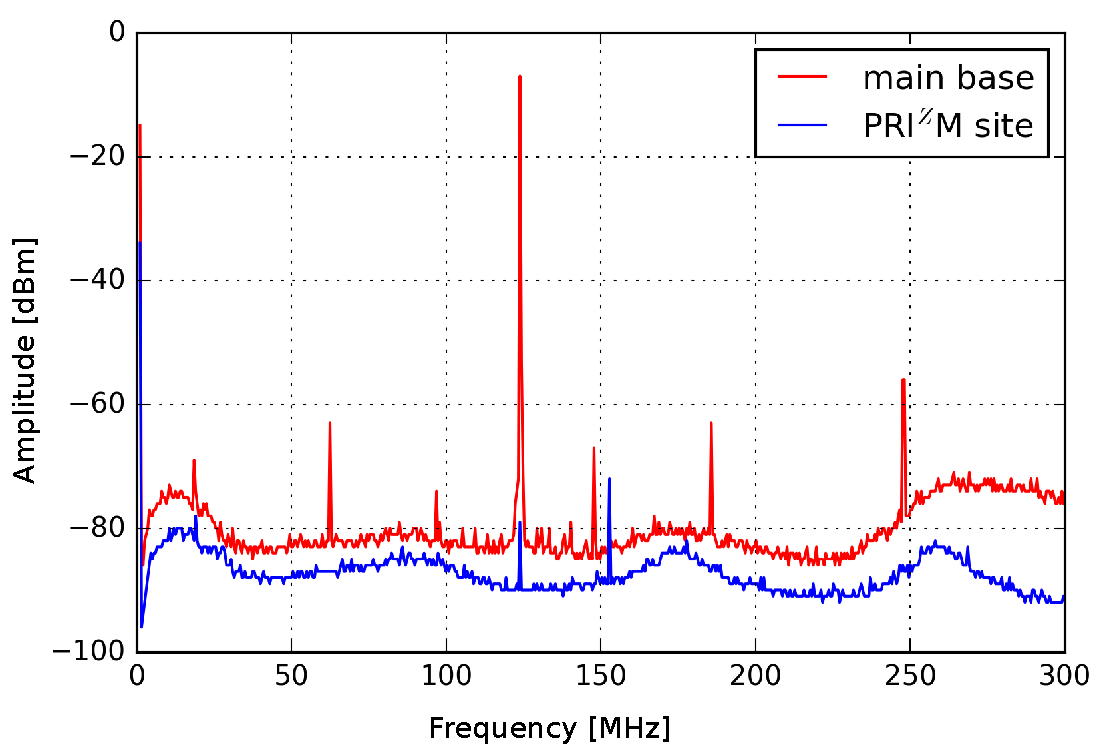
\includegraphics[width=\linewidth]{Figures/rfi}
	\caption{RFI measurement differentiated from the Marion base and the \prizm observing site. When the measurements were taken, the spectrum analyzer was set to max hold, and the measurement period coincided with the helicopter's operation near the base and transmitting at \SI{123.45}{\mega\hertz}. A rough benchmark of $\sim$60 dB signal suppression in received power at both locations arising from a combination of attenuation from Junior's kop and the distance between the \prizm site and the base. The peak at 156 MHz is a transmission from a handheld radio~\citep{2019JAI.....850004P}.}
	\label{fig:rfi}
\end{figure}

Figure~\ref{fig:IRI_model} shows the international reference ionosphere (IRI) model~\citep{ars-16-1-2018} predictions illustrating the minimum ionospheric plasma cutoff frequency during the last solar minima. The development of new low-frequency experiments is predominantly driven by the lack of knowledge of what lies in the sky at frequencies $\lessapprox$\SI{30}{\mega\hertz}.  According to the international reference ionospheric (IRI) model prediction, measurements of the sky at $\lessapprox$\SI{30}{\mega\hertz} do not look entirely impossible because, during the last solar \st{minima} \attention{minimum}, the ionospheric plasma cutoff frequency was \st{measured} \attention{predicted} to be $\sim$\SI{1.5}{\mega\hertz} at Marion Island. Since we are currently experiencing another solar minimum~\citep{2018NatCo...9.5209B}, it is an excellent opportunity to develop and implement new low-frequency observations. The prediction shows Marion Island, Dome C in Antarctica, and Hobart in Tasmania, where Reber performed his \SI{2}{\mega\hertz} observation. They have the potential to provide new views of the Earth's ionosphere, which absorbs and refracts at radio frequencies and becomes utterly opaque below the plasma cutoff frequency. \attention{[Since you've focused on the advantages of Marion, you may also want to include a couple of sentences about the drawbacks: limited access, Roaring 40s weather, mice, boundary conditions on equipment installs because it's an environmentally protected area, etc...but end on a positive note that although it's a somewhat steep price to pay, the reward is an unparalleled RF-quiet environment]} In the next two chapters, the \prizm\ and \albatros\ experiments are discussed in detail.

\begin{figure}
	\centering
	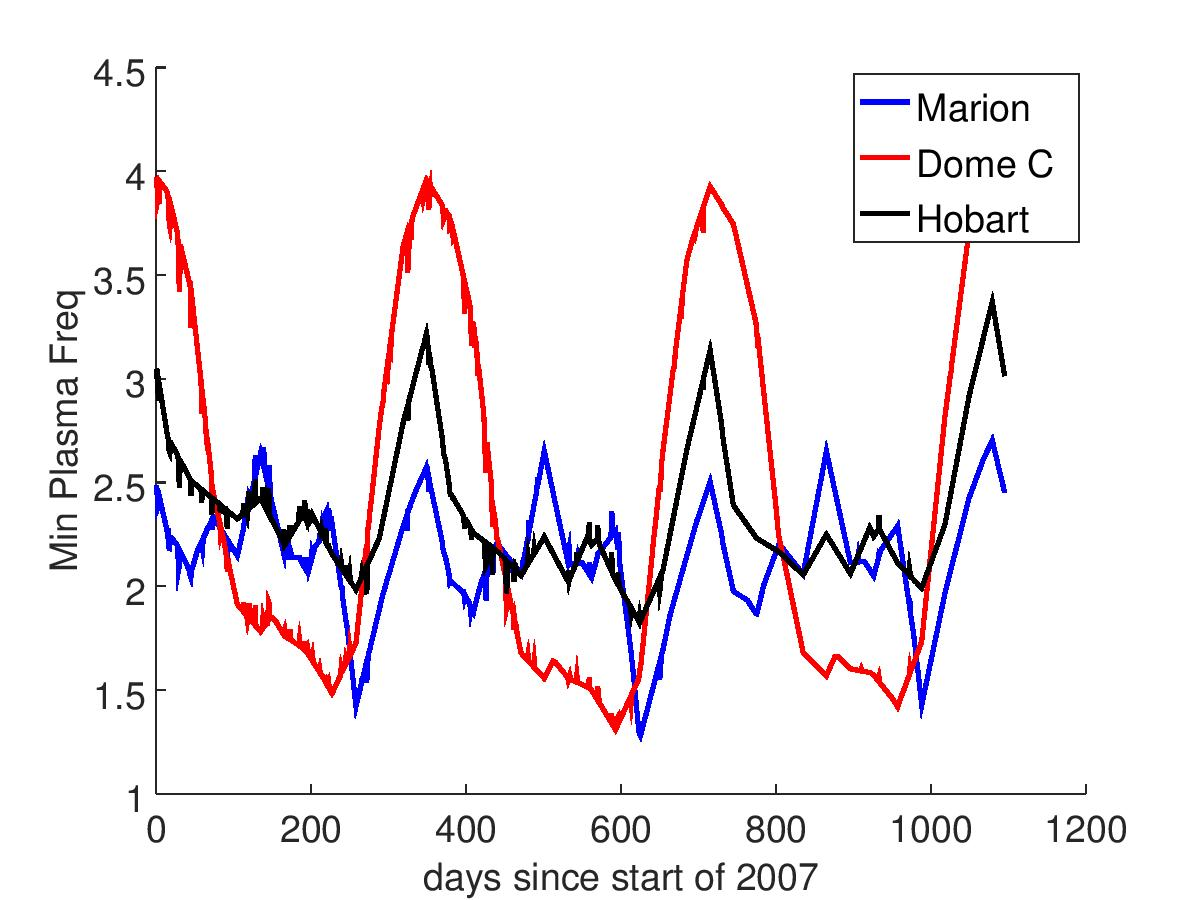
\includegraphics[width=\linewidth]{Figures/IRI_model}
	\caption{The International Reference Ionosphere model predictions illustrating the minimum ionospheric plasma cutoff frequency during last solar minima. At Marion Island, Dome C in Antarctica and Hobart in Tasmania the plasma frequency may drop as low as $\sim$\SI{1.5}{\mega\hertz}~\citep{2020arXiv200812208C}.}
	\label{fig:IRI_model}
\end{figure}

	\chapter{\albatros~Experiment}
\section{Overview of the Pathfinder}

\albatros~\citep[\albatros;][]{2020arXiv200812208C} pathfinder shown in Figure~\ref{Fig:albatros2} was introduced as an explorer in April 2018 at the \prizm\ site. Installing a pathfinder was a convenient way to assess Marion Island from discovering what is observable in the sky and finding out the observable frequencies. Figure~\ref{Fig:albatros2_schem} shows the block diagram of the pathfinder, and the signal chain description is below. The final experiment (\albatros) is aimed at consisting of autonomous antenna stations operating at a frequency range of \SIrange{1.2}{125}{\mega\hertz} that will map the low-frequency sky. Since these experiments are exploratory, they are taking steps towards achieving the future objective of coordinating observations to image the sky at frequencies that have been unexplored since the 1970s. These observations may allow us to probe even earlier epochs of the universe's history and will lay the groundwork for eventually exploring the cosmic "dark ages."

\begin{figure}
	\centering
	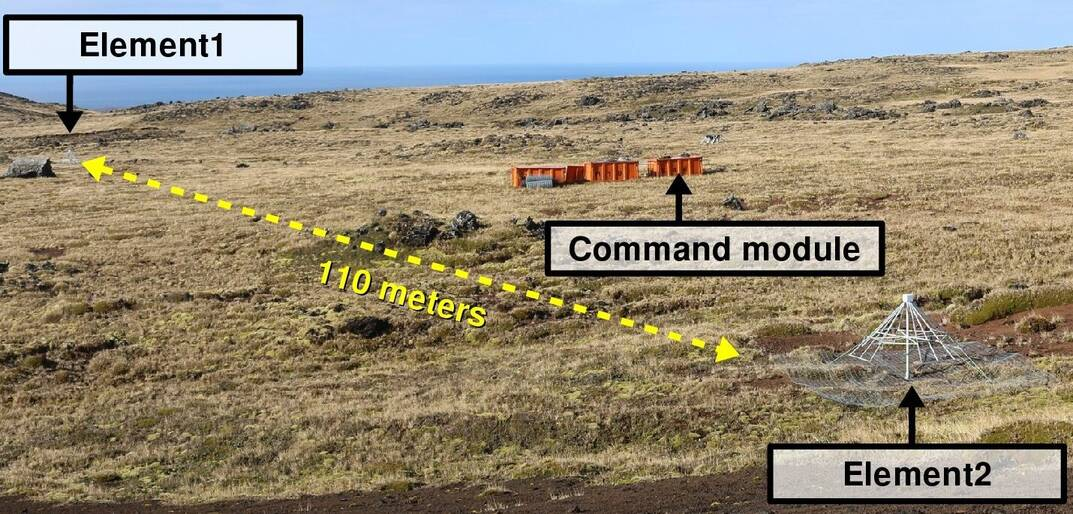
\includegraphics[width=\linewidth]{Figures/Albatros}
	\caption{The two-element, directly correlated \albatros\ pathfinder installed at the \prizm\ site. The pathfinder comprises two dual-polarization antennas separated by roughly 110 m on an east-west baseline. Coaxial cables connect the antennas to an orange shipping container that houses the readout electronics and serves as the "command module".}
	\label{Fig:albatros2}
\end{figure}

\section{Pathfinder System Signal Chain}

\begin{figure}
	\begin{center} 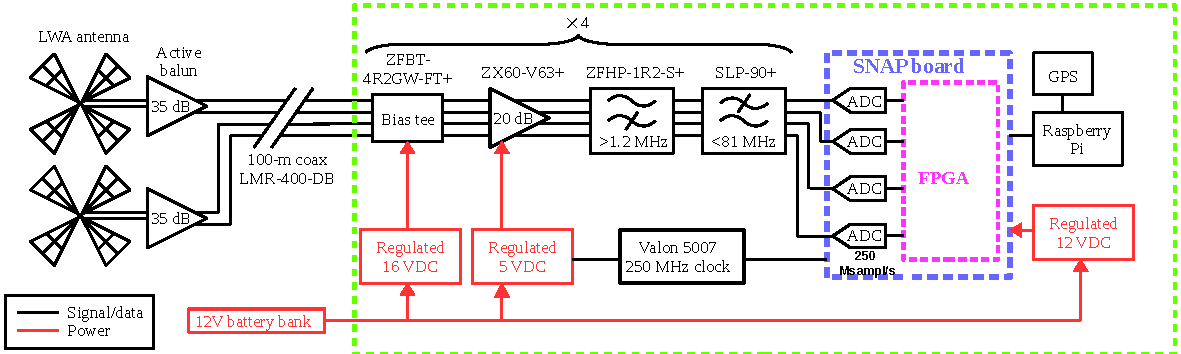
\includegraphics[width=\linewidth]{Figures/pathfinder_schematic.pdf}
		\caption{Two-element \albatros\ pathfinder block diagram.  Signals from two dual-polarzation LWA antennas are amplified by
			front-end active baluns~\citep{2012PASP..124.1090H}. The antennas are connected via 100-m coaxial cables to the back-end readout electronics, which are housed in a Faraday cage denoted by the green dashed box.  Each of the four antenna outputs is passed to a second-stage electronics chain consisting of filters and	further amplfication.  The signals are digitized at 250~Msamp/s by a SNAP board, which includes an on-board FPGA that computes auto- and cross-spectra from and between the four inputs.  A Raspberry Pi controls the SNAP board and saves the data.}
		\label{Fig:albatros2_schem}
	\end{center}
\end{figure}

\subsection{Antenna}\label{s:antenna}

The pathfinder uses two Long Wavelength Array (LWA) antennas configured as a two-element interferometric array. The two dual-polarization antennas are separated by $\sim$\SI{110}{\meter} on an east-west baseline. The dipole like antennas is of high preference for this project because they are relatively simple, and they are omnidirectionally patterned. The antennas possess low gain; therefore, the Galactic noise is limited by a fraction of 10, and the unwanted harmonics and intermodulation products are prevented~\citep{Memo28, Memo27}. The entire antenna and supporting structure sits on top of a ground screen that is roughly \SI{3}{\meter} on a side and is made of welded wire mesh.

\subsection{Front-end Electronics}\label{s:fee}

All the front end electronic (FEE) components are incorporated into a double-sided printed circuit board (PCB) as shown in Figure~\ref{Fig:balun} and the block diagram is shown in Figure~\ref{Fig:Balun Schematic}. One side of the PCB is populated with components, and the other side is a solid copper ground plane aperiodically stitched to the grounded copper on the side populated with components. The active balun provides an input impedance of \SI{50}{\ohm} to each dipole. The Mini-Circuits GALI-74+ monolithic microwave integrated circuit (MMIC) amplifiers from both feed points amplify each signal by +24 dB of gain. A passive {180\degree} hybrid coupler differentiates the two GALI-74+ outputs. A low-pass filters the coupler output by \SI{150}{\mega\hertz} and gains \SI{12}{\decibel} from the Mini-Circuits GALI-6+ MMIC. The signal gets fed to a second amplifier, and the output impedance of the FEE is matched to a \SI{50}{\ohm} \SI{100}{\meter} LMR400 coaxial cable having a nominal attenuation of $\sim$\SIrange{0.4}{3.7}{\decibel/100-m} at \SIrange{1.2}{81}{\mega\hertz}. The Mini-Circuits ZFBT-4R2GW-FT+ bias tee powers the FEE by \SI{16}{\volt} and extracts the RF signal by the use of the coaxial cable. The FEE has an overall gain of $\sim$ 36 dB and an overall noise figure of $\sim$ 2.7 dB to $\sim$ 2.9 dB~\citep{Memo35, 2012PASP..124.1090H}.

\begin{figure}
	\centering
	\begin{subfigure}[t]{0.52\textwidth}
		\centering
		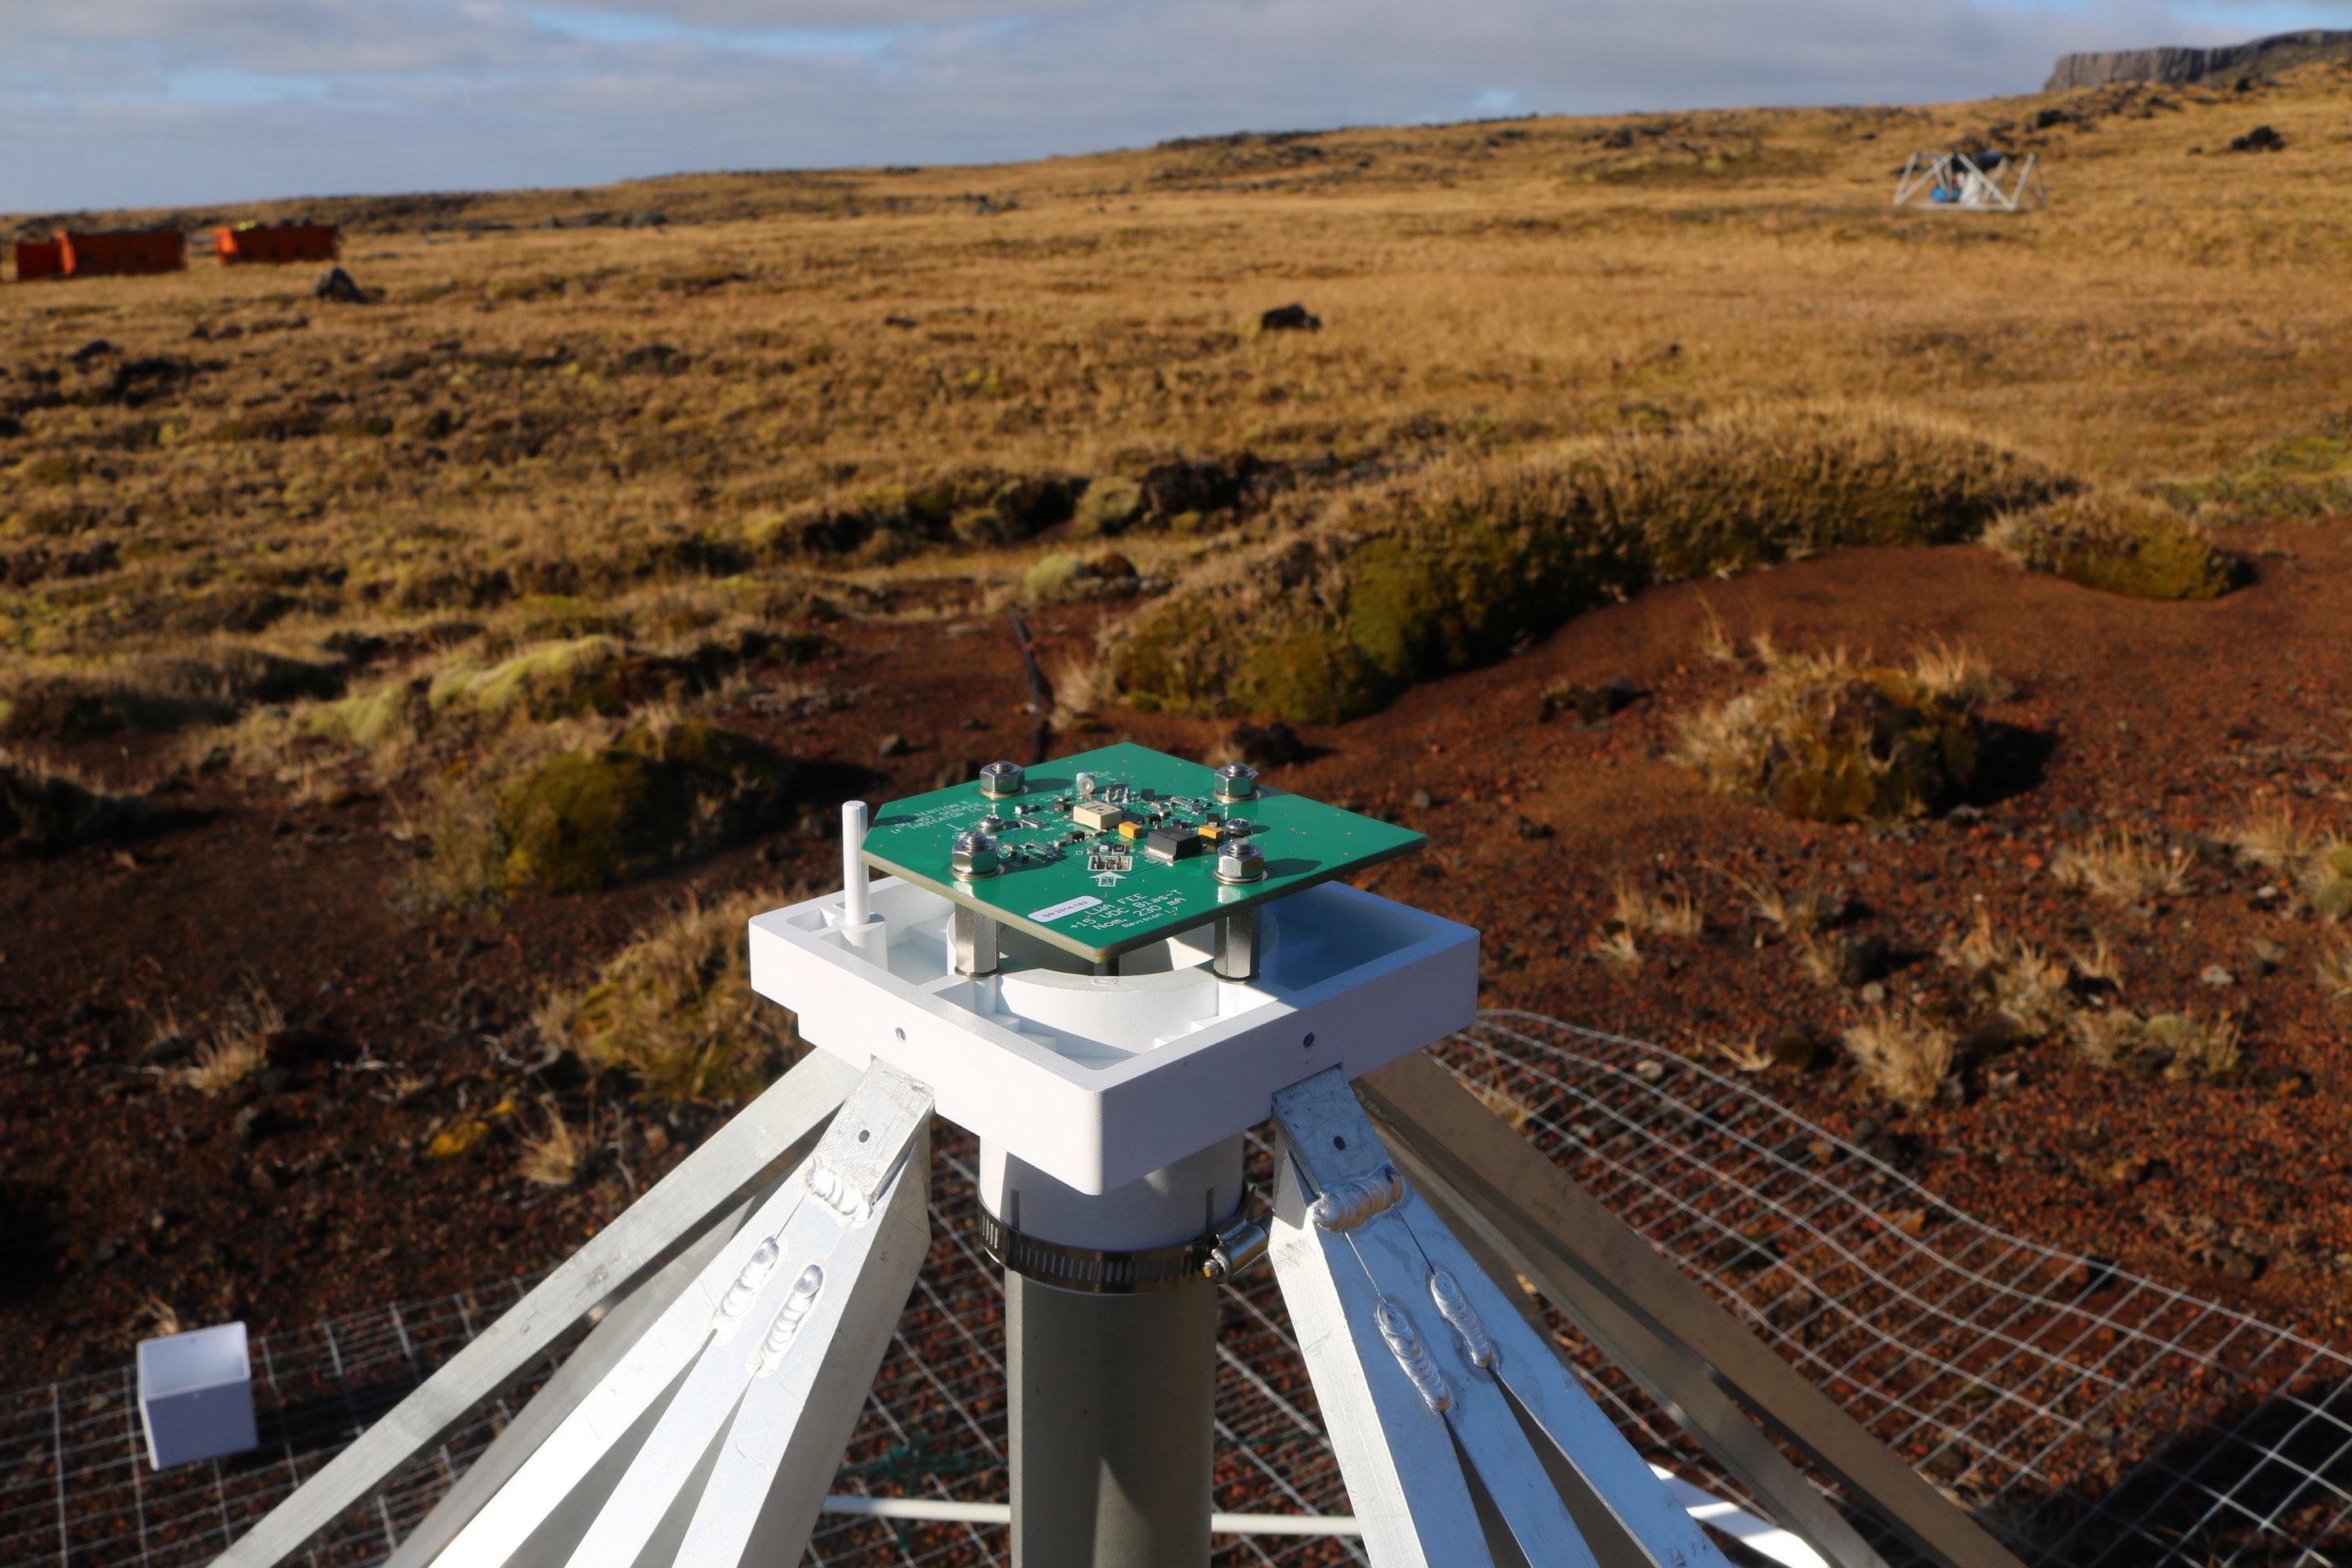
\includegraphics[width=\linewidth]{Figures/balun} 
		\caption{} \label{Fig:balun}
	\end{subfigure}
	\hfill
	\begin{subfigure}[t]{0.47\textwidth}
		\centering
		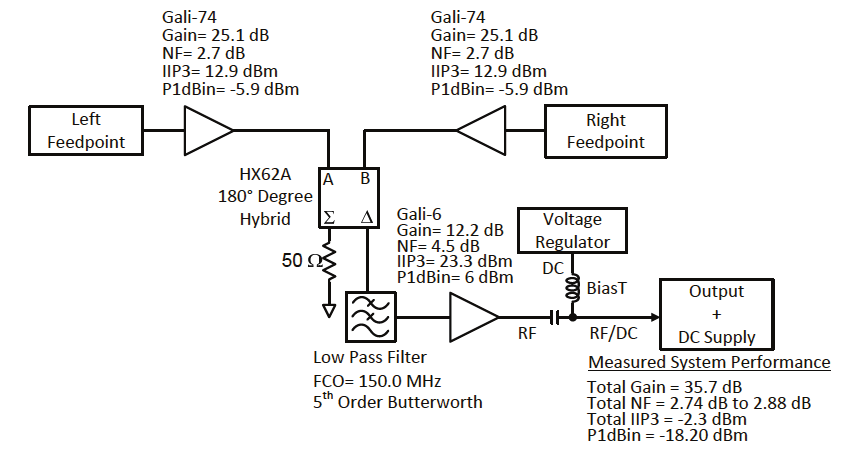
\includegraphics[width=\linewidth]{Figures/Balun_Block.png}
		\caption{} \label{Fig:Balun Schematic}
	\end{subfigure}
	\caption{{\bf (a)} Unenclosed FEE mounted on the pathfinder antenna supporting structure with the electronic components visible on the top part of the PCB. {\bf (b)} One Polarisation Block Diagram of the FEE \cite{2012PASP..124.1090H}} \label{Fig:fee}
\end{figure}

\subsection{Back-end Electronics}

The back-end electronics are housed in the Faraday cage shown in Figure~\ref{Fig:47093126504_fa0061a85b_o} denoted by the green dotted line box in Figure~\ref{Fig:albatros2_schem}. The analog signal chain consists of a Mini-Circuits ZX60-V63+ amplifier with a \SI{20}{\decibel} gain, and a pair of high- and low-pass filters (Mini-Circuits ZFHP-1R2+ and SLP-90+) that together band-limits the signal to \SIrange{1.2}{81}{\mega\hertz}. The amplifier operates at a frequency range of \SI{50}{\mega\hertz} - \SI{6}{\giga\hertz} and has a noise figure of $\sim$ 3.6 dB at its lowest operating frequency of \SI{\sim 50}{MHz}. The high- and low-pass filters present a nominal insertion loss of 0.2 dB and 0.14 dB at the center frequency of \SI{\sim10}{MHz}, respectively. 

\begin{figure}
	\centering
	\begin{subfigure}[t]{0.52\textwidth}
		\centering
		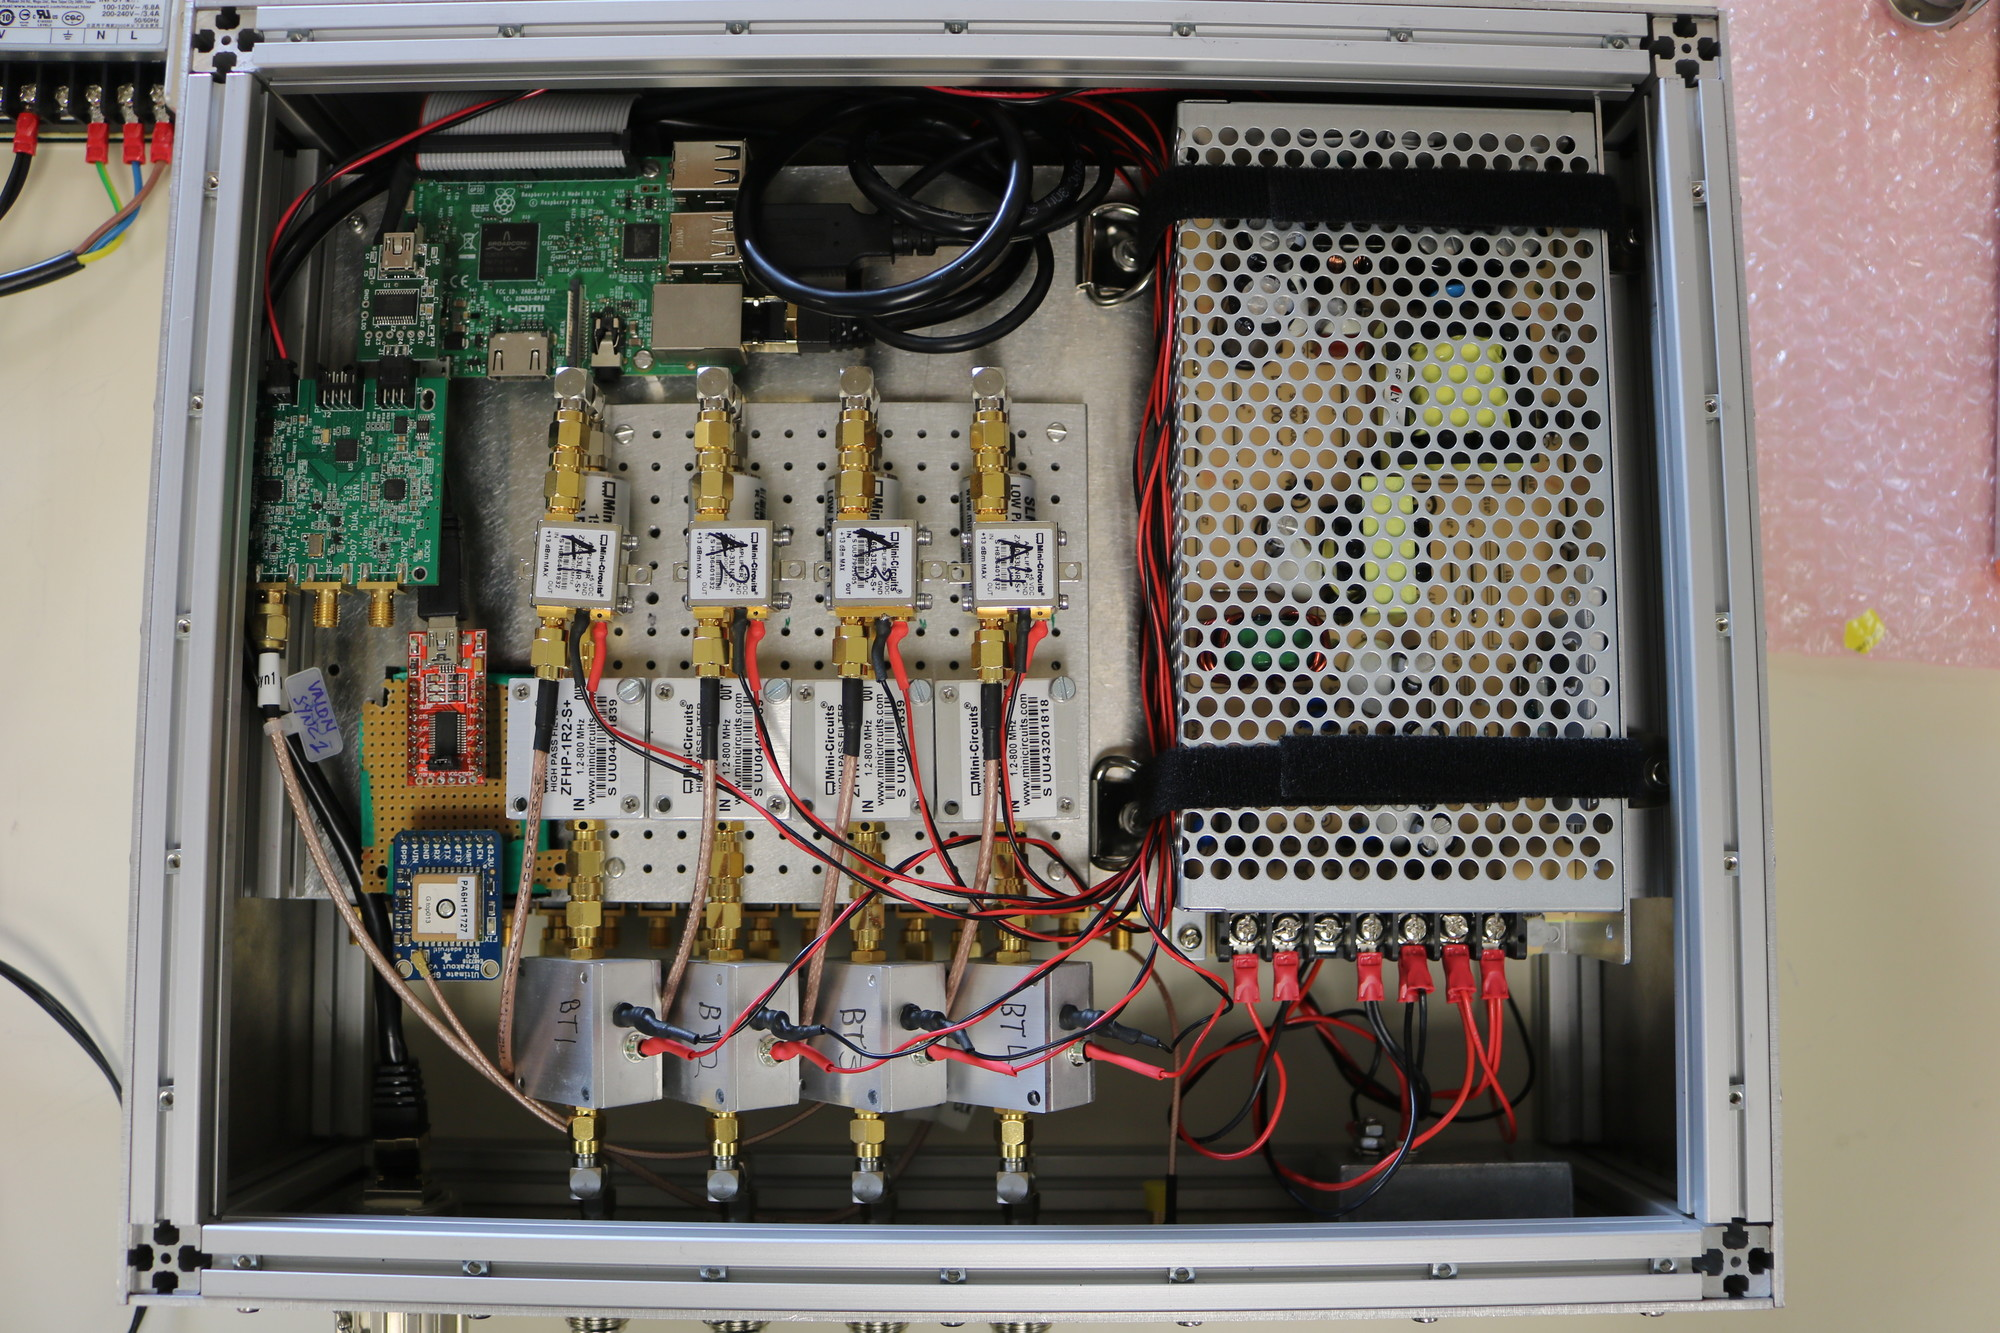
\includegraphics[width=\linewidth]{Figures/47093126504_fa0061a85b_o} 
		\caption{} \label{Fig:47093126504_fa0061a85b_o}
	\end{subfigure}
	\hfill
	\begin{subfigure}[t]{0.47\textwidth}
		\centering
		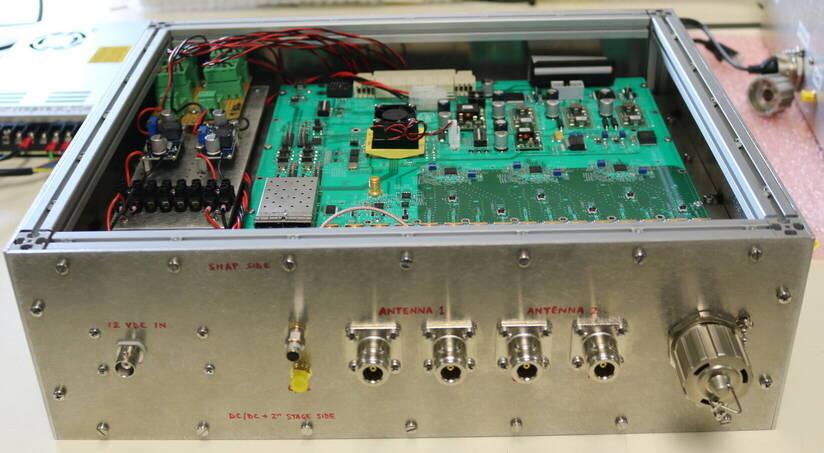
\includegraphics[width=\linewidth]{Figures/47093128324_04792aa5c5_o}
		\caption{} \label{Fig:47093128324_04792aa5c5_o}
	\end{subfigure}
	\caption{{\bf (a)} \albatros\ back-end electronics housed in the Faraday cage. One side of the mounting plate shows the amplifiers, pair of high- and low-pass filters, bias-tees, Valon 5007 frequency synthesizer module, RPi and Adafruit Ultimate GPS module. Component not visible on this side are mounted on the other side of the mounting plate. {\bf (b)} The bottom side of the \albatros\ Faraday cage, showing the mounted SNAP board and the regulatory circuit.} \label{Fig:faraday1}
\end{figure}

A Smart Network ADC Processor~\citep[SNAP;][]{2016JAI.....541001H} mounted in the Faraday cage in Figure~\ref{Fig:47093128324_04792aa5c5_o} samples the signals it receives by \SI{250}{Msampl/s} using an internal analog to digital converters (ADCs), and the signals of the clock are from the Valon 5007 frequency synthesizer module. A frequency range between \SIrange{0}{125}{\mega\hertz} containing 2048 channels is created by the SNAP board, which also includes the onboard Xilinx Kintex~7\footnote{\url{http://www.xilinx.com/products/silicon-devices/fpga/kintex-7.html}} FPGA that computes auto and cross spectra from and between the four inputs. A Raspberry Pi (RPi) controls the SNAP board and saves data to an onboard SD-card. The RPi absolute timing is provided by Adafruit Ultimate GPS module\footnote{\url{https://www.adafruit.com/product/746}}, connected
to an active external GPS antenna.

\subsection{Power}
The two-element pathfinder system is powered using four \SI{12}{\volt} \SI{200}{\ampere\hour} battery bank wired in parallel and battery charging is performed manually using a Honda EU30is\footnote {\url{http://www.hondaenergy.com/generators/honda-eu30is.html}} generator and a fuel cache that is kept at the observing site. The main advantage and encouragement to use a SNAP board is its low power consumption, which is feasible for the power supply method. The total system power draw is \SI{\sim45}{\watt} and the pathfinder system can operate without interruption for $\sim$1 week when the batteries are fully charged. During observations, the batteries are connected to DC/DC converters powering the SNAP board, FEE, amplifiers, and the clock. The DC-DC converters are housed inside the Faraday cage and provide stable voltage outputs	despite the slow decline of the battery voltage.

\section{Overview of Autonomous Stations}

The final ALBATROS array will consist of ten autonomous antenna stations (huts) separated by baselines of \SI{\sim {20}}{km} as shown in \autoref{Fig:marion_map}. Marion Island huts, which are potential stations for the ALBATROS array, have a ring-like pattern which is appropriate for imaging and produces an FWHM synthesized beam of $7'$ at \SI{5}{\mega\hertz} as shown in \ref{Fig:marion_map_beam}. The array beam promises an improved resolution over existing measurements to date. Thus far, the ALBATROS main goal will be to map high resolutions at low frequencies, which is crucial before doing cosmological observations of the dark ages. 

In April 2019, I was part of the deployment team in Marion Island, and I am going to discuss in detail the tasks associated with \albatros\ that we managed to complete during the three weeks relief voyage.  

\begin{figure}
	\centering
	\begin{subfigure}[t]{0.6\textwidth}
		\centering
		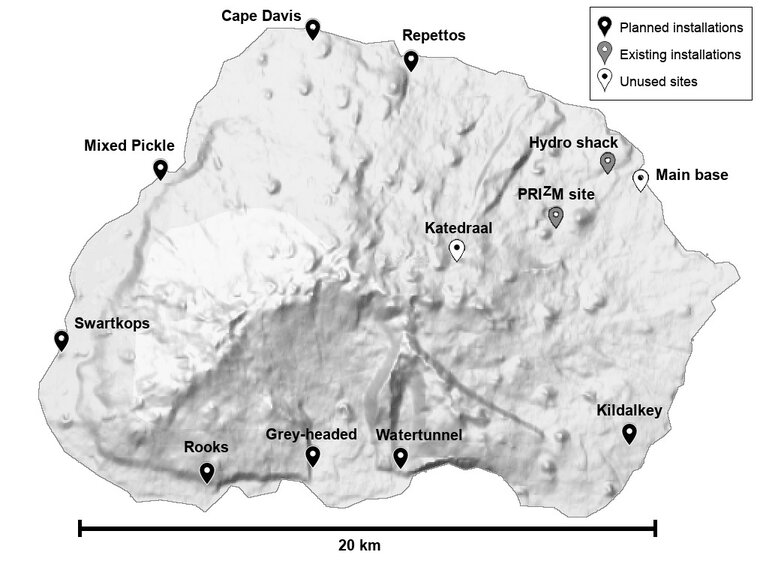
\includegraphics[width=\linewidth]{Figures/marion_map_annotated.jpg} 
		\caption{} \label{Fig:marion_map}
	\end{subfigure}
	\hfill
	\begin{subfigure}[t]{0.39\textwidth}
		\centering
		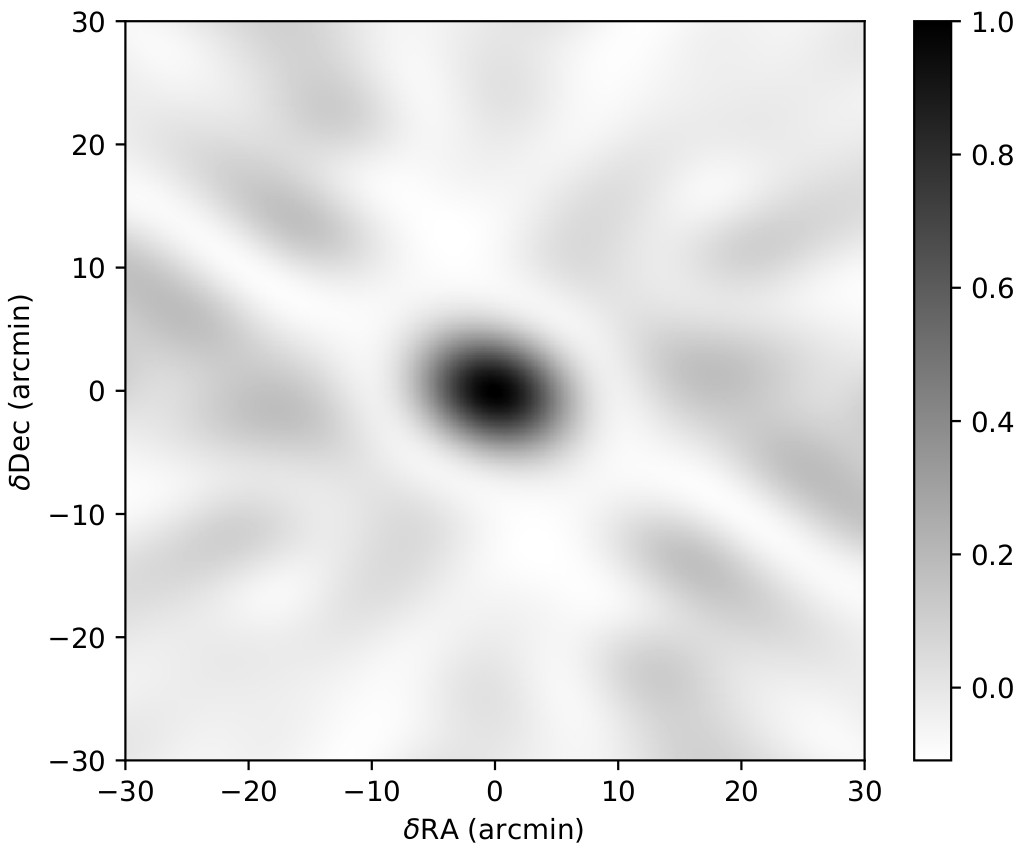
\includegraphics[width=\linewidth]{Figures/marion_beam_huts_2020.jpg}
		\caption{} \label{Fig:marion_beam}
	\end{subfigure}
	\caption{{\bf (a)} Map of Marion Island.  The
		\albatros\ pathfinder antennas are currently installed at the
		\prizm\ site and at the hydro shack (gray markers).  The black
		markers denote the eight coastal huts, which will be used for
		future \albatros\ antenna installations.  The white markers
		denote other available infrastructure points that will not be
		used for antennas. {\bf (b)} Synthesized beam at 5~MHz at zenith from the full \albatros\ array, using the existing and planned
		installation locations shown on the map.  Using an octave of
		bandwidth spanning 3.5--7~MHz in a single snapshot, we obtain a synthesized beam with a full width of $\sim7'$.}\label{Fig:marion_map_beam}
\end{figure}

\section{2019 Marion Voyage}

The S. A. Agulhas II sails from Cape Town each year in April. The relief voyage preparations begin months before the ship sails; the team plans and makes decisions based on the next voyage's goals. The development and testing of improved designs and systems occur at the University of KwaZulu Natal radio astronomy lab. In preparation for the 2019 voyage, I designed and developed a prototype solar power supply system that paved the way for the solar power supply system installed in Marion Island as part of the autonomous stations. Because of the weather conditions in Marion Island, the pathfinder system can shut down for an extended period without observations. Thus, a solar power system solution was implemented on the first autonomous station to run the system autonomously continuously. 

During the relief voyage, the installation process included mechanical assembly and alignment of the antenna structure itself, laying coaxial cables, installing three solar panel mounts (with three panels each, for a total of nine panels), and installing a small processing hub consisting of a plastic bin housing the readout electronics, two batteries, and power control electronics. The first autonomous station signal chain shown in Figure~\ref{Fig:albatros1_schem} was installed in April 2019 at the hydroshack site (\ang{46;52.205;}S, \ang{37;50.612;}E) on Marion Island as a first step in testing the technology needed to create the full array. A similar antenna and front end active balun discussed in (\S\ref{s:antenna} and \S\ref{s:fee}) were used, and the back-end electronics and the power system are discussed in detail below.

\section{Autonomous Stations Signal Chain}

\begin{figure}
	\begin{center}
		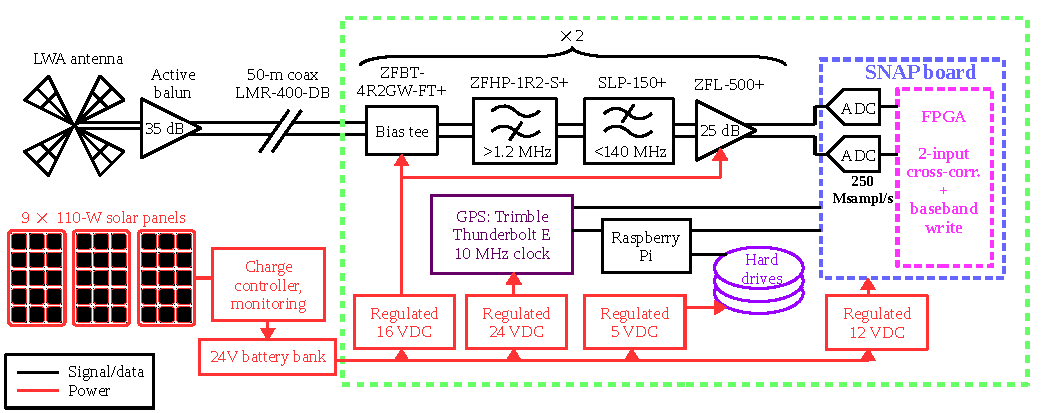
\includegraphics[width=\linewidth]{Figures/albatros_single_schematic.pdf}
		\caption{Single-antenna autonomous station block diagram. A dual-polarization LWA antenna, equipped with an active front-end balun, connects via 50-m coaxial cables to the back-end readout electronics, housed in a Faraday cage denoted by the green dashed box. Each of the two antenna signals is passed to a second-stage electronics chain consisting of filters and further amplification.  The signals are digitized at 250~Msamp/s by a SNAP board, including an onboard FPGA that computes channelized baseband and spectra from both inputs.  A Raspberry Pi controls the SNAP board and receives the baseband data and spectra. The baseband data are saved to external hard drives. The system is powered by solar panels that charge a 24-V battery bank.}
		\label{Fig:albatros1_schem}
	\end{center}
\end{figure}

\subsection{Back-end Electronics} 

\begin{figure}
	\begin{center}
		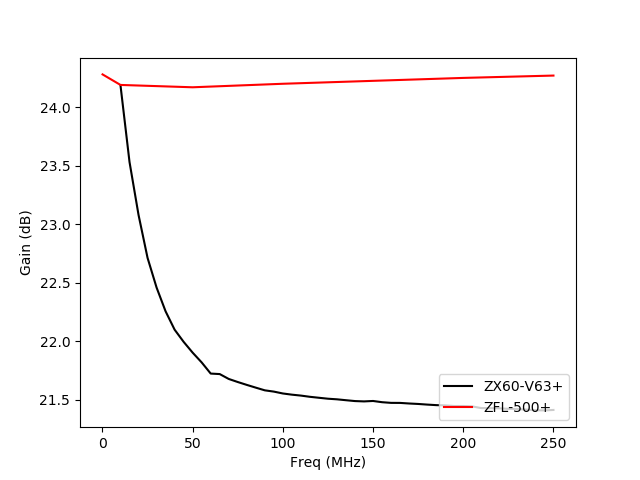
\includegraphics[width=0.8\linewidth]{Figures/foo.png}
		\caption{The comparison plot of S21 (gain) for the two-element pathfinder and the single autonomous station amplifier.}
		\label{Fig:foo}
	\end{center}
\end{figure}

\begin{figure}
	\centering
	\begin{subfigure}[t]{0.52\textwidth}
		\centering
		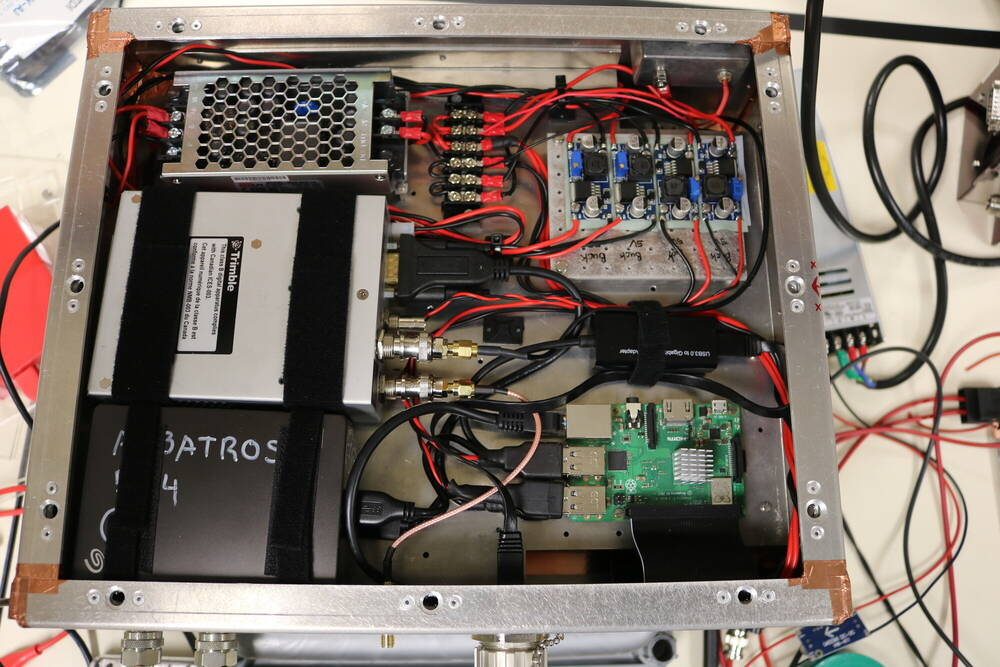
\includegraphics[width=\linewidth]{Figures/46966493985_44aa8ac326_o} 
		\caption{} \label{Fig:46966493985_44aa8ac326_o}
	\end{subfigure}
	\hfill
	\begin{subfigure}[t]{0.47\textwidth}
		\centering
		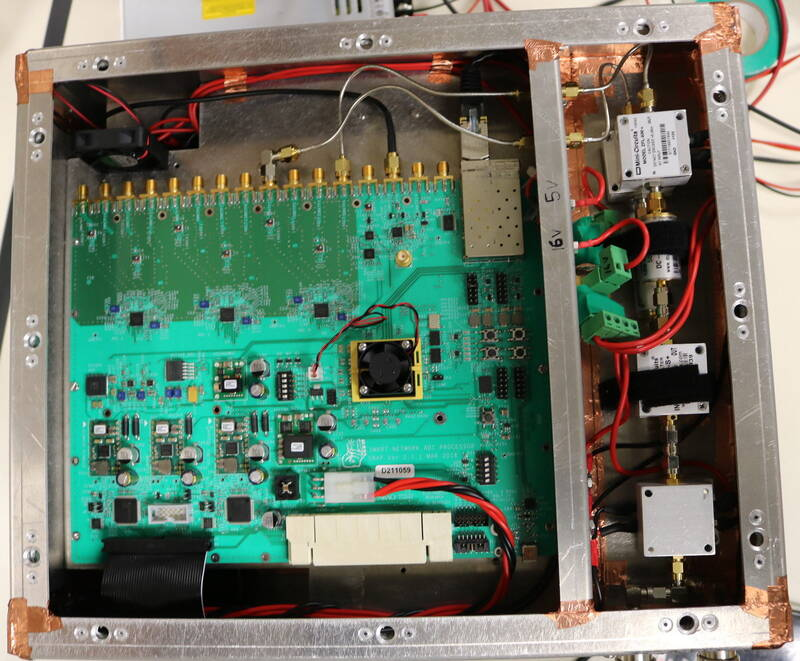
\includegraphics[width=\linewidth]{Figures/47882594521_3895effd86_o}
		\caption{} \label{Fig:47882594521_3895effd86_o}
	\end{subfigure}
	\caption{{\bf (a)} The single autonomous station Faraday cage showing one side of the mounting plate with visible power distribution circuitry, Trimble Thunderbolt E GPS-disciplined clock module, external hard drives and the RPi. {\bf (b)} The single autonomous station Faraday cage with the analog signal chain mounted in the RF partition on the left and the SNAP board mounted on the right.} \label{Fig:faraday}
\end{figure}

The Faraday cage shown in Figure~\ref{Fig:46966493985_44aa8ac326_o} denoted by the green dotted line box in Figure~\ref{Fig:albatros1_schem} is located \SI{50}{\meter} away from the antennas. The analog signal chain shown in Figure~\ref{Fig:47882594521_3895effd86_o} on the other side of the mounting plate in the RF partition consists of a pair of high- and low-pass filters (Mini-Circuits ZFHP-1R2+ and SLP-150+) that together band-limit the signal to \SIrange{1.2}{140}{\mega\hertz}, and after the filters is the Mini-Circuits ZFL-500+ amplifier with a \SI{25}{\decibel} typical gain. The amplifier operates at a frequency range of \SIrange{0.05}{500}{\mega\hertz}. Figure~\ref{Fig:foo} shows a comparison between the amplifier used on the two-element pathfinder and the single autonomous station. The plot shows an improved gain response; the ZFL-500+ amplifier response is flatter and is well within the experiment's operating frequency.

In comparison to the two-element pathfinder, the cut-off frequency of the low-pass filter increased from \SIrange{81}{140}{\mega\hertz} to capture downlink signals at \SIrange{137}{138}{\mega\hertz} from the ORBCOMM satellite constellation. The ORBCOMM signals are beneficial to the final \albatros\ array because they provide a convenient means for synchronization across the antenna stations, serving as a backup to the GPS timing discussed below. Actual lab tests recommend that on time scales of \SI{\sim 30}{\second}, relative timing between various autonomous stations can be estimated to a precision of better than a couple of tenths of a nanosecond utilizing a solitary satellite. At \SI{10}{\mega\hertz} the correlation phase error is $\lesssim1^\circ$. With open-access orbits and various satellites commonly within the field of view, the ORBCOMM baseband data supposedly saved simultaneously with the astronomical data can provide offline synchronization of the ALBATROS stations. Since the ORBCOMM and science data are recorded simultaneously by the same system, enhancement to the timing calibration can be applied in post-processing.

The signals are then digitized at \SI{250}{Msampl/s} by the SNAP board mounted in the Faraday cage in Figure~\ref{Fig:47882594521_3895effd86_o}. A Trimble Thunderbolt E GPS-disciplined clock module creates a \SI{10}{\mega\hertz} reference that is locked from the SNAP board internal ADCs. The SNAP board FPGA processes channelized baseband data for every polarization over tunable frequency windows inside the \SIrange{0}{125}{\mega\hertz} range, with the options of 1-, 2-, 4-bit baseband channelization, and auto-and cross-spectra from the two polarizations over the full \SIrange{0}{125}{\mega\hertz} range, collected more than few-second spans. The decrease in bit profundity happens simply after the SNAP board has channelized the baseband, and the cross-channel spillage (due to, e.g., RFI and inclines in RF power as observed by the ADCs) is thusly unaffected by the low bit profundity. 

An RPi 3B+ controls the SNAP board and gets the auto-and cross-spectra through GPIO pin connections, and the spectra are saved to an onboard SD card. The baseband data is passed through an ethernet from the SNAP board to the RPi and saved to external hard drives. The presentation of gigabit ethernet with the RPi 3B+ model has empowered the high data throughput related to writing baseband. As a benchmark, 1-bit baseband recording of two polarizations more than \SI{10}{\mega\hertz} of transmission capacity yields an inexact data rate of 5~MB/s or 400~GB/day.

\subsection{Correlation}

\subsection{Solar Power Supply System}

The future autonomous stations shown in Figure~\ref{Fig:marion_map} are farther from the island's main base; hence, the development of autonomous power supply systems. A solar power supply system was developed for the first autonomous station installed at the hydroshack site. The system is powered using an array of nine SunPower SPE-E-Flex-110 solar panels that charge a \SI{24}{\volt} battery bank made up of two series-connected, 12 V, deep cycle, lead-acid batteries. Each solar panel has a nominal power of \SI{110}{\watt}, capable of producing an open circuit voltage of approximately \SI{22.8}{\volt} and \SI{6.3}{\ampere}. On account of the extremely incessant cloudy conditions on Marion Island, the charging capacity of \SI{1}{\kilo\watt} is deliberately immense for the required \SI{\sim 50}{\watt} to run the station.

\begin{figure}
	\centering
	\begin{subfigure}[t]{0.52\textwidth}
		\centering
		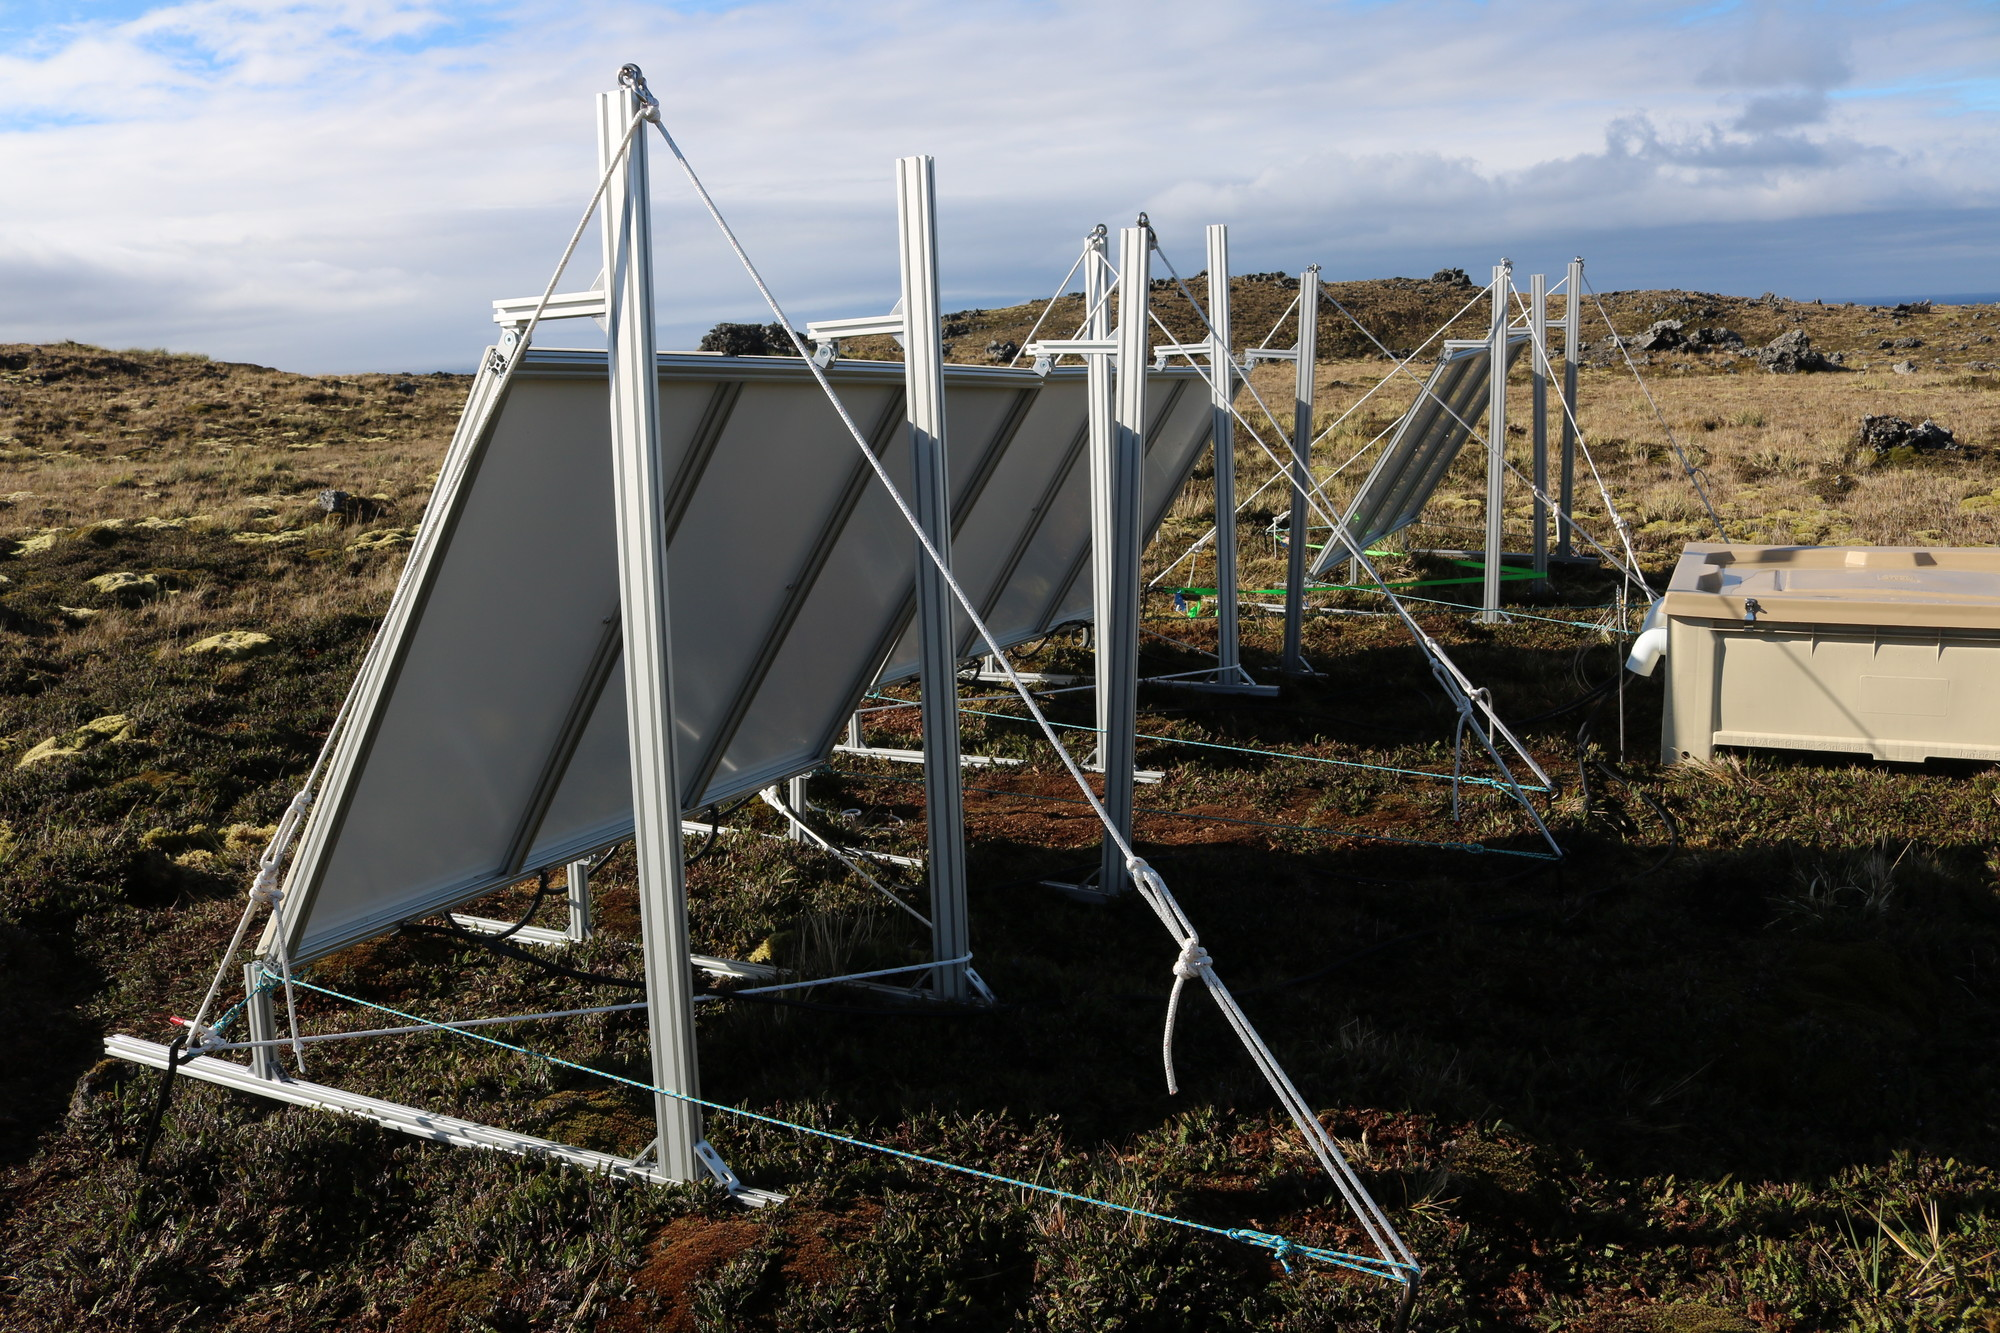
\includegraphics[width=\linewidth]{Figures/40916139043_f3d0c6b013_o} 
		\caption{} \label{Fig:40916139043_f3d0c6b013_o}
	\end{subfigure}
	\hfill
	\begin{subfigure}[t]{0.46\textwidth}
		\centering
		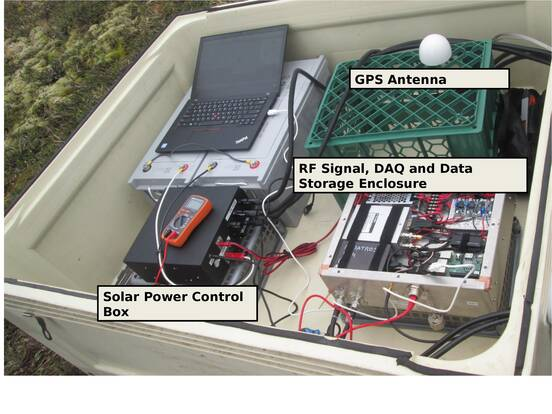
\includegraphics[width=\linewidth]{Figures/bin}
		\caption{} \label{Fig:bin}
	\end{subfigure}
	\caption{{\bf (a)} The three supporting structures for the nine solar panels mounted on a rigid metalized plastic panels. Behind the supporting structures is the plastic enclosure housing the readout electronics, two batteries, and the power control electronics. {\bf (b)} Interior of the  plastic enclosure housing the readout electronics, two batteries, GPS antenna, and the power control electronics} \label{Fig:power}
\end{figure}

The supporting structures for the nine solar panels were specifically designed to manage the gale-force winds on Marion Island, though it was challenging to install them as the volcanic ground minimizes the appropriate anchoring ability. The three aluminum mounting structures each carry three solar panels mounted on a rigid metalized plastic panel. The structures are oriented due north and are designed to incline the solar panels at a relatively steep angle to perform efficiently under winter conditions. The three supporting structures with mounted solar panels are shown in Figure~\ref{Fig:40916139043_f3d0c6b013_o}. Behind the supporting structures is the plastic enclosure housing the readout electronics, two batteries, and the power control electronics shown in Figure~\ref{Fig:bin}.

Each of the three solar panel sets is connected in series and parallel to the Victron BlueSolar MPPT 50|35 charge controller, optimizing power transfer from the solar array when charging is required, and monitors charge level reducing output current when the battery bank is fully charged. An Arduino logs the data from the Victron charge controller to an SD card and switches power on and off to the readout electronics box. The on/off feature is compulsory to avert battery system damage from excessively deep discharge. The system also has a battery power conservation feature, which schedules observations for distinct periods, often during the night when ionospheric conditions are more favorable. The power logging and control system, the Victron charge controller, and an EMI filter are housed together in an aluminum box shown in Figure~\ref{Fig:power_box_interior}. The solar charge controller generates RF noise, which would likely cause interferences; hence, an EMI filter was designed to minimize conducted emissions on the solar charge controller's photovoltaic side. Figure~\ref{Fig:station} shows the complete installation of the first autonomous station.

\begin{figure}
	\centering
	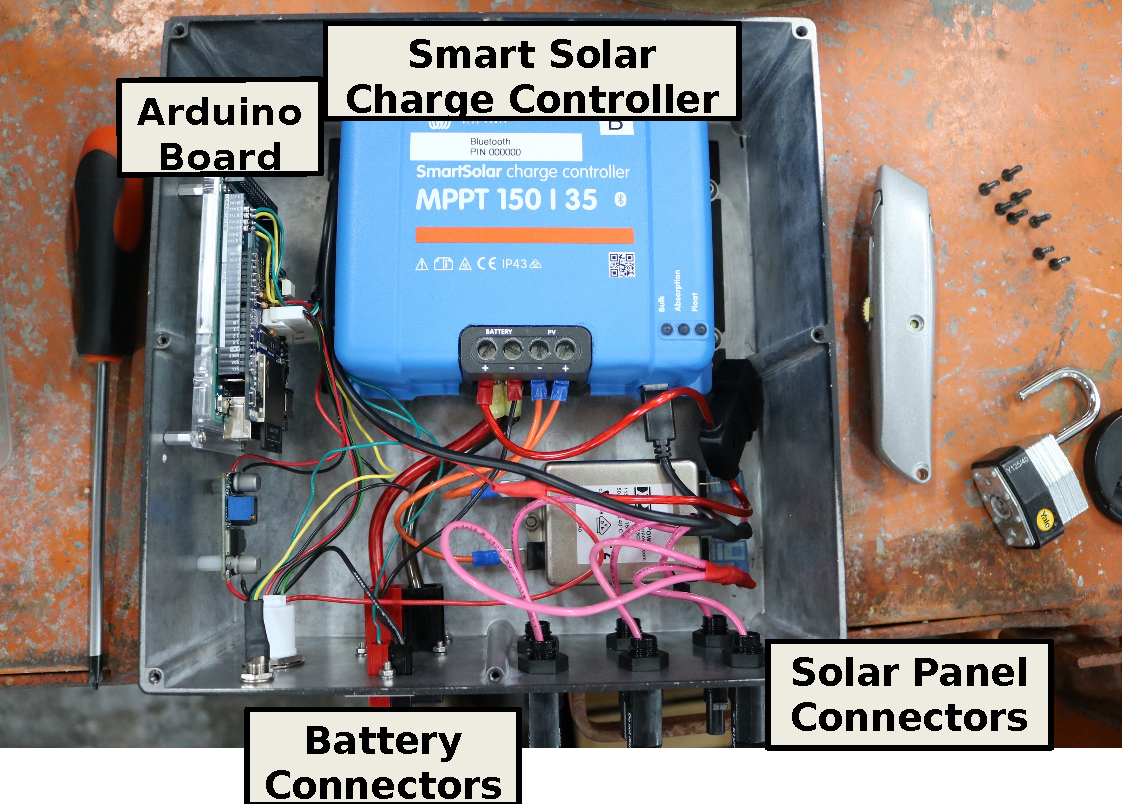
\includegraphics[width=\linewidth]{Figures/power_box_interior}
	\caption{The power logging and control system, the Victron charge controller, and an EMI filter are housed in an aluminum box.}
	\label{Fig:power_box_interior}
\end{figure}

\begin{figure}
	\centering
	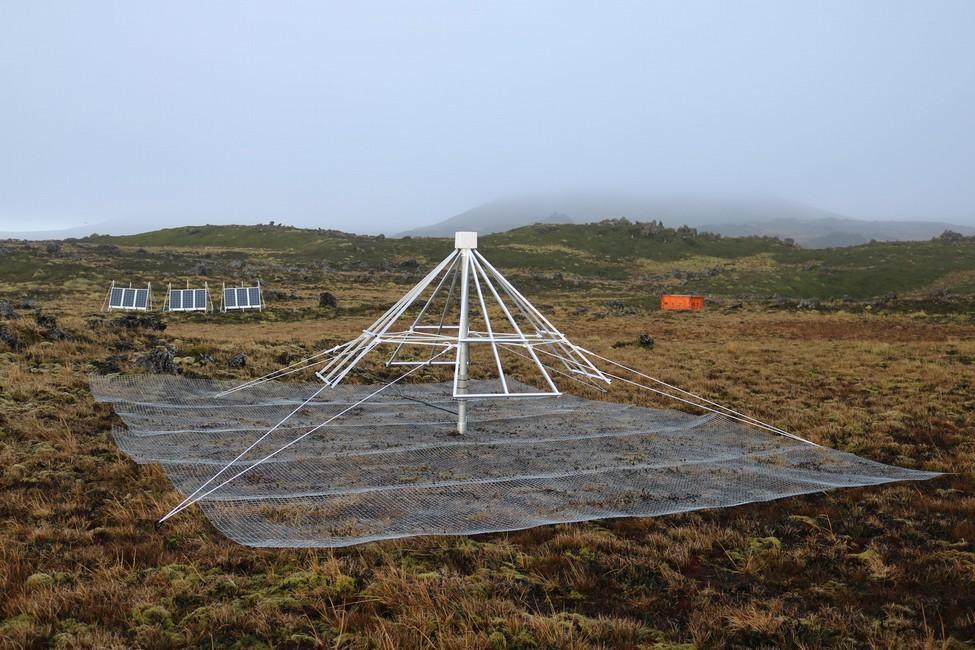
\includegraphics[width=\linewidth]{Figures/station}
	\caption{April 2019 deployment of the first \albatros\ autonomous station was a success. The mounted solar panels and the LWA antenna are visible.}
	\label{Fig:station}
\end{figure}

	\chapter{\prizm~Instrumentation}
\section{\prizm~Experiment Overview}

\prizm~\citep[]{2019JAI.....850004P} shown in Figure~\ref{Fig:prizm} is an experiment that is specifically designed to study cosmic dawn in the universe using total power measurements of the global 21 cm signal from neutral hydrogen, redshifted to \SIrange{30}{200}{\mega \hertz}. The experiment consists of two compact, modified four-square antennas \citep{8072391} that operate at central observing frequencies of 70 and 100~MHz. The combined frequency range of both antennas spans \SIrange{30}{200}{\mega \hertz}, which brackets the predicted absorption feature from cosmic dawn. Figure~\ref{Fig:PRZIM_block} shows the subsystems of \prizm\, which will be discussed briefly, followed by a discussion on revised subsystems. The first installation of \prizm\ in Marion Island was in 2017, and over the years, there have been incremental upgrades and maintenance to the front and back end electronics. My main contribution was making additional upgrades that were planned to field during the 2020 Marion takeover voyage, which unfortunately did not happen because of the COVID-19 restrictions.

\begin{figure}
	\centering
	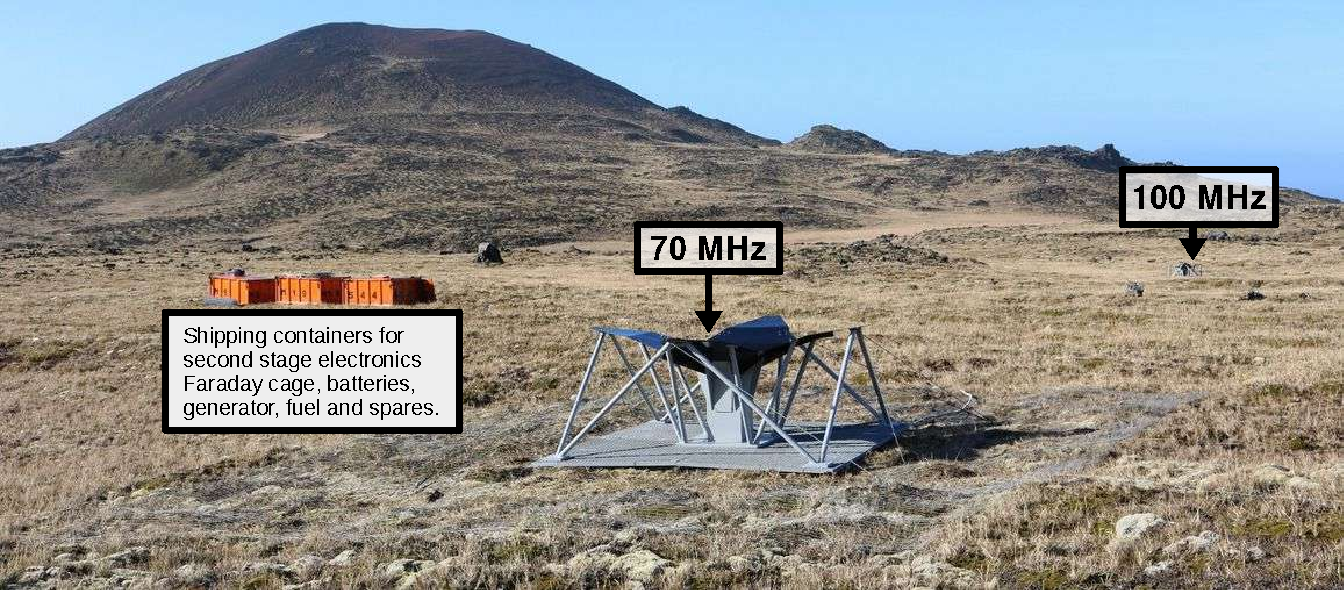
\includegraphics[width=\linewidth]{Figures/prizm.pdf}
	\caption{The \prizm\ experiment built on Marion Island. The two antennas (\SI{70}{\mega \hertz} and \SI{100}{\mega \hertz}) are visible and the the three shipping containers enclose the second stage electronics Faraday cage, generator, batteries, fuel, and spares. The main base lies four kilometers away from the observing site.}
	\label{Fig:prizm}
\end{figure}

\begin{figure}
	\centering
	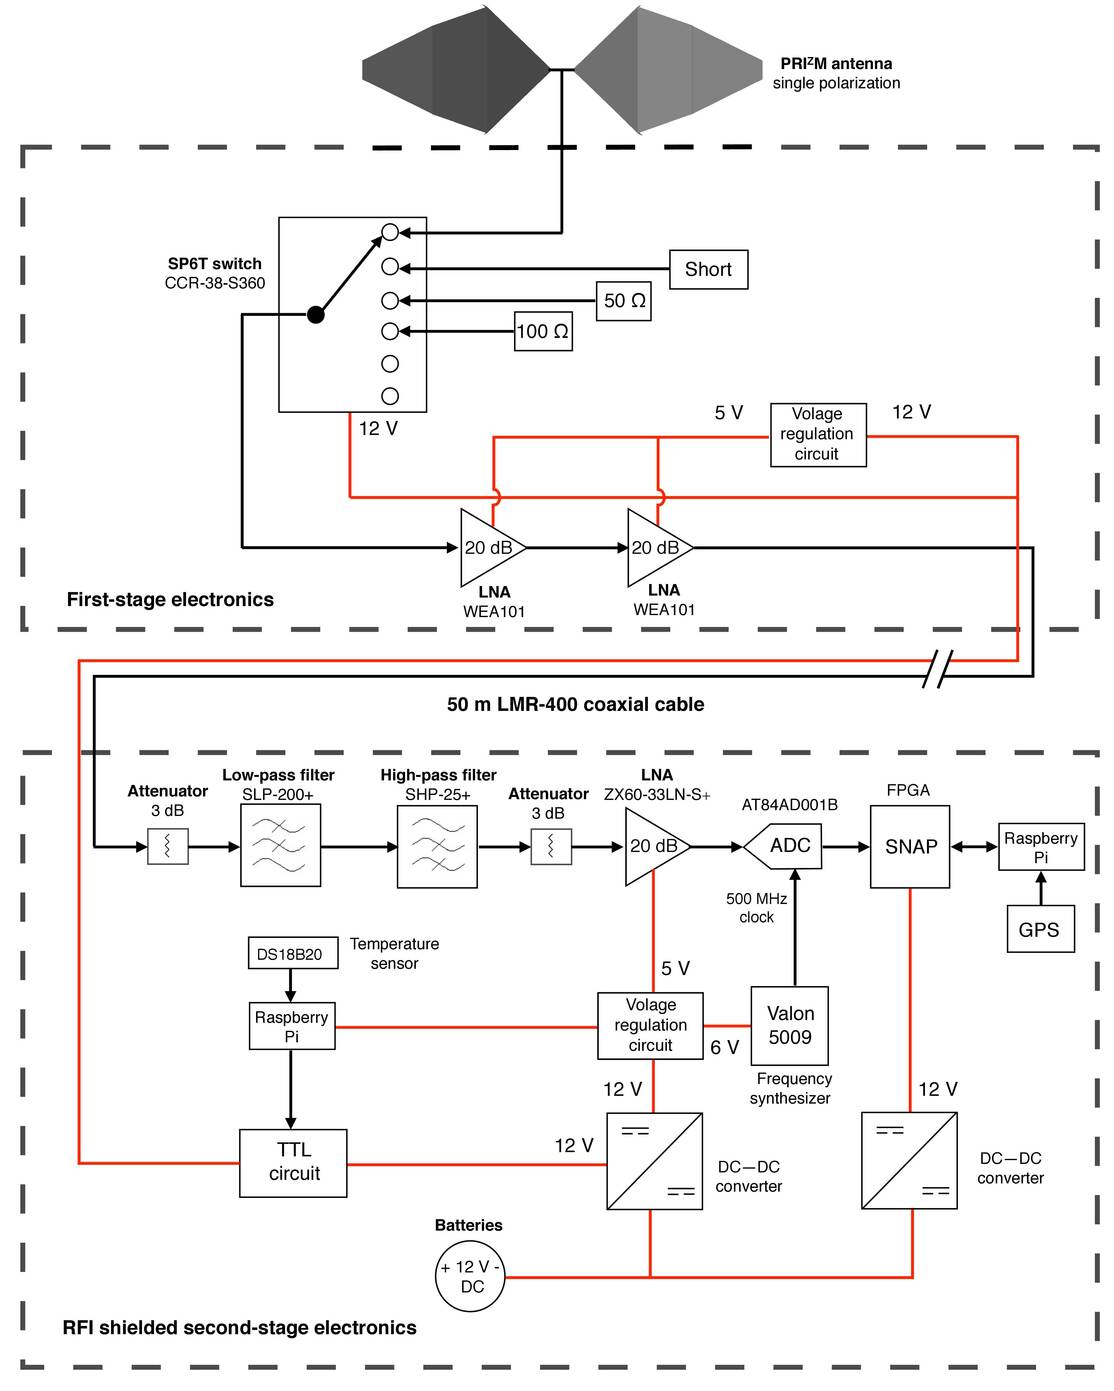
\includegraphics[width=\linewidth]{Figures/block_diagram}
	\caption{Block diagram for a single \prizm\ antenna polarization. The upper and lower dashed boxes denote the electronics chain's first and second stages. To decrease contamination from self-generated RFI, the 
		two stages are separated by \SI{50}{\meter}~\citep{2019JAI.....850004P}}. 
	\label{Fig:PRZIM_block}
\end{figure}

\section{Signal Chain}

\subsection{Antenna}

Figure~\ref{Fig:PRZIM_block} shows the original 2017 configuration of the signal chain for a single polarization of the \prizm\ antenna. The antenna design was initially developed for Sonda Cosmologica de las Islas para la deteccion de HIdrogeno neutro (SCI-HI), which was deployed in Guadalupe Island (\SI{200}{\kilo \meter} off the coast of Mexico) in 2013. The antenna is made up of four petals that form a pair of crossed dipoles. 

Each petal has three trapezoidal facets angled at various angles with respect to the ground. The angles were selected to minimize spectral variation in the beam shape. The antenna beam pattern's width has a direct dependence on the angles of the trapezoidal facets, and the height of the antenna above the ground changes the beam symmetry~\citep{2014ApJ...782L...9V}.  The \prizm\ antenna structure was redesigned with respect to the original SCI-HI design to survive the high winds on Marion Island, as shown in Figure~\ref{Fig:tel}.  


\begin{figure}
	\centering
	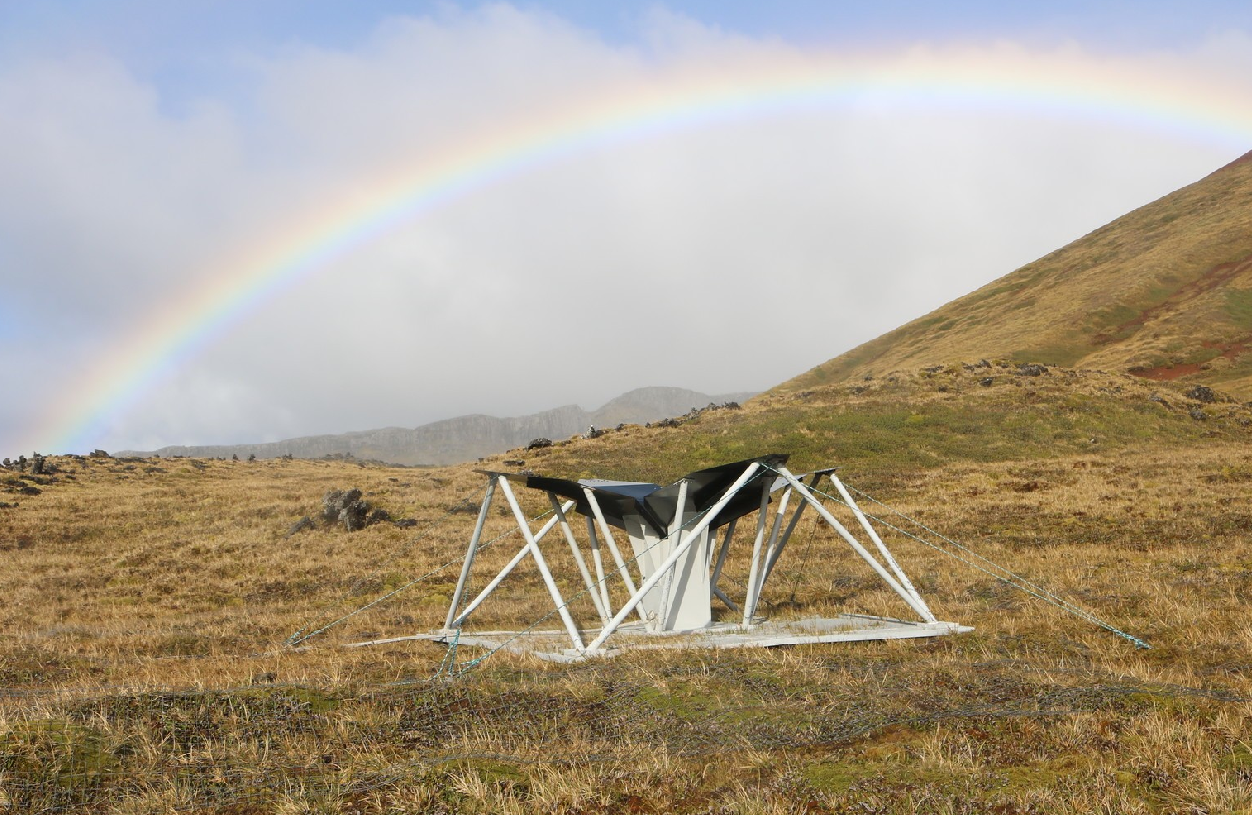
\includegraphics[width=\linewidth]{Figures/tel}
	\caption{A completed \SI{100}{\mega \hertz} antenna mounted on a \SI{2x2}{\meter} fibreglass grating with the approximate dimensions \SI{\sim 3}{\meter} on a side}.
	\label{Fig:tel}
\end{figure}

\subsection{First Stage Electronics}

The first stage electronics are housed in the column supporting the antenna petals as shown in Figure~\ref{Fig:column}, and the block diagram of the first stage electronics is shown in Figure~\ref{Fig:prizm_fee_block}. The signal from each single-polarization \prizm\ dipole is fed to the calibrator switch by a coaxial cable, which is \SI{200}{\milli \meter} long. In order to dissipate the current on the outer conductor of the coaxial cable, a ferrite core is used. The calibrator switch is required to switch between observations of the sky and the calibrator sources of \SI{50}{\ohm}, which are connected to the switch input terminals. Two cascaded WEA101 LNAs are used to amplify the selected signal at the switch output. Additional electronics in the first stage electronics box include voltage regulation circuitry for LNAs and temperature sensors. The two main improvements are upgrading to a latching switch from the 2017 to 2018 version, adding the noise source, and spreading thermometry through the components shown in Figure~\ref{Fig:prizm_fee_block}.

\begin{figure}
	\centering
	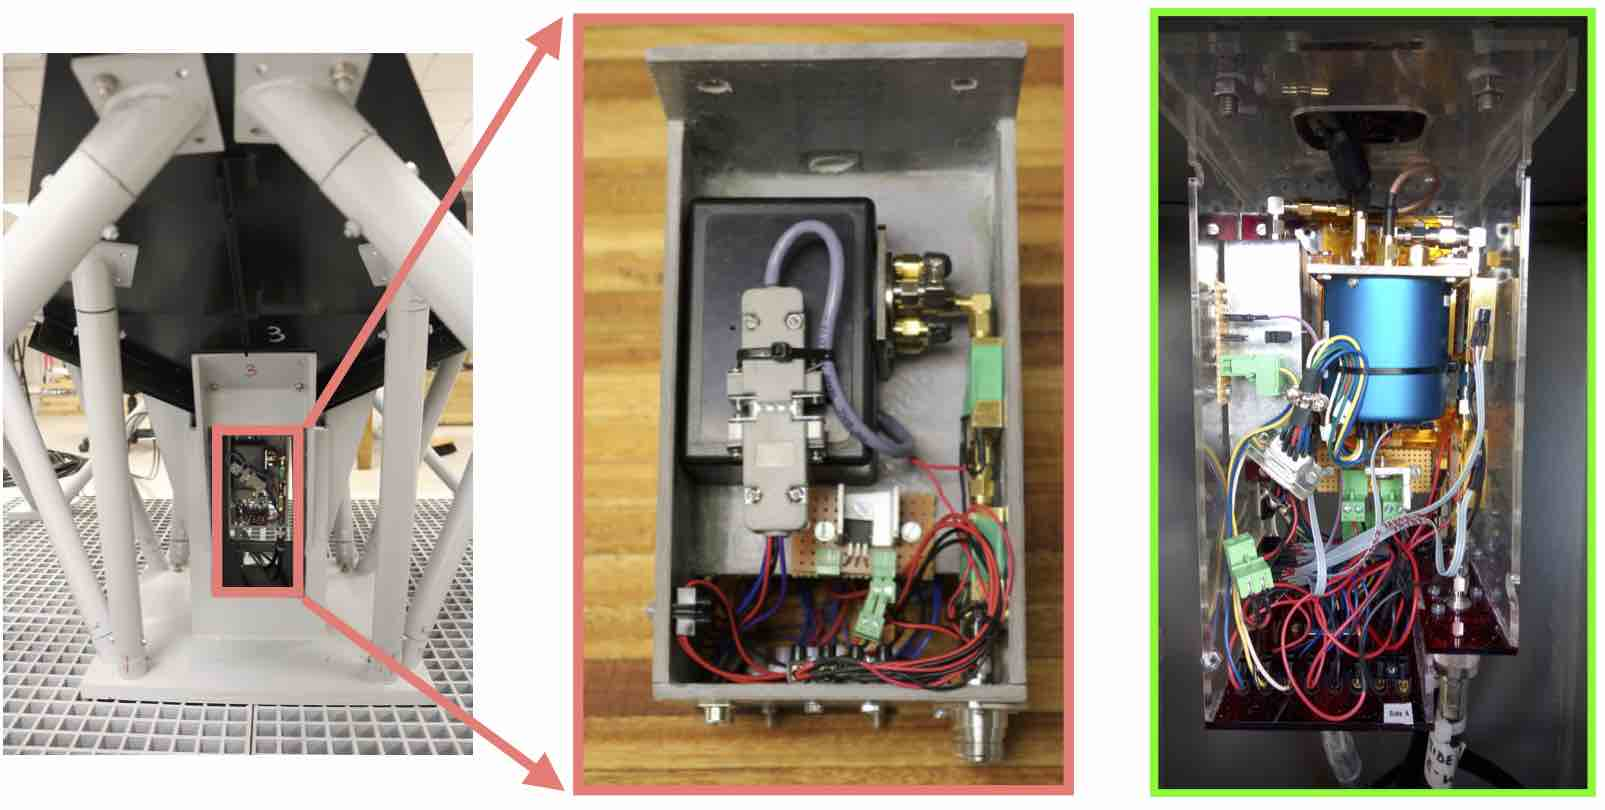
\includegraphics[width=0.7\linewidth]{Figures/column}
	\caption{The electronics box for the first stage. Shown in pink is the original installation from 2017 and green shows the 2018 upgrade which is currently installed in the central column under the antenna.}
	\label{Fig:column}
\end{figure}

\begin{figure}
	\centering
	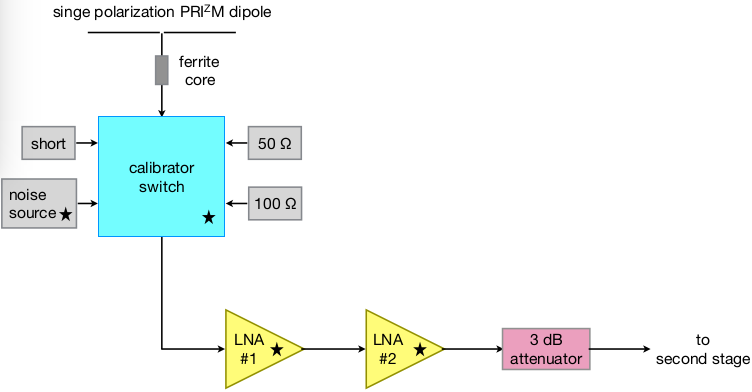
\includegraphics[width=\linewidth]{Figures/prizm_fee_block}
	\caption{A simplified schematic of electronics from the first stage. The schematic reflects the 2018 configuration. Components marked with a star are outfitted with one-wire digital temperature sensors.}
	\label{Fig:prizm_fee_block}
\end{figure}  

\subsection{Second Stage Electronics (SSE)}

A custom-designed Faraday cage (Figure~\ref{Fig:47093285614_63bb00be20_o}) that encloses the SSE is housed in one of the shipping containers shown in Figure~\ref{Fig:prizm}. The signal from the first stage electronics is fed via a \SI{\sim 50}{\meter} LMR400 coaxial cable, which is a reasonable distance to minimize the contamination from possible self-generated RFI. The coaxial cables are mouse-proofed using a few meters of stainless steel wire mesh cloth wrapped near the cable penetration points. The multi-tiered interior of the Faraday cage (\SI{\sim 300x470x240}{\milli \meter}) is shown in Figure~\ref{Fig:enclosure_ann} with the top panel removed. The readout box services both antennas. There is a separate readout chain for each antenna, but the housekeeping and switch control electronics are shared between the antennas. There are two central shelves for mounting the SNAP board and RPis. Each SNAP board services each antenna, and one RPi controls each SNAP. A third RPi is shared amongst the two SNAP boards for housekeeping purposes.

The filtering and amplification stage is applied to each polarization from each antenna. It consists of Minicircuits SLP-200+ and SHP-25+ low and high pass filters that band limit the RF signal to \SIrange{30}{200}{\mega \hertz}. The filtered signal is amplified by \SI{20}{\decibel} using a Minicircuits ZX60-33LN-S+ amplifier. The output signal is then fed to the readout electronics.

Each SNAP board receives the two RF signals from the two polarizations of a single antenna and samples the signals at a rate of \SI{500}{\mega samp\per \second} using a dual, monolithic, eight-bit, AT84AD001B external analog-to-digital converter (ADC) that is connected to the SNAP board via a Z-Dok connector. A Valon 5009 frequency synthesizer provides the ADC with a clock signal. The SNAP board employs a Xilinx Kintex 7 FPGA to compute auto- and cross- spectra from and between the four inputs, with 4096 frequency channels spanning 0--250~MHz. An RPi controls the SNAP board and saves data to an onboard SD-card. The RPi's timing is provided by an Adafruit Ultimate GPS module connected to an external active GPS antenna.

The SSE box also encloses the additional hardware that controls the calibrator switch states and voltage regulation. Figure~\ref{Fig:calibrator} shows the schematic of the switch control circuit. The L298 full-bridge drivers were used to make the control circuit, and the transistor-transistor-logic (TTL) is used to generate the control signals. Five L298 high-current full-bridge drivers are used to provide the reset and actuation signals. A power MOSFET is used to turn on and off a noise source in the FSE box. A Rpi controls the logic gates of the integrated chips. The whole first stage electronics is temperature monitored using the 1-wire DS18B20 temperature sensor.

\begin{figure}
	\centering
	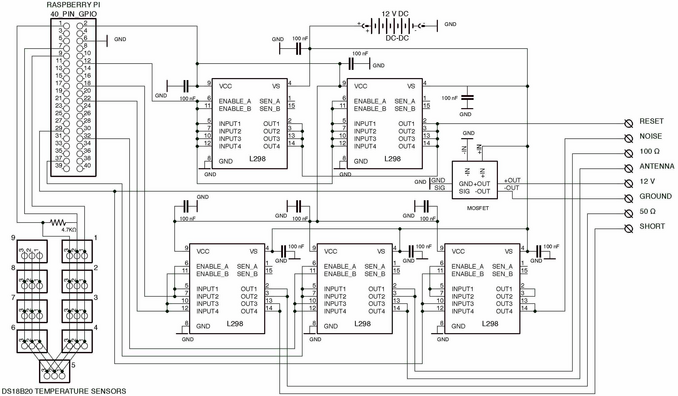
\includegraphics[width=\linewidth]{Figures/calibrator}
	\caption{The schematic of a switch control circuit. The L298 full-bridge drivers were used to make the control circuit. The two top drivers provide the reset signals, and the three bottom drivers provide actuation signals. To turn on and off the noise source in the FSE box, a power MOSFET is used. Nine 1-wire DS18B20 temperature sensors monitor the temperature.}
	\label{Fig:calibrator}
\end{figure}

The main power to the SSE box is fed via a BNC connector. The SSE box houses the two DC-DC converters on the bottom layer, which both provide \SI{12}{\volt} output, two SNAP boards are powered with \SI{12}{\volt} from one DC-DC converter. There are additional power regulators that input the \SI{12}{\volt} from the other DC-DC converter to supply lower voltage levels to multiple components in the system.

\begin{figure}
	\centering
	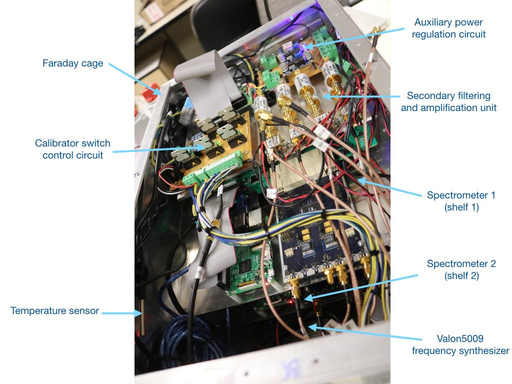
\includegraphics[width=0.7\linewidth]{Figures/enclosure_ann}
	\caption{The multi-tiered interior shown while the SSE box top panel is removed. Most of the internal components in this configuration can be accessed, but one more panel needs to be opened to access the DC-DC converters.}
	\label{Fig:enclosure_ann}
\end{figure}

\begin{figure}
	\centering
	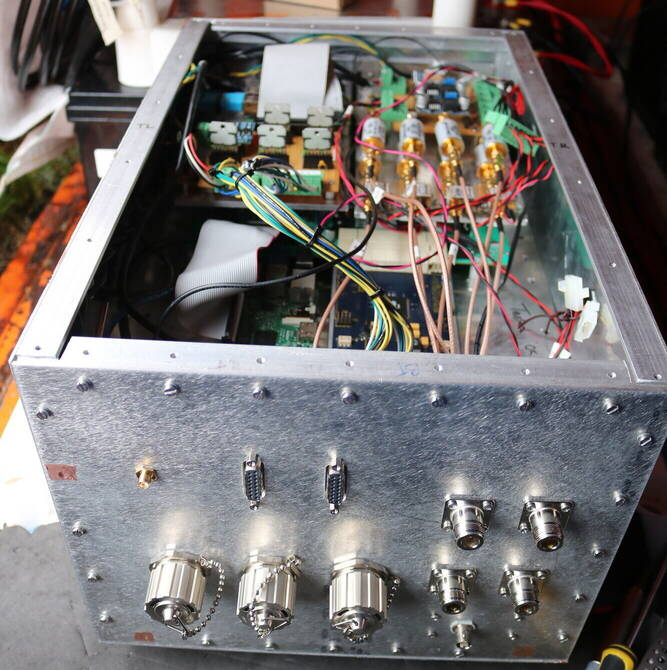
\includegraphics[width=0.4\linewidth]{Figures/47093285614_63bb00be20_o}
	\caption{The SSE Faraday cage made with separate brackets and flat sheets.}
	\label{Fig:47093285614_63bb00be20_o}
\end{figure}       

\subsection{Power}

The \prizm\ system is powered using eight \SI{12}{\volt} \SI{200}{\ampere \hour} battery bank wired in parallel as shown in Figure~\ref{Fig:power}. The total system draws \SI{\sim 65}{\watt} when the batteries are fully charged, the system can operate for approximately one week. Battery charging is performed manually using a Honda EU30is generator, and a fuel cache kept at the observing site. The batteries are connected to two DC/DC converters during observations. The DC-DC converters are enclosed in the SSE box and provides stable voltage outputs despite the slow decline of the battery voltage. Further regulation is performed to supply power to several components in the system.

\begin{figure}
	\centering
	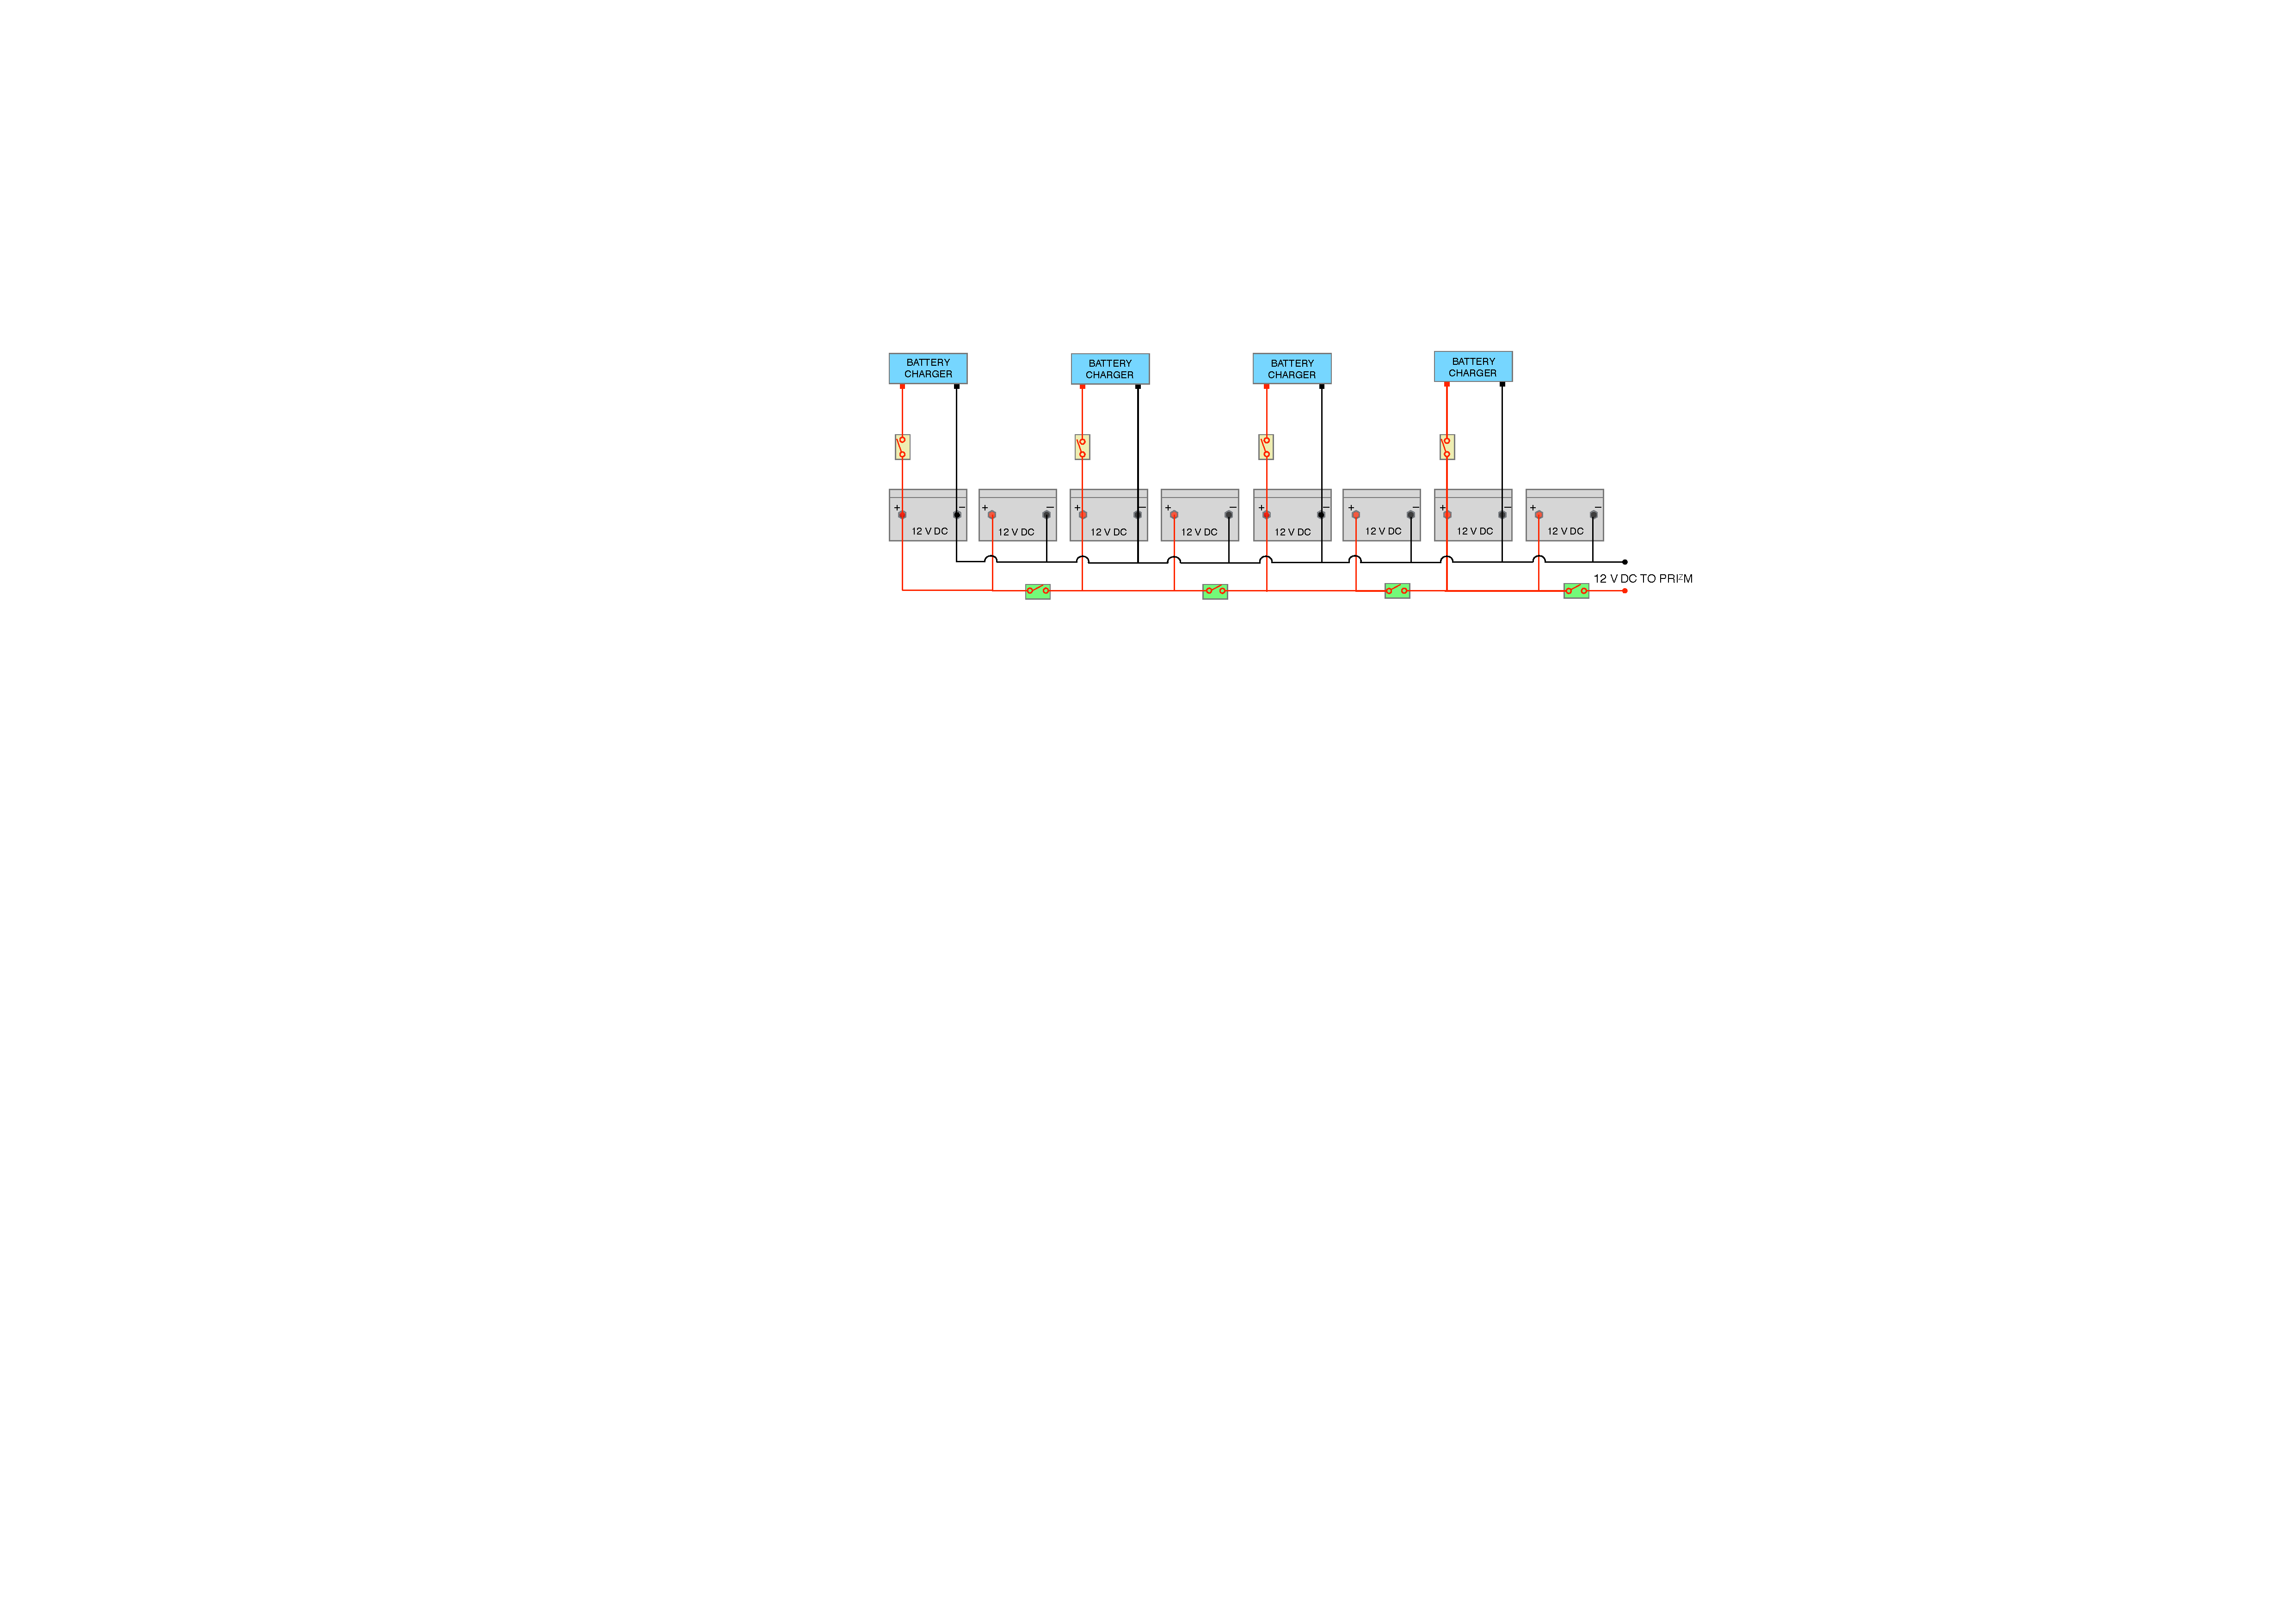
\includegraphics[width=\linewidth]{Figures/power_schematic}
	\caption{\prizm's power distribution chain consists of eight \SI{12}{\volt} \SI{200}{\ampere \hour} lead crystal batteries each. The batteries work in pairs that, through the green switches, are cascaded together. The battery pairs are disconnected during charging, and a single battery charger charges two batteries simultaneously. To connect the battery chargers, yellow switches are used. All yellow switches are turned OFF during the observation, and all green switches are powered ON.}
	\label{Fig:power}
\end{figure}

\section{Revised \prizm~Instrumentation}

This section describes revisions made to some of the \prizm\ subsystems in preparation for the 2020 voyage to improve functionality and performance. The first stage, electronics enclosure redesign, will be discussed in the next subsections and the revised SSE enclosure. Due to COVID-19 restrictions, the redesigned first stage electronics and SSE were not fully integrated and tested, and this section reports the work that was completed before lockdowns began. The 2020 Marion voyage was canceled because of COVID-19\footnote{\url{https://www.timeslive.co.za/news/south-africa/2020-04-06-sas-expedition-to-marion-island-downsized-over-coronavirus-fears/}}. 

\subsection{First Stage Electronics (FSE)}

A new FSE and enclosure were proposed for the 2020 deployment. Figure~\ref{Fig:FSE_rev} shows the block diagram of the proposed FSE architecture. Off-the-shelf enclosures were used instead of the previous enclosures' custom geometry, and these new boxes provide slightly more room to house the SPDT switches, which are new additions. To ensure that the enclosure would accommodate all the FSE, dummy placeholder components were crafted and placed in the enclosures. Figure~\ref{Fig:FSE_archi} shows a nominal component layout. The perforated gray sheet serves as a mechanical breadboard for easy addition of new parts without drilling the enclosures. Two enclosures are attached back to back to service the two polarizations. Most of the housekeeping electronics are on the side of Figure~\ref{Fig:FSE_archi}, which is intended to be accessed from the east-facing column door, giving the human slight shelter from the prevailing wind. The only housekeeping breakout on the second enclosure is half of the one-wire thermometry bus.

\begin{figure}
	\centering
	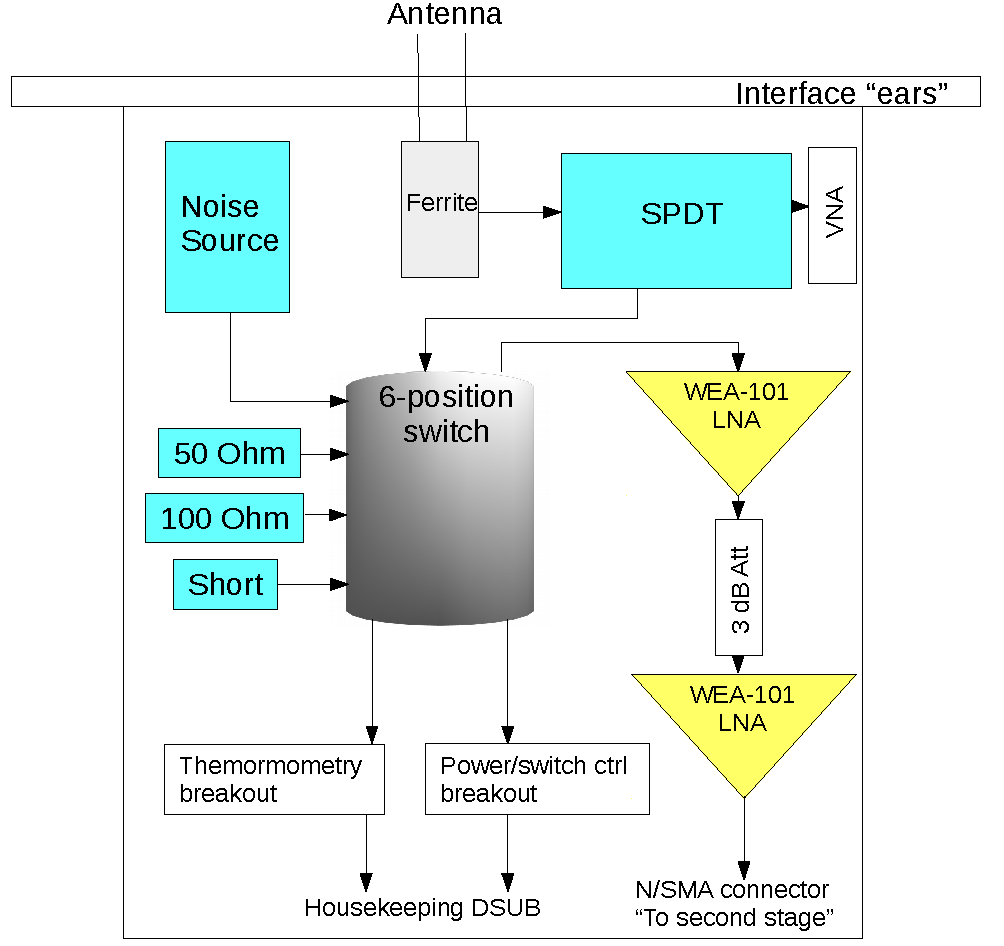
\includegraphics[width=0.7\linewidth]{Figures/FSE_rev}
	\caption{The block diagram of the proposed FSE achirtecture showing the 6-position switch connections, the breakouts for housekeeping, SPDT for controling the SP6T and amplification. The VNA is not permanently installed, and the box drawn indicates a connection point.}
	\label{Fig:FSE_rev}
\end{figure} 

The new box currently accommodates only one SPDT switch per side, and the plan is to add more switches to facilitate additional VNA measurements. The single SPDT switch does allow us to do VNA measurements of the antenna without disconnecting the antenna cables. The antenna cables connect the \prizm\ dipole to the calibrator switch. A right-angle adapter will be required on the SPDT to interface with the antenna cable. Without the SPDT switch in place, the S11 measurement looking into the antenna requires the antenna cable's physical disconnection from the 6-position switch. The new SPDT switch enables a selection of two positions, unlike the current \prizm\ configuration where the antenna signal is fed through the 6-position switch. The SPDT either selects the antenna signal to divert through the SPDT switch for VNA connection or continue as in the current configuration. In the new configuration, there is a free SMA port on the SPDT where the VNA can be connected or disconnected for measuring S11 looking into the antenna without connecting or disconnecting the cable. 

The terminal blocks for power and housekeeping signals have 16 positions total, so one is unused by the DB-15 breakout (and the SP6T switch can block the unused position). The filters in Figure~\ref{Fig:FSE_archi} are placeholders, but they are about the same size as the WEA-101 LNAs highlighted in yellow in Figure~\ref{Fig:FSE_rev}. In Figure~\ref{Fig:Terminal}, the incoming DB-15 connector is split out into two terminal blocks, and Table~\ref{Tab:Pinout} shows the connection configuration. The wall-mounted PCB has a 12V input and provides the LNAs with a 5V output and the one-wire thermometers with a 3.3V onboard output. All thermometers servicing both polarizations are ganged together on a single bus, so the headers are split accordingly across the enclosure's two halves.

\begin{figure}
	\centering
	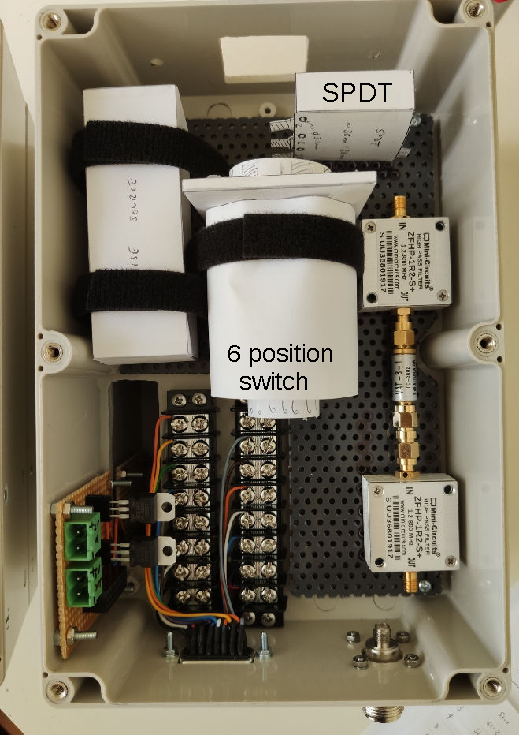
\includegraphics[width=0.5\linewidth]{Figures/FSE_archi}
	\caption{General layout of the components in the proposed FSE enclosure with dummy placeholders.}
	\label{Fig:FSE_archi}
\end{figure}

\begin{figure}
	\centering
	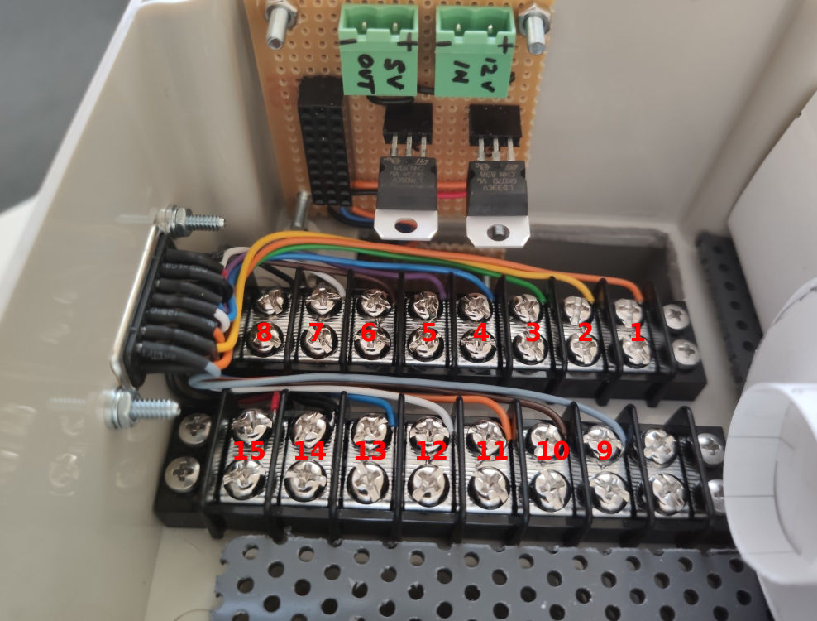
\includegraphics[width=0.7\linewidth]{Figures/Terminal}
	\caption{Housekeeping breakout. DB-15 pin assignments are annotated on the terminal blocks.}
	\label{Fig:Terminal}
\end{figure}

\begin{table}
	\centering
	\begin{tabular}{ c|c|c|c} 
		\hline
		DB-15 & Terminal Block & Colour & Function \\
		\hline
		\hline
		1 & L1 & Orange & S1-1 \\ 
		2 & L2 & Yellow & S1-2 \\ 
		3 & L3 & Green & S1-3 \\
		4 & L4 & Blue & S1-4 \\
		5 & L5 & Purple & S1-5 \\
		6 & L6 & Brown & S1-6 \\
		7 & L7 & White & S1-Reset \\
		8 & L8 & Black & Ground \\
		9 & R2 & Gray & S2-Ant \\
		10 & R3 & Brown & S2-Cal \\
		11 & R4 & Orange & Noise \\
		12 & R5 & White & Blank \\
		13 & R6 & Blue & Temp Sensor \\
		14 & R7 & Black & Ground \\
		15 & R8 & Red & 12 V \\
		\hline
	\end{tabular}
	\caption{Housekeeping pinout. Terminal block notation and numbering L and R denote left and right as viewed when the box is vertical, and numbers are from top to bottom. S1 denotes SP6T switch, S2 denotes SPDT switch.}
	\label{Tab:Pinout}
\end{table}


\subsection{Second Stage Electronics}

A revised Faraday cage for the SSE was designed using Autodesk Inventor Professional 2018, and the sheet metal box is shown in Figure~\ref{Fig:Enclosed}. The enclosure was revised so that each antenna has its SSE box.  There was no longer shared housekeeping RPi that binds the SNAP boards together. That was the main driver for separating the SNAP boards/ enclosures.

The switch circuit was redesigned as shown in Figure~\ref{Fig:newcontrol} by the schematic. Eight TLP3543 MOSFET output optocouplers were used to make the switch control circuit. Six of the optocouplers are used to control the 6-position switch, one is used for the reset, and the last one is used for the noise source. The circuit is designed to have a built-in precision real-time clock (RTC), and the chip used is the DS3231. Figure~\ref{Fig:control} shows the 3D view of the switch circuit PCB. The bigger green connector connects to the FSE via a DB15 connector mounted on the enclosure's front panel, and the smaller connector is for power distribution. Figure~\ref{Fig:Bottom} shows the female header, which is plugged directly into the RPi to form a stackable layout. The four mounting holes are precisely the same dimension as those of the RPi to fasten both of them simultaneously.

\begin{figure}
	\centering
	\includegraphics[width=\linewidth]{"Figures/new control"}
	\caption{Schematic diagram of the newly desined switch control circuit. In the new design, six out of eight MOSFET output optocouplers are used to control the 6-position switch, and the other two are used for reset and noise source. The circuit has a built-in RTC. RPi's GPIO pins are connected to the RTC and the optocouplers to controls the functionality.}
	\label{Fig:newcontrol}
\end{figure}


\begin{figure}
	\centering
	\begin{subfigure}[t]{0.52\textwidth}
		\centering
		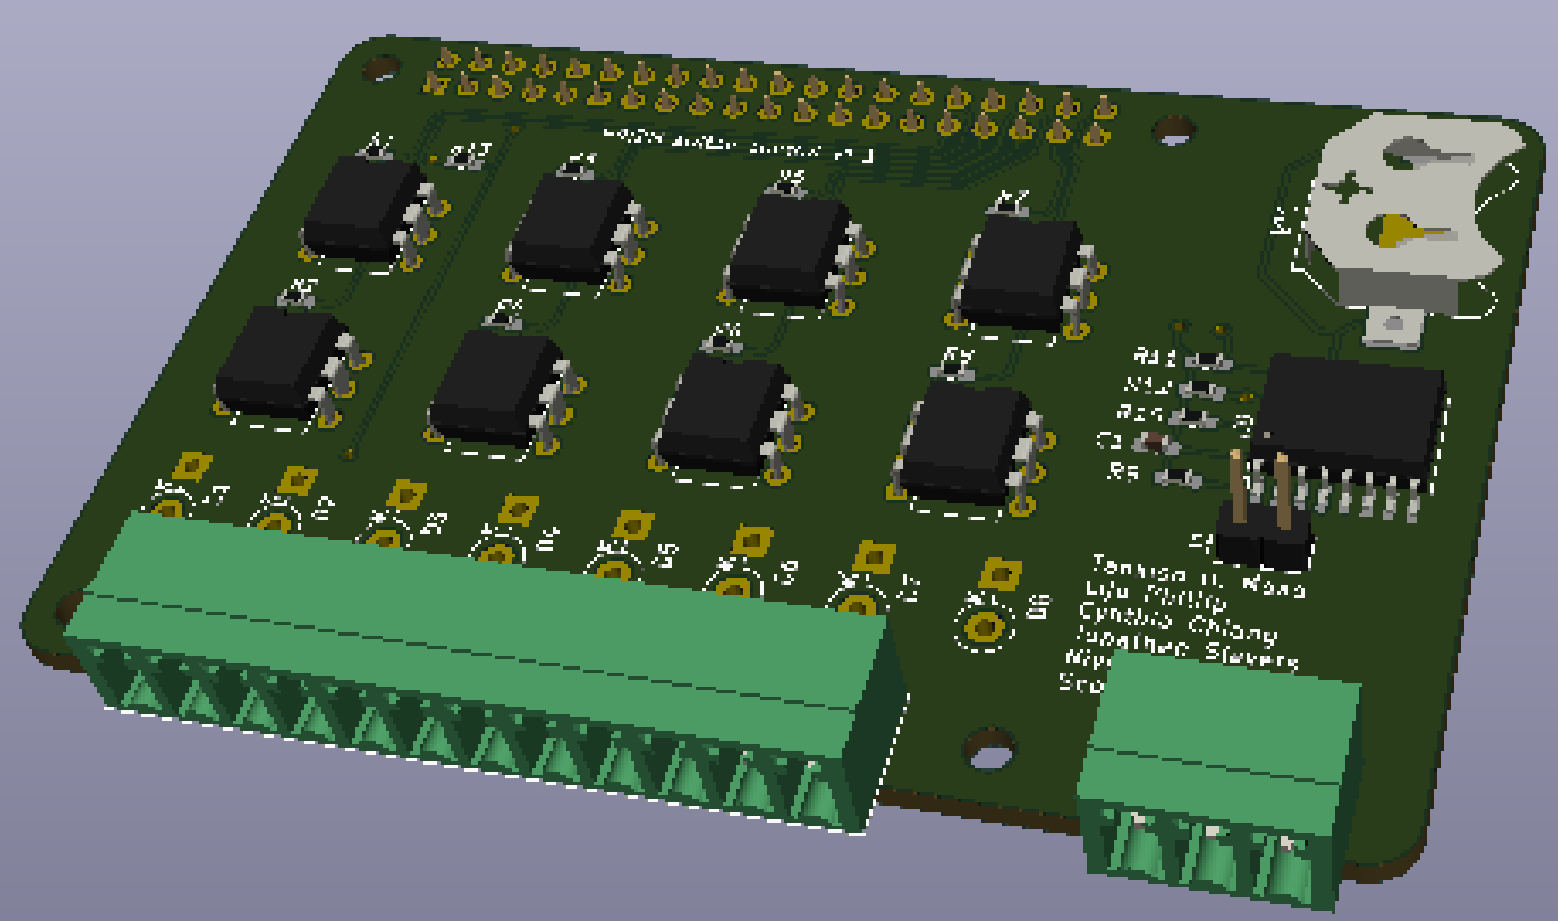
\includegraphics[width=\linewidth]{Figures/Top} 
		\caption{} \label{Fig:Top}
	\end{subfigure}
	\hfill
	\begin{subfigure}[t]{0.45\textwidth}
		\centering
		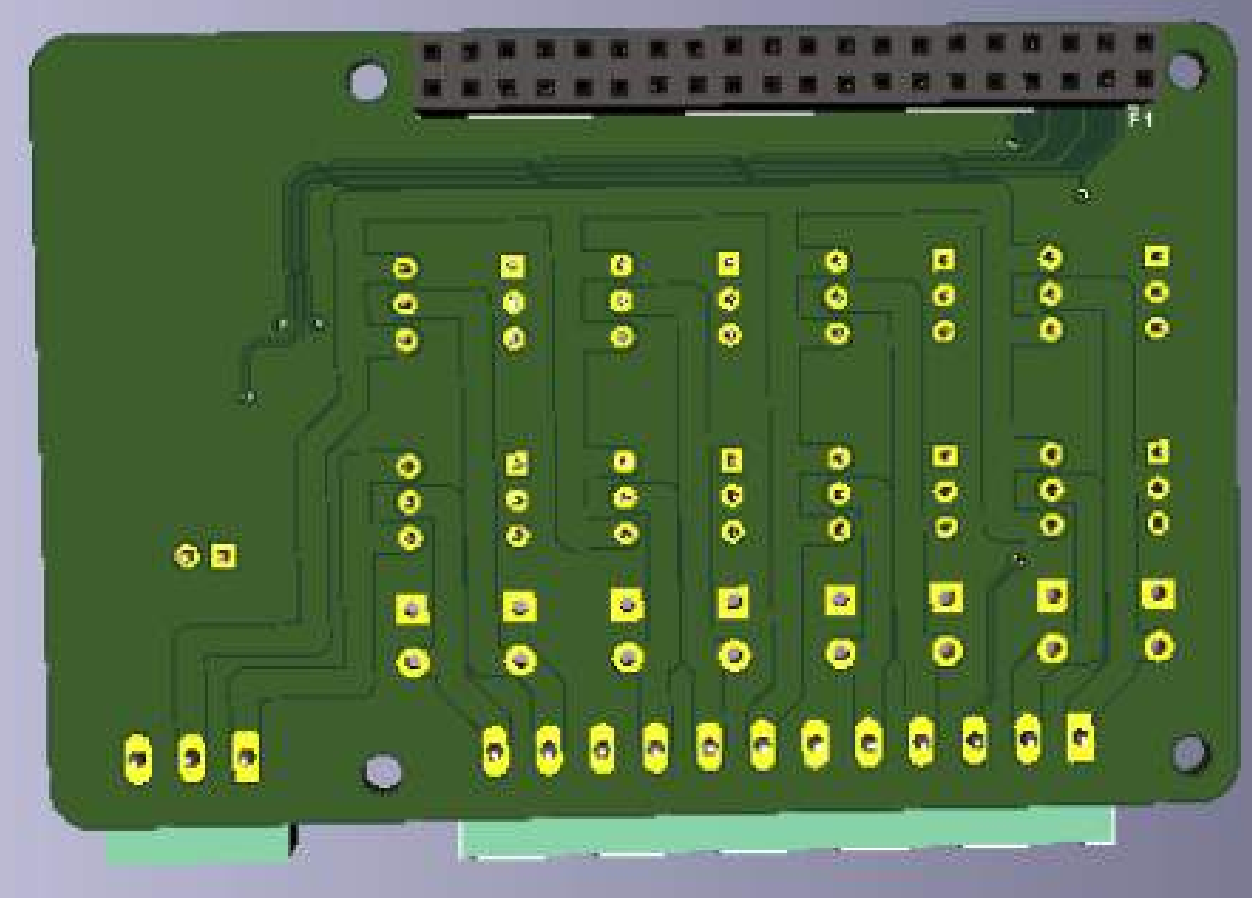
\includegraphics[width=\linewidth]{Figures/Bottom-compressed}
		\caption{} \label{Fig:Bottom}
	\end{subfigure}
	\caption{Top and bottom view of the newly designed switch control circuit. {\bf (a)} Top view. In the new design, six out of eight MOSFET output optocouplers are used to control the 6-position switch, and the other two are used for reset and noise source. {\bf (b)} Bottom view. The female header is connected to the GPIO pins of the RPi to form a stackable layout. The four mounting holes are exactly the same dimension as those of the RPi to fasten using taller fasteners.}
	\label{Fig:control}
\end{figure}

The main improvements to the new enclosure are listed below.

\begin{itemize}
	\item Increased and improved accessibility of all components. Because each enclosure now services only one antenna, all components can be accommodated on a single shelf that can be accessed from both sides.
	\item The design is folded laser cut sheet metal, unlike the separate brackets and flat sheets that make up the current design
	\item Easier and cheaper to assemble and manufacture
	\item User-friendly (the holes are already in place to tap and screw the components in place, and the lids are fastened using captive quarter-turn fasteners).
	\item It was designed to fit into a hiking backpack for easy carrying when hiking to the \prizm\ site. The current enclosure servicing both antennas is too large to carry on a hike to the site conveniently. The designed enclosure is \SI{\sim 400x280x110}{\milli \meter} and the current enclosure is \SI{\sim 300x470x240}{\milli \meter} 
	\item The new enclosure has a partitioned portion to accommodate the second stage RF electronics and ensure isolation from self-generated RFI from switching electronics elsewhere in the enclosure, as shown in Figure~\ref{Fig:Top Open}.
	\item A cooling fan was added to prevent thermal shutdowns of the SNAP board as shown in Figure~\ref{Fig:Bottom Open}.
	\item The switch control circuit was revised, and it is a stackable layout so that it sits on top of the RPi and connects directly to the GPIO pins.
	\item The RF absorbing material (3M Absorbing materials) is useful to line in the enclosure to avoid internal bounces from the RF noisy components, such as clocks of the digitizer and the switching from power supplies. That way, RFI is attenuated before reaching the amplifiers and other sensitive parts. 
\end{itemize}

A list of all components housed in the new enclosure is presented in Table~\ref{Tab:Components} with the quantities required. The front panel has feedthrough connectors that feed the signals/power in and out of the enclosure, as shown in Figure~\ref{Fig:Enclosed}. A non-isolated panel mount BNC connector is used to supply the main power to the box. Two N-F/SMA-F bulkheads (Amphenol 242163) are used for the second stage RF signals for both polarisations. Panel mount ethernet feedthrough (CONEC 17-101814) is for the data transfer between an enclosed RPi and the laptop. The filtered DB15 connector connects the FSE to the box.

\begin{table}
	\centering
	\begin{tabular}{ c|c}
		\hline
		Component & Quantity \\
		\hline
		\hline
		Meanwell 12VDC supply (RSD-60G-12) & 1 \\
		Terminal block for power breakout & 1 \\
		Buck converter & 2-4 \\
		Amplifier (ZX60-43-S+) & 2 \\
		High pass filter (HP-25+ HPF) & 2 \\
		Low pass filter (SLP-200+ LP) & 2 \\
		SNAP board	& 1 \\
		Switch control circuit & 1 \\
		Raspberry Pi 3, 3B+, or 4 & 1 \\
		Chronodot & 1 \\
		Adafruit GPS module & 1 \\		 
		\hline
	\end{tabular}
	\caption{A list of components that are housed inside the redesigned SSE enclosure.}
	\label{Tab:Components}
\end{table}

The enclosures were fabricated, and the sheet metal parts fitted together as designed, all the components were installed in the enclosures, and they fit the mounting holes that were already in place. COVID-19 lockdowns happened before dry-runs could be performed. 

\begin{figure}
	\centering
	\includegraphics[width=\linewidth]{"Figures/Top Open"} 
	\caption{CAD of an enclosure with the top lid open. The partioned portion is to avoid self-generated contamination from components with switching mechanisms. Some placeholders were mounted on the sheet metal design on Autodesk Inventor.} 
	\label{Fig:Top Open}
\end{figure}

\begin{figure}	
	\centering
	\includegraphics[width=\linewidth]{"Figures/Bottom Open"}
	\caption{The bottom view without the lid, showing the SNAP board and its cooling fan, and the RPi.} 
	\label{Fig:Bottom Open}
\end{figure}	

\begin{figure}
	\centering
	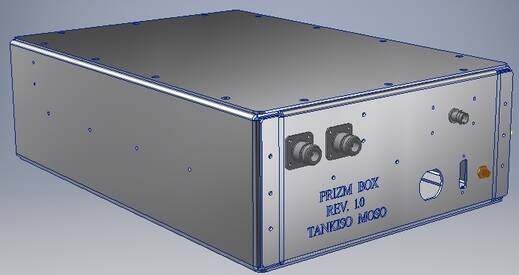
\includegraphics[width=\linewidth]{Figures/Enclosed}
	\caption{An enclosed box showing the connector placeholders and measured cutouts for other connectors that are not shown in this rendering}.	\label{Fig:Enclosed}
\end{figure}

	\chapter{Preliminary Data and Future Outlook}\label{s:Prel}

Figure~\ref{Fig:pathfinderresults} shows the results from the two-element interferometric array pathfinder discussed in \S\ref{s:pathfinder}. Figure~\ref{Fig:pathfinderresults} shows the auto- and cross- spectra where the waterfall plot was taken from one polarization over three days (June 18–21, 2018). The Galaxy rising/setting is visible in the structure. There are also ripples in frequency because of uncalibrated data, and the ripples arise from reflections in the cables. There is a qualitative difference between daytime and nighttime data, and this shows that the contamination from shortwave radio drops off significantly at night, when the ionosphere becomes quieter. It is distinctly visible from the figure that fringes show recurrent structure below $\sim$ \SI{10}{\mega\hertz} without data processing or data cuts. The auto spectra signal drop-off below $\lesssim$\SI{ 30}{\mega\hertz} results from the combined response of the antenna and the front-end electronics as shown in Figure~\ref{Fig:s11lwa}. These results demonstrate a proof of concept to proceed with the development of the autonomous stations.

\begin{figure}
	\centering
	\includegraphics[width=0.9\linewidth]{"Figures/pathfinder_results"}
	\caption{Spectra from a two-element ALBATROS pathfinder co-aligned polarization pair, shown as a frequency and time function. In the top and bottom rows, the auto- and cross-spectra are shown, respectively. The spectrum magnitudes are in uncalibrated ADC units on a logarithmic scale, and the amplitude of the cross-spectrum is around two orders of magnitude fainter than the auto spectra. The phase of the cross-spectrum can be seen in radians. The Galaxy's repeatable structure is evident in all plots over the 3-day time scale.}
	\label{Fig:pathfinderresults}
\end{figure}

\begin{figure}
	\centering
	\includegraphics[width=0.9\linewidth]{"Figures/s11 lwa"}
	\caption{Top: LWA antenna simulated S11, demonstrating the steep loss of signal below \SI{\sim 30}{\mega \hertz}. Bottom panel: for one of the polarization in the two-element ALBATROS pathfinder, the median uncalibrated auto spectrum compared to the crude sky signal estimate provided by the product (1-S11) with the product spectrum of nominal synchrotrons. Qualitatively, this simple model shows that the reduction in the antenna response is primarily responsible for auto spectrum power below \SI{\sim 30}{\mega \hertz}.}
	\label{Fig:s11lwa}
\end{figure}

An approximation of the instrumental consistency in gain can be obtained by comparing the total power between various days illustrated in Figure~\ref{Fig:pathfinderresults}. Within the frequencies of 30 and 40 MHz, it has been discovered that the RMS gain variations are below \SI{1}{\percent} and approximately \SI{0.04}{\percent} of the power at the standard noise on time scales of 3 seconds. The minimal noise indicates that relative calibration will yield sub-percent accuracy using auto spectra reported by each autonomous station. In the future, outright calibration will be extracted from the contrast of auto spectra with the co-located and thoroughly calibrated \prizm\ or Global Sky Model. Figure~\ref{Fig:pol1} shows the cross-spectra phases binned in nearby sidereal time as a subjective representation of the sky signal repeatability on tiny scales.

In this plot, about 372 hours of data are averaged, and no RFI extraction has been carried out. The high signal-to-noise fringe pattern, which is noticeable even marginally beneath $\sim$\SI{10}{\mega\hertz}, shows the verification of an idea for extending the ALBATROS array.

\begin{figure}
	\centering
	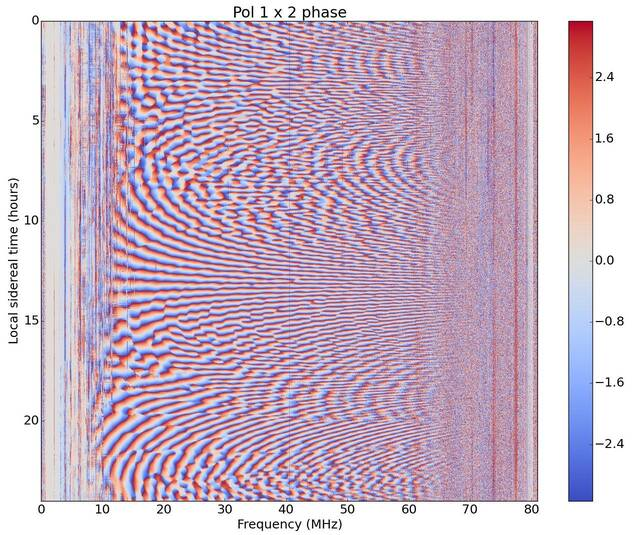
\includegraphics[width=0.7\linewidth]{Figures/pol1}
	\caption{Phases from the cross-correlation in the two-element ALBATROS pathfinder between two co-aligned polarizations. There are approximately 372 hours of data displayed here, binned in local sidereal time, and radians are the color stretch.}
	\label{Fig:pol1}
\end{figure}

Due to COVID-19 restriction and limited accessibility to the island, the data could not be retrieved from the single autonomous station pathfinder on Marion discussed in \S\ref{s:autonomous}; however, verification of the solar power system has effectively met the antenna station's power requirements. Because of the unavailability of data from Marion, baseband writing has been demonstrated by setting up a single-element pathfinder station at the McGill Arctic Research Station (MARS; \ang{79;26;}N, \ang{90;46;}W) Axel Heiberg Island, Nunavut, in July 2019. The RF signal chain shown in Figure~\ref{Fig:albatros1_schem} is similar to the MARS installation; although a solar power system was not used, instead manually charged batteries were used to supply power. The MARS RFI environment is much noisier than that of Marion Island. The ionospheric plasma cutoff frequency is higher than the average cutoff displayed in the Marion data because the data was taken during the peak of the Arctic summer. The MARS installation is appropriate for demonstrating baseband data writing, regardless of the distinct layout and RFI environment. 

Short chunks of baseband data that have been collected at different times over two adjoining frequency windows are displayed, \SIrange{5.3}{12.6}{\mega \hertz} and \SIrange{12.6}{20}{\mega \hertz}. In order to maintain auto spectrum data, the baseband data was registered with 4-bit quantization, which is not obtainable with 1-bit quantization. The one polarization auto spectra from the \albatros\ single-element pathfinder station that was set-up at MARS is shown in Figure~\ref{Fig:mars}, looking at the aggregated spectra that are directly registered by the SNAP board versus the spectra determined from baseband data. Altogether, the waterfall plots have the same 61-kHz frequency resolution, as defined by the spectrum resolution measured by the SNAP board. A logarithmic scale is shown in the waterfall plots to demonstrate the qualitative agreement for bright and faint spectral characteristics between the directly accumulated and baseband spectra. In order to demonstrate variations in the striking RFI characteristics that immerse the baseband data, the bottommost panels display the time-averaged spectra on a linear scale. Except where major immersion is present, the portion of baseband data with values at the 4-bit extrema is over-plotted with spectra. There is general consistency between the directly accumulated and baseband spectra. Figure~\ref{Fig:crossmars} shows waterfall phase plots calculated from the cross-correlation between two orthogonal polarizations of the ALBATROS pathfinder at MARS, looking at the directly accumulated and baseband data. Qualitatively, both sets of reported data concur, down to minor variations induced by the 4-bit quantization.

\begin{figure}
	\centering
	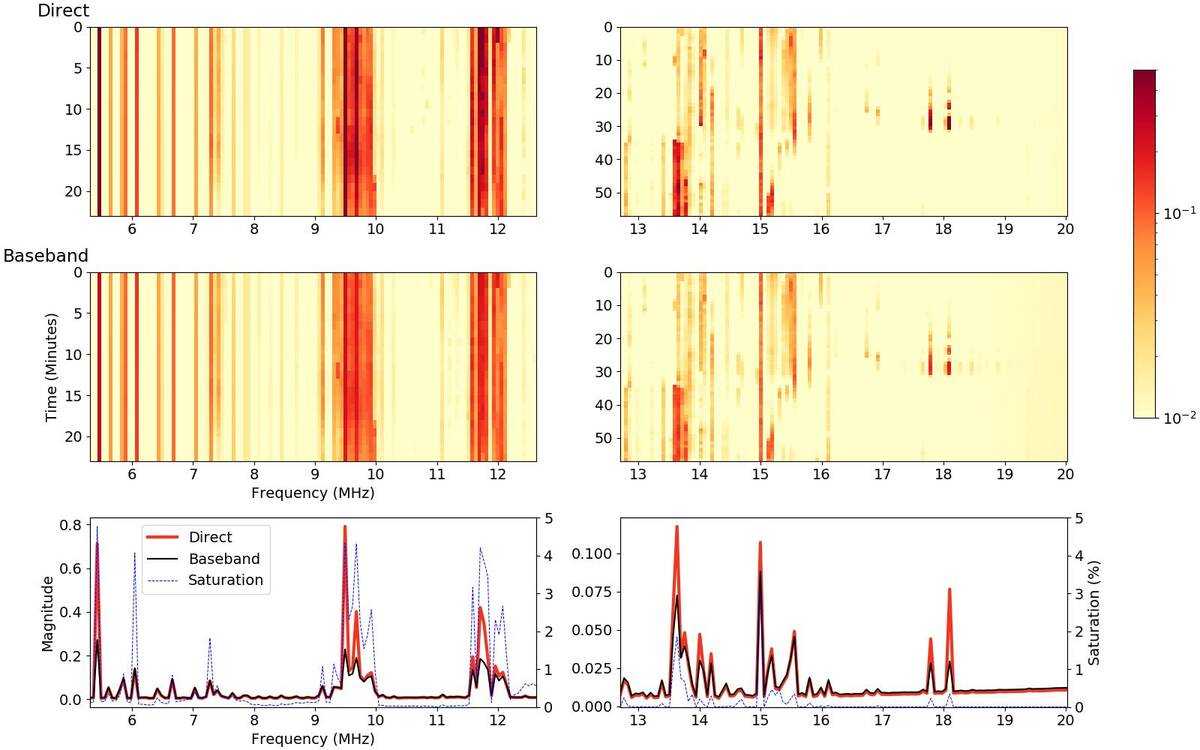
\includegraphics[width=\linewidth]{Figures/mars.jpg}
	\caption{Autospectra from the ALBATROS pathfinder at MARS for one polarization. The top row shows spectra directly accumulated by the SNAP board, and the middle row displays spectra with 4-bit quantization computed from baseband data. The two frequency windows are registered at two different periods, 5.3-12.6 MHz and 12.6-20.0 MHz, and both plots are displayed at a 61-kHz resolution.}
	\label{Fig:mars}
\end{figure}

\begin{figure}
	\centering
	\includegraphics[width=\linewidth]{"Figures/cross mars"}
	\caption{Cross-correlation phases between two orthogonal polarizations from the  ALBATROS pathfinder at MARS. The top row shows cross-spectrum phases that are directly accumulated by the SNAP board, and the bottom row shows phases with 4-bit quantization computed from baseband results. The two frequency windows, \SIrange{5.3}{12.6}{\mega \hertz} and \SIrange{12.6}{20}{\mega \hertz} are registered at two different times, and all 61-kHz resolution waterfall plots are shown.}
	\label{Fig:crossmars}
\end{figure}

\section{Conclusion and Future Outlook}

The design of \albatros\, a new interferometer that will image the radio sky at \SI{\sim 30}{\mega \hertz} using an array of autonomous antenna stations installed on Marion Island, has been presented. A clear demonstration of the repeatable sky signal visible from Marion down to $\lesssim$10~MHz without data processing or cutting, with a two-element, directly correlated pathfinder. The first autonomous prototype for \albatros\ powered solar panels have been constructed, and the electronics and database recording software have been successfully tested.

There are plans to improve the design of the future \albatros\ stations to be deployed in the coastal huts of Marion, with the evidence of the concept shown in the pathfinder instruments presented here. Currently, the LWA and FEE antennas are not designed for the lowest \albatros\ frequency observation, and potential antenna and FEE design modifications are being explored to enhance the low-frequency response of the calibration circuitry construction. Since future \albatros\ stations would be located farther away from the base and will be more challenging to access regularly, to store baseband data over extended periods, each station will require larger total disk space. A specially made low-power hard disk drive bank is being developed with $>$ 100~TB total capacity, and a USB multiplexer will be used to select and power only one hard drive at a time. The autonomous pathfinder of the station presented uses solar panels to charge the batteries and, as a future alternative for potential stations, the use of small wind turbines is explored. To compute time-domain data from the recorded channelized baseband, analysis tools are being built by inverting the polyphase filter bank while minimizing quantization and saturation artifacts.

A proposal for building a second \albatros\ array at MARS shown in Figure~\ref{Fig:MARS} in the high Arctic is being studied in addition to Marion Island. In July 2019, a single pathfinder antenna was mounted as defined in \S\ref{s:Prel} and observed for about three weeks to evaluate the RFI environment and ionospheric conditions. When fully operational, Marion and MARS \albatros\ will have new views across both hemispheres of the low-frequency sky.

\begin{figure}
	\centering
	\includegraphics[width=\linewidth]{Figures/MARS.pdf}
	\caption{The world map showing the location of MARS, where the \albatros\ will be viewing the Northern hemisphere sky.}
	\label{Fig:MARS}
\end{figure}

The \prizm\ experiment, which was the first radio astronomy project in Marion Island, was discussed, and the revision of the subsystems was presented. The new FSE was designed, and further modifications are still going to be employed. The SSE enclosure was successfully designed, fabricated and the enclosure parts were fitted together. The new switch control circuit design was successful, and it fitted the stacked layout on top of the RPi. All the \prizm\ modifications are still going to be employed on the next Marion voyage, hopefully in April 2021. 

	
	\bibliographystyle{unsrtnat}   
	\bibliography{TH_Moso_MSc_Thesis}{}
	
\end{document}
